\documentclass[12pt]{article}
\usepackage[utf8]{inputenc}
\usepackage{amsmath, amssymb}
\usepackage[margin=1in]{geometry}
\usepackage{enumitem}
\usepackage{parskip} 
\usepackage[allcolors=blue]{hyperref}
\usepackage{graphicx}
\usepackage{titlesec}
\usepackage{fancyhdr}
\usepackage{wasysym}
\usepackage{amsthm}
\usepackage{xcolor}
\usepackage{minitoc}
\usepackage{appendix}
\usepackage{tikz-cd} 
\usepackage{upgreek}
\usepackage{caption}
\captionsetup[figure]{font=small}
\hypersetup{colorlinks=true, urlcolor=blue}

\setenumerate[0]{label=(\alph*)}

\numberwithin{equation}{subsection}
\numberwithin{figure}{subsection}
%\renewcommand{\thefigure}{\arabic{section}.\arabic{subsection}.\arabic{figure}}
\swapnumbers
\newtheorem{thm}[subsection]{Theorem}
\newtheorem{lem}[subsection]{Lemma}
\newtheorem{defn}[subsection]{Definition}
\newtheorem{prop}[subsection]{Proposition}
\newtheorem{corr}[subsection]{Corollary}
\newtheorem{fact}[subsection]{Fact}

\newtheoremstyle{note}% <name>
{3pt}% <Space above>
{3pt}% <Space below>
{}% <Body font>
{}% <Indent amount>
{\itshape}% <Theorem head font>
{.}% <Punctuation after theorem head>
{.5em}% <Space after theorem headi>
{}% <Theorem head spec (can be left empty, meaning `normal')>
\theoremstyle{note}
\newtheorem{example}[subsection]{Example}
\newtheorem{remark}[subsection]{Remark}
\newtheorem{warning}[subsection]{Warning}
\newtheorem{terminology}[subsection]{Terminology}
\newtheorem{notation}[subsection]{Notation}

\titleformat{\subsection}
  {\normalfont\fontsize{12}{12}\bfseries}{\thesubsection}{1em}{}
 
 \titleformat{\section}
  {\normalfont\fontsize{14}{14}\bfseries}{\thesection}{1em}{}
 
\pagestyle{fancy} 

%\rhead{Section \thesection}

\setcounter{tocdepth}{1}
\renewcommand{\contentsname}{Sections}

\renewcommand*{\thefootnote}{[\arabic{footnote}]}
\newcommand{\curl}{\mathrm{curl\,}}
\newcommand{\R}{\mathbf{R}}
\newcommand{\C}{\mathbf{C}}
\newcommand{\Z}{\mathbf{Z}}
\newcommand{\N}{\mathbf{N}}
\newcommand{\Pol}{\mathbf{P}}
\newcommand{\img}{\mathrm{img\,}}
\newcommand{\dv}{\mathrm{div\,}}
\newcommand\tr[1]{\mathrm{tr}(#1)}
\newcommand\GL[1]{\mathrm{GL}(#1)}
\newcommand\On[1]{\mathrm{O}(#1)}
\newcommand\SO[1]{\mathrm{SO}(#1)}
\newcommand\SL[1]{\mathrm{SL}(#1)}
\newcommand\Span[1]{\mathrm{Span}\left\{#1\right\}}
\newcommand\nul[1]{\mathrm{null}(#1)}
\newcommand\adj[1]{\mathrm{adj}(#1)}
\newcommand\col[1]{\mathrm{col}(#1)}
\newcommand\row[1]{\mathrm{row}(#1)}
\newcommand\rank[1]{\mathrm{rank}(#1)}
\newcommand\Mat{\mathrm{Mat}}
\newcommand\ip[2]{\langle #1, #2\rangle}
\newcommand\m[1]{\begin{pmatrix}#1\end{pmatrix}} 
\newcommand\proj[2]{\mathrm{proj}_{#1}(#2)}

\makeatletter
\let\c@equation\c@figure
\makeatother

\makeatletter
\renewcommand*\l@section{\@dottedtocline{1}{1.5em}{2.3em}}
\makeatother

\setcounter{section}{-1}
\setlength{\headheight}{15pt}
 \addtolength{\topmargin}{-3pt}
 
\newenvironment{amatrix}[1]{%
  \left(\begin{array}{@{}*{#1}{c}|c@{}}
}{%
  \end{array}\right)
}

\begin{document}

\title{ \textbf{Linear Algebra \\ Course notes and exercises}}
\author{\small Prepared by: Duncan Clark, PhD}
\date{\small 
%Spring semester 24--25 AY \\ 
\textit{Last updated}: \today}
\maketitle 


\tableofcontents 


\newpage

\section{Preface}


\subsection{How to use these notes} These course notes and exercises are intended to serve as an aid to the class. Notes for sections contain big picture ideas, definitions, statements of theorems, and worked out examples (when appropriate). They are not meant as a substitution for attending class, but rather as a reference. I \textit{highly encourage} you to work through the exercises and not just look up answers. My intention is to have problems at various difficulty levels (problems marked with an asterisk * are intended to be challenge problems). Keep in mind, the struggle you experience when trying and failing at a problem \textit{is} learning---keep at it and ask me questions as you have them. 

Terms in \textbf{bold} are typically (parts of) definitions. Definitions are the basis of mathematics, and this course is one in your mathematical journey where they become very important. In this course we also learn a handful of nontrivial theorems. In addition to solving problems, a good place to start with studying is to know the definitions and theorems for the content covered: i.e., know why the definition does what we want it to, and  what each of the theorems are, how to use them, and why the conditions are needed.






\subsection{Helpful computational tools}
\begin{itemize}
	\item \textbf{Online calculator} for quickly checking calculations (such as determinant, inverse, diagonalization, etc.) \href{https://www.wolframalpha.com/}{WolframAlpha}
	\item \textbf{Additional software}.
	\begin{itemize}
	\item \href{https://numpy.org/}{Numpy} is a computational package for Python that includes most of the standard linear algebra algorithms.
	\item  \href{https://www.wolfram.com/mathematica/}{Wolfram Mathematica} is an extremely powerful language, but with a much higher learning curve. You can get a license through the tech support office
	\item \href{https://www.mathworks.com/products/matlab.html}{MATLAB} can also make really nice pictures for you, but has a similar barrier to entry as Mathematica
	\end{itemize}
\end{itemize}



\subsection{Licensing}
This note and exercise packet is licensed under the \href{https://creativecommons.org/licenses/by-nc-sa/4.0/}{Creative Commons CS BY-NC-SA 4.0 License}. \[
\includegraphics{Images/by-nc-sa}\]
\newpage


\section{Systems of linear equations}
The subject of linear algebra is concerned with \textbf{linear equations} and systems thereof. 

\begin{defn}
	A \textbf{linear equation} in the variables $x_1,x_2,\dots, x_n$ is any equation of the form \begin{equation} a_1 x_1 + a_2 x_2+ \cdots + a_nx_n =b\end{equation}
	for constants $a_1,a_2,\dots,a_n$ and $b$.
\end{defn}

This definition is somewhat incomplete though: what does it mean \textit{constant}? what sort of terms are the variables $x_1,x_2,\cdots,x_n$ allowed to be? For the purpose of our class, we will primarily concern ourselves with linear equations \textit{of real numbers}---that is, where the constant terms and variables $x_i$ are all real numbers. However, linear algebra as a subject allows for much greater abstraction than this\footnote{We may consider equations with complex number coefficients later on this term. Generally, coefficients to a linear system can come from any \textit{ring}.}. 

\subsection{Systems of equations} 
A \textbf{system} of linear equations is  a (finite) collection of linear equations. Sometimes we'll write ``linear system" as shorthand for ``linear system of equations". It's also sometimes useful to have a name to refer to a system by, typically we'll use a script letter ``s": $\mathcal{S}$. 

\begin{terminology} Let's say we're given a system of linear equations in the given variables of $x_1,x_2,\cdots,x_n$. A \textbf{solution} to this system is an $n$-tuple $s=(s_1,s_2,\cdots,s_n)$ such that substituting $x_1=s_1, x_2=s_2, \cdots, x_n=s_n$ yields true statements for each equation in the system. 
 
The \textbf{solution set} of a given system of linear equations is the collection of all solutions. If a given system has any solutions at all it is called \textbf{consistent}. Of note is that not all systems of equations are consistent, if a given system has no solutions it is called \textbf{inconsistent}. Two systems which have the same solution set are called \textbf{equivalent}.
\end{terminology}

\begin{example}[``Substitution method"]
For instance, the following is a system of linear equations in the variables $x,y$ and $z$: 
\begin{align}
	2x - 3y+z &= 9 \nonumber \\
	x+y&=2 \nonumber \\
	2x+3z &=6 \label{ex-sub}
\end{align}
How would find a solution to this system? Most familiar is probably the method of substituting: in this case, rearranging the second and third equations and $y=2-x, z=(6-2x)/3$, substituting these in for $y$ and $z$ in the first, and solving for $x$. This yields the sole solution to this system, \[(x,y,z)=(3,-1,0)\]

This method is fine for small systems (typically $n\leq 3$ or $4$), but becomes increasingly tedious as the number of variables and equations gets large. What's more, is that not all systems of equations have a just a single solution (or any solution at all). The method of substitution misses a lot of subtlety in the \textit{structure} of solution sets for systems of linear equations. 
\end{example}

\subsection{Geometric interpretation of systems of equations}
It's useful to have a geometric understanding of what's happening when we solve such linear systems. Let's start by recalling the following facts:
\begin{fact}$~$
	\begin{itemize}
		\item A linear equation in two variables defines a line in the plane
		\item A linear equation in three variables defines a plane in 3D space
	\end{itemize}
\end{fact}
This is true more generally as well: \textit{A linear equation in $n$ variables defines an $(n-1)$-dimensional ``flat region"\footnote{Often (somewhat uncreatively) called a \textit{hyperplane}} of $n$-dimensional space}. This obviously becomes harder to visualize, but the intuition from 2- and 3-dimensional space is often enough to get the picture. A solution to a system of linear equations is then a point $s$ which simultaneously lies on all lines/planes/hyperplanes (etc.) of a given system of equations. 

\begin{remark}As we'll see soon, \textit{linear} systems of equations have solutions sets which are highly structured. This is certainly not the case for \textit{non-linear} systems of equations (which are in general significantly harder to solve). The upshot is that within the field of linear algebra we are able to \textit{completely} describe the solution sets of linear systems, it just takes a bit of work. \end{remark}


\subsection{Exercises}
\begin{enumerate}[label=\arabic*.]
\item Determine the solution sets to the following linear systems, use either substitution or elementary row operations applied to the augmented matrix of the system.
\begin{enumerate}
	\item \; $\begin{aligned}[t] 2s+t&=1 \\ s-2t &=2 \end{aligned}$
	
	\item \;
	$\begin{aligned}[t] 
	 x+4z&=-4 \\ x+3y+3z&=-2 \\ 3x+7y+5z&=6
	\end{aligned}$
	\item \; $\begin{aligned}[t]
		x-3y&=5\\ y+5z-x&=2\\y+z&=0
	\end{aligned}$
	\item\; $\begin{aligned}[t] u-6v+4w&=-1 \\ 2v-7w&=4 \\ w+2y&=-3 \\ 3w+y&=6\end{aligned}$
\end{enumerate}

\item Determine all possible ways that three planes in 3D space can intersect.

\item True or False. Determine if the following statements are true or false. Justify your answer
\begin{enumerate}
	\item A linear system can have \textit{exactly} two solutions
	\item Any linear system with three equations in two variables is inconsistent.
	\item The following linear systems are equivalent \[ \begin{aligned} x-2y+z&=0  \\ 5y-2z &= 8 \\ 4x-y+3z&=-6 \end{aligned} 
	\qquad\qquad \qquad  \begin{aligned} 3y-z&=8 \\ 
	 2y-z&=14 \\
	 7y-z&=-6\end{aligned} \]
	\item There are no values of $d$ such that the following system is consistent: \begin{align*} x+3y &=1 \\2x+6y&=d\end{align*}
	\end{enumerate}
\end{enumerate}
Additional suggested exercises: \textit{Lay} section 1.1

\section{Row operations and echelon form}


While it's always technically possible to enumerate the solutions of a system of linear equations using substitution, once the number of variables gets ``large" (typically $\geq 5$), working with the equations hands-on becomes somewhat unruly. 

\subsection{Enter the matrix}
{Matrices}\footnote{\textit{Matrix} is the singular, you can write the plural form of this word either as \textit{matrices} or \textit{matrixes}. The etymology of the word matrix in this use is a bit peculiar, the English word \textit{matrix} comes from the Latin \textit{mater}---meaning ``mother".} are an algebraic tool used to abstractify (among other things) the work done in the substitution method for solving linear systems. For us, matrix algebra is the main computational tool we'll be developing this term. It is similar to the algebra of real numbers that you are used to, but with some crucial differences. Since matrices play such a fundamental role in mathematics (and engineering and science), it's worthwhile to spend some time discussing what specifically they are. 

\begin{defn}
Let $n,m$ be integers $n,m \geq 1$. An \textbf{$m\times n$ matrix} is a rectangular grid of entries: \begin{equation} A=\begin{pmatrix} a_{1,1} & a_{1,2} & \cdots & a_{1,n} \\
a_{2,1} & a_{2,2} & \cdots & a_{2,n} \\
\vdots & \vdots & & \vdots \\
a_{m,1} & a_{m,2} &\cdots & a_{m,n}
\end{pmatrix} \end{equation}
\end{defn}
The terms $a_{i,j}$ for $1\leq i\leq m$ and $1\leq j\leq n$ are called the \textit{coefficients} of the matrix $A$. For now we'll just be considering matrices whose entries are real numbers. An $m\times n$ matrix always has $m$ rows and $n$ columns (i.e., the number of rows is read first). If $m=n$, $A$ is called a \textbf{square} matrix. 

Generic names for the coefficients of a matrix can be defined by writing $A=\{a_{i,j}\}$, or just writing $A_{i,j}$ to denote the $i,j$ entry of $A$. When necessary, you can add subscripts to denote what the range of $i$ and $j$ should be: for instance if $A$ is an $m\times n$ matrix you'll sometimes see the (very cluttered) notation \[ A=\{a_{i,j}\}_{1\leq i\leq m, \; 1 \leq j \leq n}\]

\subsection{Matrices from linear systems}

Any linear system of equations has associated to it two matrices: the \textbf{coefficient matrix} and \textbf{augmented matrix}. The key is that determining the solution set of a system of linear equations can be achieved by ``elementary row operations" applied to the system's associated augmented matrix. 

\begin{defn} 
Given a system of equations $\mathcal{S}$  \begin{align} 
a_{1,1}x_1+a_{1,2}x_2+\cdots + a_{1,n}x_n&=b_1 \nonumber \\
a_{2,1}x_1+a_{2,2}x_2+\cdots + a_{2,n}x_n&=b_2 \nonumber \\ 
 &\vdots \nonumber  \\
a_{m,1}x_1+a_{m,2}x_2+\cdots + a_{m,n}x_n&=b_m \end{align}
the \textbf{coefficient matrix} is the matrix \begin{equation} C_{\mathcal{S}}=\begin{pmatrix} a_{1,1} & a_{1,2} & \cdots & a_{1,n} \\
a_{2,1} & a_{2,2} & \cdots & a_{2,n} \\
\vdots & \vdots & & \vdots \\
a_{m,1} & a_{m,2} &\cdots & a_{m,n}
\end{pmatrix} \end{equation}
and the \textbf{augmented matrix} is the matrix \begin{equation} A_{\mathcal{S}}=\begin{pmatrix} a_{1,1} & a_{1,2} & \cdots & a_{1,n} & b_1 \\
a_{2,1} & a_{2,2} & \cdots & a_{2,n} & b_2\\
\vdots & \vdots & & \vdots & \vdots \\
a_{m,1} & a_{m,2} &\cdots & a_{m,n} & b_m
\end{pmatrix}\end{equation}
\end{defn}

\begin{remark}Note that the augmented matrix contains the coefficient matrix if you ignore the right-most column. It's often customary to typeset the augmented matrix of a linear system in a way that ``sets aside" the right-most column (for reasons we'll soon see why) as follows:
\begin{equation}\begin{amatrix}{4} a_{1,1} & a_{1,2} & \cdots & a_{1,n} & b_1 \\
a_{2,1} & a_{2,2} & \cdots & a_{2,n} & b_2\\
\vdots & \vdots & & \vdots & \vdots \\
a_{m,1} & a_{m,2} &\cdots & a_{m,n} & b_m
\end{amatrix}\end{equation}
If you see this notation, you can mentally ``ignore" the vertical bar, this is just an $(m+1)\times n$ matrix after all. 
\end{remark}


\begin{example} Returning to the system from \eqref{ex-sub} we have the following coefficient matrix
\[ \begin{pmatrix} 2 & -3 & 1 \\ 1 & 1 & 0 \\ 2 & 0 & 3\end{pmatrix} \]
and augmented matrix \[ \begin{amatrix}{3}  2 & -3 & 1 & 9 \\ 1 & 1 & 0 & 2 \\ 2 & 0 & 3 & 6 \end{amatrix}\]
\end{example}

\begin{remark}It's worth pointing out that any matrix can be viewed as the coefficient matrix of a given linear system. This linear system is not unique, as the constants on the right hand side of the equations would not be specified. Moreover, any matrix with at least two columns can be viewed as the \textit{augmented} matrix to a given linear system, which is unique. 
\end{remark}

\subsection{Row operations}
On its own, just writing down the coefficient or augmented matrix to a linear system is not much of a help. However, what we'll learn now is a process for finding the solution set to a linear system by algebraically manipulating the coefficient/augmented matrix of that system. 

Such algebraic manipulations are called  \textbf{elementary row operations}\footnote{There's going to be a long standing tradition in linear algebra to overload terms of things with a ton of adjectives, if you just call these ``row operations" that's also fine, the word ``elementary" isn't pulling any real weight here.}. The idea is that we can take a given system $\mathcal{S}$ and replace it by an equivalent system which has the same solution set, with the intention that this system be easier to determine the solution set of. 

\begin{defn}[Elementary row operations] Given a matrix $A$, any of the following manipulations is called an \textbf{elementary row operation} (to $A$). 

\begin{itemize}
	\item Add a row to another row
	\item Swap the positions of any two rows
	\item Multiply the entries of a row by a given (nonzero) constant
\end{itemize}
\end{defn}

Some useful notation: if we apply an elementary row operation to matrix $A$ to achieve matrix $B$, let's write $A\sim B$. 
\begin{fact}
	Given a linear system $\mathcal{S}$, any elementary row operation done to the augmented matrix of $\mathcal{S}$ yields an equivalent linear system.
\end{fact}
Said differently, elementary row operations do not change the solution set of (the linear system associated to) an augmented matrix\footnote{It's worth pointing out the algorithmic efficiency of row reduction is $O(n^3)$ (meaning, that the number of steps required to reduce an $n\times n$ matrix is going to grow like a constant multiple of $n^3$). In particular, this is a problem that can be solved in polynomial time: your computer is very efficient at row reducing very large matrices, which is good because typical applications of linear algebra (e.g., machine learning) involve matrices of thousands (or more) rows or columns}. Or even more differently, for augmented matrices $A,B$ if $A\sim B$ then then systems associated to $A$ and $B$ are equivalent. 



\begin{example} \label{ex-row-ops}  In full gory detail, outlined below is (a sequence of) elementary row operations applied to the augmented matrix from \eqref{ex-sub} to produce an equivalent system with an ``easier to parse" solution. On the right is a description of the row operation applied at each step (writing ($n$) for the $n$-th row)
{ \allowdisplaybreaks\begin{align*} \begin{amatrix}{3}  2 & -3 & 1 & 9 \\ 1 & 1 & 0 & 2 \\ 2 & 0 & 3 & 6 \end{amatrix} \sim & 
\begin{amatrix}{3}  1 & 1 & 0 & 2 \\ 2 & -3 & 1 & 9 \\  2 & 0 & 3 & 6 \end{amatrix} & \text{swap (1) and (2)}\\
\sim & \begin{amatrix}{3}  1 & 1 & 0 & 2 \\ 0 & -5 & 1 & 5 \\  0 & -2 & 3 & 2 \end{amatrix}& \text{subtract $2\cdot $(1) from (2) and from (3)} \\
\sim & \begin{amatrix}{3}  1 & 1 & 0 & 2 \\ 0 & -10 & 2 & 10 \\  0 & -10 & 15 & 10 \end{amatrix} & \text{multiply (2) by 2 and (3) by 5}\\
\sim & \begin{amatrix}{3}  1 & 1 & 0 & 2 \\ 0 & -10 & 2 & 10 \\  0 & 0 & 13 & 0 \end{amatrix} &\text{subtract (2) from (3)}\\
\sim & \begin{amatrix}{3}  1 & 1 & 0 & 2 \\ 0 & -10 & 2 & 10 \\  0 & 0 & 1 & 0 \end{amatrix} &\text{multiply (3) by 1/13} \\
\sim & \begin{amatrix}{3}  1 & 1 & 0 & 2 \\ 0 & -5 & 1 & 5 \\  0 & 0 & 1 & 0 \end{amatrix} & \text{multiply (2) by 1/2}\\
\sim & \begin{amatrix}{3}  1 & 1 & 0 & 2 \\ 0 & -5 & 0 & 5 \\  0 & 0 & 1 & 0 \end{amatrix} & \text{subtract (3) from (2)} \\
\sim & \begin{amatrix}{3}  1 & 1 & 0 & 2 \\ 0 & 1 & 0 & -1 \\  0 & 0 & 1 & 0 \end{amatrix} & \text{multiply (2) by -1/5}\\
\sim & \begin{amatrix}{3}  1 & 0 & 0 & 3 \\ 0 & 1 & 0 & -1 \\  0 & 0 & 1 & 0 \end{amatrix}& \text{subtract (2) from (1)}\\
\end{align*}}
Thus we've turned the original system \eqref{ex-sub} into the system $\mathcal{S}$' given by  \begin{align} x &= 3 \nonumber \\ y&=-1 \nonumber\\ z&=0 \end{align} From here it's pretty simple to read off the solution, the given triplet $(x,y,z)=(3,-1,0)$. Moreover, any other solution to $\mathcal{S}$ would \textit{have to} be a solution to $\mathcal{S}$', and since it's ``clear'' that $\mathcal{S}'$ only has the one solution, we've now found the entire solution set to $\mathcal{S}$. 
\end{example}

\subsection{Echelon form}
The goal of elementary row operations being to ``simplify" the reading-off of the solution set of a linear system, it's perhaps unclear what the desired ``simplified" form of a given matrix should be. One answer is called \textit{echelon %\footnote{The word \textit{echelon} meaning ``rank" or file}
 form} as described below (informally, a matrix in echelon form has a bunch of 0s in the lower left hand corner that make the shape of a pixelated triangle).
\begin{defn}
	A matrix is said to be in \textbf{echelon form} if the following are satisfied
	\begin{itemize}
		\item All nonzero rows are above any rows of zeros
		\item Each leading entry (i.e., first non zero entry) of a row is farther to the right than the leading entry of the row above it
		\item In a given column, all entries below a leading entry are zero
	\end{itemize}
	A matrix is said to be in \textbf{reduced echelon form} if it is in echelon form and further satisfies:
	\begin{itemize}
		\item Each leading entry is a 1
		\item Each leading 1 is the only nonzero entry in its column
	\end{itemize}
\end{defn}
Reduced echelon form is the easiest to read the solution set off of, as we've seen in example \ref{ex-row-ops} and will see more throughout this term. I leave it to you to convince yourself of the following fact:
\begin{fact} Given a matrix $A$, there is a unique matrix $B$ in reduced echelon form such that $B$ is obtained from $A$ by elementary row operations. 
\end{fact}
While it's good to get practice doing row operations by hand, it ultimately becomes (extremely) tedious to do by hand. Fortunately, we have very efficient algorithms and very fast computers which are more than happy to do these calculations for us\footnote{It's not unreasonable to call your graphics card a big linear algebra calculator, or at least certain cores of it.}.

\subsection{Free variables}
Suppose you are given a linear system of equations, and as a result of row operations have the following matrix in reduced echelon form: \begin{equation} \begin{amatrix}{3} 1 & 0 & 3 & 1 \\ 0 & 1 & -1 & -3 \end{amatrix}\end{equation}
How would you describe the solution set? 
In equations, this would look like: \begin{equation} \label{ex-free-var} x_1 + 3x_3 = 1, \quad x_2-x_3=-3 \end{equation} The thing is, there is more than one possible solution here: In this case, we can describe variables $x_1$ and $x_2$ \textit{in terms} of the third variable $x_3$. In such a situation we call $x_3$ a \textbf{free variable} (also called \textbf{independent variable})---idea being that $x_3$ is not constricted, any real number can be plugged in for $x_3$ so long as the other variables are calculated by the equations from \eqref{ex-free-var}. The solution for this system is then described as follows:  \begin{align} x_1&=1-3x_3 \nonumber \\ x_2&=x_3-3 \nonumber  \\ x_3 &\text{ is free} \label{ex-free-var-sol} \end{align}
The variables $x_1,x_2$ are not free (often called \textbf{bound} or \textbf{dependent}). So, one such solution would come from $x_3=0$, i.e., $(x_1,x_2,x_3)=(1,-3,0)$; another comes from $x_3=10$ (i.e., $(-29, 7, 10)$), etc. Overall, there are infinitely many solutions, but each solution comes from the ``template" described by the solution set \eqref{ex-free-var-sol}. 

\begin{remark}If you're familiar with parametric curves, this is essentially the same idea: here we're parametrizing the solution set in terms of the variable $x_3$\footnote{And moreover, the solution set is a line given by the parametrization $\vec{r}(t)=(1-3t, t-3, t)$}. Solution sets can have multiple free variables, or have none at all. This is part of the fun. \end{remark}
\subsection{Exercises} 
\begin{enumerate}[label=\arabic*.] 


\item Determine all values $x$ such that the following matrix is the augmented matrix of a consistent linear system, or explain why no such $x$ exists 
\[ \begin{amatrix}{2} 1 & x & 4 \\ 3 & 6 & 8\end{amatrix}\]

\item Suppose that you have the following augmented matrix for a given linear system $\mathcal{S}$ \[ \begin{amatrix}{3} 1 & 7 & 3 & -4 \\ 0 & 1 & -1 & 3 \\ 0 & 0 & 0 & 1 \\ 0 & 0 & 1 & -2 \end{amatrix} \]
Is $\mathcal{S}$ consistent? Explain why or why not.

\item Determine a relationship between $x,y$ and $z$ which makes the following the augmented matrix of a consistent linear system \[ \begin{amatrix}{3} 1 & -4 & 7 & x \\ 0 & 3 & -5 & y \\ -2 & 5 & -9 & z\end{amatrix}\]

\item \label{exc-red-ech} Put the following matrices in reduced echelon form.
\begin{enumerate}
	\item $\begin{pmatrix} 1 & -3 & 5 \\ 8 & 3 & 1 \end{pmatrix}$
	\item $\begin{pmatrix} 1 & 2 & 3 & 4 \\ 4 & 5 & 6 & 7 \\ 7 & 8 & 9 & 10\end{pmatrix}$
	\item $\begin{pmatrix} 3 & -4 & 2 & 0 \\ -9 & 12 & -6 & 0 \\ -6 & 8 & -4 & 0 \end{pmatrix}$
	\item $\begin{pmatrix} 3 & -4 & 2 & 0 \\ -9 & 12 & -6 & 0 \\ -6 & 8 & -4 & 1 \end{pmatrix}$
\end{enumerate}


\item For each matrix from problem \ref{exc-red-ech}, assume it is the augmented matrix of a given linear system, and describe the solution set to this system. 

\item Suppose you are given a linear system of equations. Your friend Jimbo (a known contrarian) performs row reductions to the augmented matrix, but arrives at the answer \[ \begin{amatrix}{4} 0 & 0 & 0 & 6 & 4 \\ 0 & -2 & 1 & 0 & 7 \\ 4 & 0 & -1 & 0& -1\end{amatrix} \]
\begin{enumerate} \item Is his matrix in echelon form? 
\item Is his matrix still useful for determining the solution set of the original system? Explain why or why not. 
\end{enumerate}

\item True or False. Determine if the following statements are true or false. Give a justification of your answer. 
\begin{enumerate}
	\item If matrix $B$ is attainable from matrix $A$ by elementary row operations, then $A$ is also attainable from $B$ by elementary row operations
	\item Any linear system with the following coefficient matrix is consistent (here, $*$ denotes an arbitrary real number)  \[ \begin{pmatrix} 1 & * & * \\ 0 & 2 & * \\ 0 & 0 & 3\end{pmatrix} \] 
		\item Any linear system with the following coefficient matrix is consistent (here, $*$ denotes an arbitrary real number)  \[ \begin{pmatrix} 1 & * & 0 \\ * & 2 & * \\ 0 & * & 3\end{pmatrix} \] 
	\item If a linear system is inconsistent then its coefficient matrix must be equivalent by elementary row operations to a matrix which contains a row of all zeros. 
\end{enumerate}
\end{enumerate}
Additional suggested exercises: \textit{Lay}, section 1.2

\section{Vectors}
We now begin one of the most recurrent themes in all of linear algebra: describing something we already know in a new way. The thing in question now is linear systems; we've already discussed how a linear system can be interpreted as a matrix (coefficient or augmented). In this section we'll describe systems in terms of vectors and vector equations. 

You're probably familiar with vectors (at least vectors in the plane, or 3D space, etc.). What may be less familiar is that a \textit{vector} is really just a \textit{matrix}.

\begin{defn}\label{def-col-vec} Let $n\geq 1$ be given. A \textbf{vector} $\vec{x}$ in $\mathbf{R}^n$ is an $n\times 1$ matrix, i.e., \begin{equation} \vec{x}=\begin{pmatrix} x_1 \\ x_2 \\ \vdots \\ x_n\end{pmatrix} \end{equation} for some (real) constants $x_1, x_2, \cdots, x_n$. 
\end{defn}


\begin{terminology}The number $n$ of components of a given vector is called that vector's \textbf{dimension}. As a symbol, $\mathbf{R}^n$ denotes the set of all vectors of dimension $n$. We write $\vec{x}\in \mathbf{R}^n$ to say that $\vec{x}$ is a vector in $\mathbf{R}^n$. For any given $n$, we say that $\mathbf{R}^n$ is a \textbf{real} or \textbf{Euclidean}\footnote{Named for the ancient Greek mathematician Euclid, who built the axioms for ``doing geometry" in the plane a long (long) time ago.} space. 
\end{terminology} 

Though this terminology might be new, you already know and love these objects: $\mathbf{R}$ is the usual number line $(-\infty, \infty)$, $\mathbf{R}^2$ is the (real) plane\footnote{You might be tempted to call this the $xy$-plane, and though that's ``fine" there is benefit to the abstraction of not-yet-specifying the ``names" of the variables that makeup the two axes of the plane. }, $\mathbf{R}^3$ is the (real) 3D space, etc. It may be daunting to think geometrically about something like $\mathbf{R}^{107}$, but at least algebraically, a ``thing" in this space is just a $107 \times 1$ matrix.


\begin{remark}
When necessary, we distinguish vectors as defined in definition \ref{def-col-vec} as \textbf{column vectors} (the entries of $\vec{x}$ lie in the same column). It's also possible to write $\vec{x}$ as a \textbf{row vector}, i.e., as a $1\times n$ matrix as such\[ \vec{x}_{\text{row}}=\begin{pmatrix} x_1 & x_2 & \cdots & x_n\end{pmatrix}\] For various reasons, it's more convenient to use column vectors as the standard notion of ``vector" in this class, though we will see row vectors occasionally.  This does lead to some typesetting woes, I'll sometimes write $x=\{x_i\}$ to denote the column vector $x$ and specify its coordinates, even though this is somewhat unclear notation. 

It's also not \textit{entirely} necessary to write the arrow over the top of $\vec{x}$. Eventually we'll just write $x$ for a vector and \textit{know} what that means, however, it can be mentally helpful for now to distinguish $\vec{x}$ as a vector, rather than just a single real number. For this section, I'll continue to write the arrow, then likely drop it in later sections. 
\end{remark}

\subsection{The algebra of vectors}
Vector have similar properties to real numbers, but not \textit{all} properties of the real numbers. It's important to lay down the law on what operations of vectors are defined. 

Let's suppose a dimension $n$ is given and that $\vec{x}$ and $\vec{y}$ are vectors in $\mathbf{R}^n$. The \textbf{sum} of $\vec{x}$ and $\vec{y}$ is the vector $\overrightarrow{x+y}$ defined by \begin{equation} \overrightarrow{x+y}=\vec{x}+\vec{y}=\begin{pmatrix} x_1 + y_1 \\ x_2 + y_2 \\ \vdots \\ x_n + y_n \end{pmatrix}\end{equation}
Similarly, if $k$ is a scalar (i.e., some real number), the \textbf{scalar multiple} of $\vec{x}$ by $k$ is the vector $\overrightarrow{kx}$ given by 
 \begin{equation}\overrightarrow{kx}=k\vec{x}= \begin{pmatrix} kx_1 \\ kx_2 \\ \vdots \\ kx_n \end{pmatrix}\end{equation}
Of specific note is that the vector $-\vec{x}$ is just $(-1) \vec{x}$. %\begin{pmatrix} -x_1 \\-x_2 \\ \vdots \\ -x_n\end{pmatrix}$ 

It's useful to have notation for the \textbf{zero vector}\footnote{Technically, this should be called ``the zero vector in $\mathbf{R}^n$", but I think we can live with this level of ambiguity.}, that is, the vector $\vec{0}$ given by \begin{equation} \vec{0}=\begin{pmatrix} 0 \\ 0 \\ \vdots \\ 0 \end{pmatrix} \end{equation}
The notation $\vec{0}$ will typically be used to distinguish the zero vector from the scalar $0$, though you may see people just write $0$ for both. The following laws describe the \textit{algebra} of vectors. I leave it to you to show these properties all hold. 
\begin{thm}\label{thm-alg-of-vec}
For vectors $\vec{x}, \vec{y}, \vec{z} \in \mathbf{R}^n$ and scalars $k, \ell$ the following properties\footnote{Abstractly, any set $X$ that contains things called ``vectors" that satisfy statements from of this theorem is called a (real) \textit{vector space}. For instance, the set $X$ of continuous functions $f\colon \mathbf{R}\to\mathbf{R}$ is a vector space (why?) but not a finite dimensional one.} hold:
\begin{enumerate}[label=(\roman*)]
	\item $\vec{x}+\vec{y}=\vec{y}+\vec{x}$
	\item $(\vec{x}+\vec{y})+\vec{z}= \vec{x}+(\vec{y}+\vec{z})$
	\item $\vec{x}+\vec{0}=\vec{0}+\vec{x}=\vec{x}$
	\item $\vec{x}-\vec{x}=-\vec{x}+\vec{x}=\vec{0}$
	\item $k(\vec{x}+\vec{y})=k\vec{x}+k\vec{y}$
	\item $(k+\ell)\vec{x}=k\vec{x}+\ell\vec{x}$
	\item $1\vec{x}=\vec{x}$
	\item $k(\ell \vec{x})=(k\ell) \vec{x}$
\end{enumerate}

\end{thm}
\subsection{Span of vectors}
As a consequence of Theorem \ref{thm-alg-of-vec}, we can add and subtract as many scalar multiples of a collection of vectors (of the same dimension) as we desire. As we'll see, it's often useful to decompose a vector into simpler constituent parts (i.e., a sum of scalar multiples of ``simpler'' vectors). First, some definitions. 

\begin{defn} Given a collection $\vec{x}_1, \vec{x}_2, \cdots, \vec{x}_k$ of vectors in $\mathbf{R}^n$. We say that a vector $\vec{y}$ is a \textbf{linear combination} of $\vec{x}_1, \vec{x}_2, \cdots, \vec{x}_k$ if there are scalars scalars $c_1, c_2, \cdots, c_k$ such that \begin{equation} \vec{y}=c_1 \vec{x}_1+ c_2\vec{x}_2 + \cdots c_k \vec{x}_k\end{equation}

Similarly, the $\textbf{span}$ of vectors $\vec{x}_1, \vec{x}_2, \cdots, \vec{x}_k$ is defined to be the collection of all linear combinations of the vectors $\vec{x}_1, \vec{x}_2, \cdots, \vec{x}_k$, and denote this set as \begin{equation}\Span{\vec{x}_1, \vec{x}_2, \cdots, \vec{x}_k}\end{equation}
\end{defn}

\begin{example}
	Let's consider the two pairs of vectors  \[ \vec{x}_1 = \begin{pmatrix} 1 \\ 2 \\ 3\end{pmatrix}, \, \vec{x}_2 = \begin{pmatrix} 4 \\ 1\\ 4\end{pmatrix} \qquad \vec{y}_1 =\begin{pmatrix} 2 \\ -1 \\ 3\end{pmatrix}, \,\vec{y}_2=\begin{pmatrix} -4 \\ 2 \\ -6 \end{pmatrix} \] Both are two vectors in $\mathbf{R}^3$, but their spans look different. Specifically $\Span{\vec{x}_1, \vec{x}_2}$ is a \textit{plane}\footnote{Specifically with a normal vector of $\vec{x}_1 \times \vec{x}_2$ through the origin---if this is not familiar to you don't worry too much. If $\mathbf{R}^3$ has the usual coordinates $x,y,z$, the equation for this plane is $5x+8y-7z=0$.} in $\mathbf{R}^3$: from the origin, you can ``walk" in the directions provided by $\vec{x}_1$ or $\vec{x}_2$, and these are non-parallel directions. 
	
	On the other hand $\vec{y}_1$ and $\vec{y}_2$ are \textit{parallel} (i.e., one is a scalar multiple of the other). So, there is no ``second direction" to walk relative to $\vec{y}_1$. The set $\Span{\vec{y}_1, \vec{y}_2}$ is then a \textit{line} in $\mathbf{R}^3$. Note that the main distinguishing feature of these two spans is their dimension: one is 2D (a plane), the other is 1D (a line), despite both being the span of two vectors.  
\end{example}

We'll soon learn more structure that the span of vectors has. For now, let's call a collection of vectors  $\vec{x}_1, \vec{x}_2, \cdots , \vec{x}_k$ of $\mathbf{R}^n$ a \textbf{spanning set} (of $\mathbf{R}^n$) if $\Span{ \vec{x}_1, \vec{x}_2, \cdots , \vec{x}_n}=\mathbf{R}^n$. That is, any vector in $\mathbf{R}^n$ belongs to the span of the given vectors. 

\begin{remark}[Useful notation]
	Some useful notation that we will begin to make frequent use of is to write $x\in X$ to mean that ``$x$ is a thing from the set $X$". For instance, the statement $\vec{x}\in\mathbf{R}^n$ is the same as saying $\vec{x}$ is a vector in $\mathbf{R}^n$. 
\end{remark}



\subsection{The matrix-vector product} 
If $A=\{a_{i,j}\}$ is an $m\times n$ matrix, and $\vec{x}$ is a vector in $\mathbf{R}^n$ (given by components $x_i$ for $1\leq i \leq n$), then the matrix $A$ ``acts on" $\vec{x}$ to create a new vector $\vec{Ax}$\footnote{In fact, these type of operations are \textit{linear transformations} that we'll be working with throughout this term, but more on that soon}. The output vector $\vec{Ax}$ is defined as the following \begin{equation} \vec{Ax}= x_1 \begin{pmatrix} a_{1,1} \\ a_{2,1} \\ \vdots \\ a_{m, 1} \end{pmatrix} + x_2 \begin{pmatrix} a_{1,2} \\ a_{2,2} \\ \vdots \\ a_{m,2} \end{pmatrix} + \cdots + x_n \begin{pmatrix} a_{1,n} \\ a_{2,n} \\ \vdots \\ a_{m,n} \end{pmatrix} \end{equation}
This may look complicated but, really this is just matrix multiplication as we'll see later on. Writing the output vector $\vec{Ax}$ in this way tells us a little bit about what's happening though: the output is a linear combination of the \textit{column} vectors from the matrix $A$, with weightings given by the components of the vector $\vec{x}$. 

It can be useful to have some notation here, given $j$ with $1\leq j \leq n$ let's write let's write $\vec{a}_j$ for the (column) vector \[ \vec{a}_j=\begin{pmatrix} a_{1,j} \\ a_{2,j} \\ \vdots \\ a_{m, j} \end{pmatrix}\] We can describe the matrix $A$ by specifying that it has column vectors consisting of the vectors $\mathbf{a}_j$ as follows: \begin{equation} \label{A-as-cols} A= \begin{pmatrix} \vec{a}_1 & \vec{a}_2 & \cdots & \vec{a}_m\end{pmatrix} \end{equation}
(Note that \eqref{A-as-cols} is still an $m\times n$ matrix, not a row vector.) It then follows that $\vec{Ax}$ is given by \[ \vec{Ax}=x_1 \vec{a}_1+x_2 \vec{a}_2 +\cdots +x_n\vec{a}_n=\sum_{i=1}^n x_i\vec{a}_i\]

Why bother with matrices and vectors? One reason is that the algebra of working with such matrices and vectors is what underlies linear systems as discussed previously. We're building our way up to working with matrices as our basic objects, the following relation is what allows us to do this. 

\begin{fact} \label{fact-linear-sys-vec}
Let $A=\{a_{i,j}\}$ be an $m\times n$ matrix, and ${b}=\{b_j\}$ a vector in $\mathbf{R}^m$. Let $\mathcal{S}$ be the linear system of equations \begin{align*} 
a_{1,1}x_1+a_{1,2}x_2+\cdots + a_{1,n}x_n&=b_1 \nonumber \\
a_{2,1}x_1+a_{2,2}x_2+\cdots + a_{2,n}x_n&=b_2 \nonumber \\ 
 &\vdots \nonumber  \\
a_{m,1}x_1+a_{m,2}x_2+\cdots + a_{m,n}x_n&=b_m \end{align*}
Then a vector ${x}=\{x_i\}$ in $\mathbf{R}^n$ is a solution to the system $\mathcal{S}$ if and only if ${x}$ is a solution to the matrix-vector equation ${Ax}={b}$.
\end{fact}	

That is to say, \textbf{solving linear systems is the same thing as solving matrix-vector equations}. %Note that this doesn't quite yet give us a roadmap for how to solve these systems (though we have all the pieces already), putting all of this together will be the subject of the next section. 
I leave it to you to convince yourself of the following theorem, which ties together the main new topics of this section so far.

\begin{thm} \label{thm-range-of-A}
	Let $A$ be an $m\times n$ matrix. The following statements are equivalent: 
	\begin{enumerate}[label=(\roman*)]
		\item For any vector $b\in\mathbf{R}^m$, ${Ax}={b}$ has a solution
		\item Each vector ${b} \in \mathbf{R}^m$ is a linear combination of the column vectors of $A$
		\item The column vectors of $A$ are a spanning set of $\mathbf{R}^m$
		\item For each vector ${b} \in \mathbf{R}^m$, the associated linear system to the augmented matrix is consistent\[ \begin{amatrix}{4} \vec{a}_1 & \vec{a}_2 & \cdots & \vec{a_n} & {b}\end{amatrix}\] (Here, $\vec{a}_i$ are the column vectors from $A$)
	\end{enumerate}
\end{thm} 
\subsection{Exercises}
\begin{enumerate}[label=\arabic*.]
	\item Evaluate the following matrix-vector products, or explain why the product is not defined. 
	\begin{enumerate}
		\item $\begin{pmatrix} 4 & 1 \\ 5 & -7 \\ 0 & 2\end{pmatrix} \begin{pmatrix} 3 \\ 5\end{pmatrix}$
		\item $\begin{pmatrix} -1 & 1 & 1 \\ 8 & 6 & 2 \end{pmatrix} \begin{pmatrix} 1 \\ 2 \\ 3\end{pmatrix}$
		\item $\begin{pmatrix} -1 & 1 & 1 \\ 8 & 6 & 2 \end{pmatrix} \begin{pmatrix} 1 \\ 2 \end{pmatrix}$\
		\item $\begin{pmatrix} 1 & 0 & 0 & 0 \\ 0 & 1 & 0 & 0 \\ 0 & 0 & 1 & 0 \\ 0 & 0 & 0 & 1 \end{pmatrix} \begin{pmatrix} 4 \\ 3 \\ 2\\ 1\end{pmatrix}$
	\end{enumerate}
	
	\item Determine if $\vec{b}$ is a linear combination of the vectors $\vec{a}_1, \vec{a}_2, \vec{a}_3$; \[ \vec{a}_1 = \begin{pmatrix} 1 \\ -2 \\ 0 \end{pmatrix}, \; \vec{a}_2 = \begin{pmatrix} 0 \\ 1 \\ 2 \end{pmatrix}, \; \vec{a}_3 = \begin{pmatrix} 5 \\ -6 \\ 8 \end{pmatrix}, \; \vec{b} = \begin{pmatrix} 2 \\ -1 \\ 6 \end{pmatrix}\]
	If so, is $\vec{b}$ also a linear combination of $\vec{a}_1$ and $\vec{a}_2$ \textit{only}?


	
	\item Let $\vec{x} = \begin{pmatrix} 1 \\ 4 \\ -2 \end{pmatrix}, \vec{y}= \begin{pmatrix} -2 \\ -3 \\ 7 \end{pmatrix}$. Solve for $h$ such that $\vec{b}=\begin{pmatrix} 4 \\ 1 \\ h \end{pmatrix}$ is in $\Span{\vec{x}, \vec{y}}$ or explain why no such $h$ exists. 
	\item Let $A=\{a_{i,j}\}$ be an $m\times n$ matrix and $\vec{x}$ a vector in $\mathbf{R}^n$. 
	\begin{enumerate}
	\item Show that $Ax=b$ for $b\in\mathbf{R}^m$ given by\footnote{If you know the \textit{dot product}, this is just the dot product of $\vec{a}_i\cdot x$. We'll explore dot products more later.} \[ b_i=\sum_{j=1}^n a_{i,j}x_j \qquad (1\leq i \leq m)\]
	\item Use part a. to explain why Fact \ref{fact-linear-sys-vec} is true. 
	\end{enumerate}
	
	\item Prove theorem \ref{thm-alg-of-vec} 
	\item True or False.  Determine if the following statements are true or false. Justify your answers.
	\begin{enumerate}
		\item Any spanning set of $\mathbf{R}^n$ must have at least $n$ vectors. 
		\item Any spanning set of $\mathbf{R}^n$ must have exactly $n$ vectors
		\item The zero vector, $\vec{0}$, is in the span of any collection of vectors
		\item If $\vec{x}$ and $\vec{y}$ are vectors in $\mathbf{R}^3$ such that $\Span{\vec{x},\vec{y}}$ is a plane, then $\vec{x}$ and $\vec{y}$ cannot be parallel.
		
	\end{enumerate}
	
	
\end{enumerate}
Additional suggested exercises: \textit{Lay}, sections 1.3



\section[Homogeneous systems]{Describing the solution set of a matrix-vector equation} \label{sec-hom} 
Now that we understand how a system of linear equations can be phrased in terms of matrices and vectors, we turn to giving a description of the solution set to a given system. Suppose we're given a system $Ax=b$ of linear equations. The easiest way to read off the solution set is to put the augmented matrix \[ \begin{amatrix}{1} A & b \end{amatrix}\] into (reduced) echelon form.

\begin{example}\label{ex-hom-nonhom}
Let's describe the solution set of $Ax=b$ for $A$ and $b$ as follows: \[ A=\begin{pmatrix} 3 & 5 & -4 \\ -3 & -2 & 4 \\ 6 & 1 & -8 \end{pmatrix}, \qquad b=\begin{pmatrix} 7 \\ -1 \\ -4 \end{pmatrix} \]
First, we find the augmented matrix, and put it in reduced echelon form as follows \[ \begin{amatrix}{1} A & b \end{amatrix}=\begin{amatrix}{3}3 & 5 & -4 & 7 \\ -3 & -2 & 4& -1 \\ 6 & 1 & -8 & -4 \end{amatrix} \sim \begin{amatrix}{3} 1 & 0 & -4/3 & -1 \\ 0 & 1 & 0 & 2 \\ 0 & 0 & 0 & 0 \end{amatrix}\]


This yields the system of equations \[ x_1-4/3x_3=-1,\qquad x_2=2, \qquad 0 =0\]
The last of these is clearly useless (it is satisfied trivially), the first two can be described in terms of the free variable $x_3$ as \[ x=\begin{pmatrix} -1 + 4/3 x_3 \\ 2 \\ x_3 \end{pmatrix} = \begin{pmatrix} -1 \\ 2 \\ 0 \end{pmatrix}+ x_3 \begin{pmatrix} 4/3 \\ 0 \\ 1 \end{pmatrix} \] 
\end{example}

Let's break down the components of this solution. First, some terminology.

\begin{terminology} A system of linear equations is called \textbf{homogeneous} if it can be written in the form \begin{equation} Ax=\vec{0}\end{equation} where $A=\{a_{i,j}\}$ is some $m\times n$ matrix and $x$ a vector in $\mathbf{R}^n$. It is not hard to convince ourselves that $x=\vec{0}$ is always a solution to any homogeneous system $Ax=0$. A solution $x$ to a homogeneous linear system $Ax=\vec{0}$ is called \textbf{nontrivial} if $x\neq \vec{0}$. 
\end{terminology}

In example \ref{ex-hom-nonhom}, anything in the span of the vector $\begin{pmatrix} 4/3 \\ 0 \\ 1\end{pmatrix}$ is a solution to the homogeneous equation $Ax=\vec{0}$ (you should check this). The solution to the equation $Ax=b$ is then this span \textit{shifted} by the vector $p=\begin{pmatrix} -1 \\ 2 \\ 0 \end{pmatrix}$.

\begin{thm}
	Let $A$ be an $m\times n$ matrix, and $b$ a vector in $\mathbf{R}^m$. Then, all solutions solutions $x\in \mathbf{R}^n$ to $Ax=b$ are of the form \begin{equation} x=p+h\end{equation} where $p$ is \textit{any} solution to $Ax=b$ and $h$ is a solution to the homogeneous equation $Ax=\vec{0}$. Moreover, the collection of all vectors $h$ will always be the span of some (potentially empty) collection of vectors.
\end{thm}

\begin{terminology} Given a matrix $A$, let's call the set of all solutions to the homogeneous equation $Ax=\vec{0}$ the \textbf{nullspace} of $A$\footnote{Sometimes you'll see this also called the \textit{kernel}}. Note then that the nullspace of a matrix is either (i) just the zero vector, or (ii) the span of some finite (nonempty) collection of vectors\footnote{We can just say that the span of ``no vectors'' is just the zero vector to combine these two}. In either condition, the nullspace is given as the span of a collection of vectors, and the easiest way to figure out this collection is to put $A$ in reduced echelon form. 
\end{terminology}

The previous theorem then is just the statement that the solution set to any \textit{non-homogeneous} equation $Ax=b$ is a shift\footnote{In fancy words, you'll see this sometimes called a \textit{coset}} of the nullspace of $A$ by a \textit{particular} solution to the non-homogeneous equation. If for instance the nullspace of a matrix $A$ consists of the span of two vectors $u,v\in \mathbf{R}^3$, then the nullspace is the plane through the origin that these generate, and for $b\neq \vec{0}$, the solution set to $Ax=b$ is the plane through the point $p$ (corresponding to the particular solution $Ap=b$) given by directions $u,v$. 

\subsection{Exercises}
\begin{enumerate}[label=\arabic*.]
	\item Write an analogous matrix-vector equation for the linear systems, then describe the general solution to the given system \begin{enumerate}
	\item $\begin{aligned} 3x+y-5z&=9 \\ y+4z&=-3 \\ x-10z&=1\end{aligned}$
	
	\item $\begin{aligned} 
		-5x+7y+9z&=0 \\ x-2y+6z&=0 
	\end{aligned}$
	\item $\begin{aligned} 
		x+3y-5z &= 4\\
	x+4y-8z &= 7\\
	-3x -7y+9z &= -6
	\end{aligned}$

	\end{enumerate}

	\item Determine if ${Ax}={b}$ has a solution, for $A,{b}$ as follows: \[ A=\begin{pmatrix} 1 & -4 & 2 \\ 0 & 3 & 5 \\ -2 & 8 & -4 \end{pmatrix}, \; {b} = \begin{pmatrix} 3\\-7\\-3 \end{pmatrix}\]

	\item Describe the set of all solutions to the homogeneous system $Ax=\vec{0}$ for $A$ the following matrix
	\begin{enumerate}
		\item $A=\begin{pmatrix} 3 & -9 & 6 \\ -1 & 3 & -2\end{pmatrix}$
		\item $A=\begin{pmatrix} 1 & -4 & -2 & 0 & 3 & -5 \\ 0 & 0 & 1 & 0 & 0 & -1 \\ 0 & 0 & 0 & 0 & 1 & -4 \end{pmatrix}$

	\end{enumerate}
	\item Write a $3\times 3$ nonzero matrix $A$ such that $x=\begin{pmatrix} 1 \\ -2 \\ 1 \end{pmatrix}$ is a solution to $Ax=0$. Can you do the same with $A$ a $5\times 3$ matrix? 
	
	\item A neat application of linear systems is in balancing chemical equations. Consider a reaction between boron sulfide and water to form boric acid and hydrogen sulfide gas. A chemist would write the (somewhat confusing) unbalanced equation \[ B_2S_3 + H_2 O \to H_3 BO_3 + H_2 S\] to represent this. The aim of this problem is to figure out a ratio of the different chemical compounds necessary for this reaction to take place. The idea is to let variables $x_1,x_2,x_3,x_4$ represent the number of each compound \begin{equation} \label{chemical-eqn} x_1(B_2S_3) + x_2(H_2 O) = x_3(H_3 BO_3) + x_4(H_2 S) \end{equation}
	\begin{enumerate}
		\item Explain how the linear system $Ax=\vec{0}$ with \[ A= \begin{pmatrix} 2 & 0 & -1 & 0 \\ 3 & 0 & 0 & -1 \\ 0 & 2 & -3 & -2 \\ 0 & 1 & -3 & 0 \end{pmatrix} \] describes the linear system \eqref{chemical-eqn} (Hint: the rows are the elements $B,S, H, O$)
		\item Describe the solution set to $Ax=\vec{0}$, then find one ratio of chemical compounds which balances this reaction. 
	\end{enumerate}
	\item True or False. Determine if the following statements are true or false. Justify your answer. 
	\begin{enumerate}
		\item There is a $2\times 3$ matrix $A$ such that ${Ax}={b}$ has a solution for all vectors ${b}\in \mathbf{R}^2$. 
		\item There is a $3\times 2$ matrix $A$ such that ${Ax}={b}$ has a solution for all vectors ${b}\in \mathbf{R}^3$. 
		\item If $x=\vec{0}$ is a solution to $Ax=b$ then $b=\vec{0}$.
		\item Homogeneous systems are always consistent 
		\item The matrix $A=\begin{pmatrix} 0 & 0 \\ 0 & 0 \end{pmatrix}$ has only the trivial solution to $Ax=\vec{0}$
	\end{enumerate}
	\end{enumerate}
	Additional suggested exercises: \textit{Lay}, sections 1.4, 1.5






\section{Linear independence}

%%% NOTE: include def. of bases in here 


You might be noticing some patterns so far, in the form of vague rules like ``a linear system with four variable and three equations has at least one free variable (if it is consistent)''. We'll eventually turn these into more precise statements; the focus of this section is to make sense of the operative phrase ``..at least one..'' in the before quote. The key here is to know that the rows of the augmented matrix are independent, we begin with a definition.

\begin{defn}[Linear independence]
	A collection $x_1,x_2,\cdots, x_n$ of vectors is said to be \textbf{linearly independent} if given scalar values $c_1,c_2, \cdots,c_n$ such that \[ c_1 x_1+ c_2 x_2 + \cdots + c_nx_n=0\] then $c_1=c_2=\cdots=c_n=0$. 
\end{defn}

A set $\{x_1,x_2,\cdots, x_n\}$ of vectors is called \textbf{linearly dependent} if it is not linearly independent\footnote{This somewhat clunky way of defining things is unfortunately quite common in mathematics}. Equivalently, a collection of vectors is linearly dependent if one of the vectors from it can be written as a linear combination of the others.

The relation between linear independence and matrices comes from the following theorem.

\begin{thm} \label{thm-lin-indep-null}
	Let $A=\{a_{i,j}\}$ be an $m\times n$ matrix and $\vec{a}_1, \vec{a}_2, \cdots, \vec{a}_n$ be the column vectors of $A$. Then $\{\vec{a}_1, \vec{a}_2, \cdots, \vec{a}_n\}$ is a linearly independent set of vectors if and only if the system $Ax=\vec{0}$ has only the trivial solution. 
\end{thm}

\begin{proof}
Suppose that $\vec{a}_1,\cdots,\vec{a}_n$ are linearly independent and write $A=\begin{pmatrix} \vec{a}_1 & \cdots & \vec{a}_n\end{pmatrix}$. Let $x\in \mathbf{R}^n$ be a vector such that $Ax=\vec{0}$. Expanding the left hand side of this equation, we then have \[x_1\vec{a}_1 + \cdots v_n \vec{a}_n =\vec{0}\] which is only possible if $x_1=\cdots=x_n=0$. Therefore, $x=\vec{0}$. 

The reverse argument works exactly the same way: if $A=\begin{pmatrix} \vec{a}_1 & \cdots & \vec{a}_n\end{pmatrix}$ such that $Ax=\vec{0}$ only has the trivial solution, then since any linear combination \[ c_1 \vec{a}_1 +\cdots+c_n\vec{a}_n=\vec{0}\] can be written as $Ac=\vec{0}$ for $c=\begin{pmatrix} c_1 \\ \vdots \\ c_n\end{pmatrix}$, the vectors $\vec{a}_1,\cdots,\vec{a}_n$ must be linearly independent. 
\end{proof}

\begin{remark}
	The proof above tells us that the solution set $Ax=\vec{0}$ can be interpreted as the collection of linear dependencies of the columns of $A$. 	
\end{remark}

\subsection{Dimension and bases}

Linear independence is a necessary tool to understand the dimension of the span of a collection of vectors. Suppose we have a collection of vectors $v_1,v_2,\cdots, v_k$. If this is a linearly independent collection, this means that each vector is a ``genuinely new direction'' when compared to the span of the remaining vectors. Said differently, this means that $\Span{v_1,v_2,\cdots,v_k}$ is an $k$-dimensional ``space'' (inside whatever $\mathbf{R}^n$ the vectors are in). 

Given a span of a collection of vectors, we say that span has \textbf{dimension $k$} if there are at most $k$ linearly independent vectors in the span. Spanning sets of $\mathbf{R}^n$ which consist of linearly independent vectors are called \textit{bases} as in the following definition:

\begin{defn} \label{def-basis}
	A collection $v_1,\cdots,v_k\in\mathbf{R}^n$ of vectors is said to be a \textbf{basis} for $\mathbf{R}^n$ if the following two conditions are satisfied
	\begin{itemize}
		\item $v_1,\cdots,v_k$ are linearly independent
		\item $\Span{v_1,\cdots,v_k}=\mathbf{R}^n$.
	\end{itemize}
\end{defn}

Note that any basis of $\mathbf{R}^n$ consist of exactly $n$ vectors. 

\subsection{Exercises}
\begin{enumerate}[label=\arabic*.]
	\item Determine if the following sets of vectors are linearly independent or not
	\begin{enumerate}
		\item$\left\{  
			\begin{pmatrix} 5 \\ 1\end{pmatrix}, \;
			\begin{pmatrix} 2 \\ 0 \end{pmatrix} 
		\right\}$
		\item $\left\{  
			\begin{pmatrix} 5 \\ 1 \\ 0 \end{pmatrix}, \;
			\begin{pmatrix} 2 \\ 1 \\ 6 \end{pmatrix}, \;
			\begin{pmatrix} 7 \\ -2 \\ 3 \end{pmatrix}
		\right\}$
		\item $\left\{  
			\begin{pmatrix} 5 \\ 1\end{pmatrix}, \;
			\begin{pmatrix} 2 \\ 0 \end{pmatrix}, \;
			\begin{pmatrix} 7 \\ -2 \end{pmatrix}
		\right\}$
		\item $\left\{  
			\begin{pmatrix} 1 \\ 0 \\ 0 \\ 1\end{pmatrix}, \;
			\begin{pmatrix} 1 \\ 1 \\ 0 \\ 0 \end{pmatrix}, \;
			\begin{pmatrix} 0 \\ 0 \\ 1 \\ 1 \end{pmatrix}, \;
			\begin{pmatrix} 0 \\ 1 \\ 1 \\ 0 \end{pmatrix}
		\right\}$
	\end{enumerate}
	
	\item Express a linear \textit{dependence} among the following vectors (Hint: find a nontrivial solution to $Ax=\vec{0}$ for $A=\begin{pmatrix} v_1 & v_2 & v_3\end{pmatrix}$). \[ v_1=\begin{pmatrix} 4 \\ 1 \\ 6 \end{pmatrix}, \;
			v_2=\begin{pmatrix} -7 \\ 5 \\ 3 \end{pmatrix}, \;
			v_3=\begin{pmatrix} 9 \\ -3 \\ 3 \end{pmatrix}\]
	\item Solve for $b$ such that the following vectors are linearly independent, or explain why no such $b$ exists
	\[ 
			\begin{pmatrix} 1 \\ -1 \\ 5 \end{pmatrix}, \;
			\begin{pmatrix} 3 \\ 5 \\ 1 \end{pmatrix}, \;
			\begin{pmatrix} b \\ 0 \\ 3 \end{pmatrix}
		\]
		
	\item Suppose $A$ is an matrix of dimension $4\times 8$. How many linearly independent  columns does $A$ need to have 5 free variables in its solution set for $Ax=\vec{0}$. Is it possible for the solution set of $A$ to have no free variables? 
	
	\item Show if $v_1,v_2,v_3,v_4$ form a linearly independent set of vectors then $v_1,v_2,v_3$ also forms a linearly independent set of vectors. 
	
	\item True or False. Determine if the following statements are true or false. Justify your answer. 
	\begin{enumerate}
		\item If $A$ has two linearly dependent rows, then $A$ is equivalent to a matrix with a row of all $0$s. 
		\item Any set of four vectors in $\mathbf{R}^3$ must be linearly dependent. 
		\item Any set of three vectors in $\mathbf{R}^3$ is linearly independent.
		\item If $X=\{x,y,z\}$ is a collection of three vectors in $\mathbf{R}^5$ such that each pair $x,y$; $y,z$; and $x,z$ is linearly independent, then $X$ is a linearly independent set.
	\end{enumerate}
\end{enumerate} 
Additional suggested exercises: \textit{Lay} section 1.7


\section{Linear transformations}

Here's some notation: Let's write $f\colon D\to R$ to denote that $f$ is a function with domain $D$ and range $R$\footnote{Note: our use of the term range here is that the range is a set which contains the outputs of $f$. This is not to be confused with the set of outputs of $f$.}. This notation does not specify the names of any input variables, if we wish to define a function by its action on a generic input $x\in D$ we can write $x\mapsto f(x)$. Note that $f(x)$ is \textbf{not} the function, it is the output of the function $f$ at point $x\in D$. 


Our main subject of focus now is on functions $\mathbf{R}^n\to\mathbf{R}^m$. There are \textit{a lot} of such functions, but as far as linear algebra is concerned, we're only concerned with functions that ``play nicely" with respect to the vector algebra\footnote{Compare this with the definition of a \textit{continuous function} from Calculus as one which satisfies $\lim_{x\to a}f(x)=f(a)$ for all $a$ in its domain: rewriting $a$ as $\lim_{x\to a}x$, a continuous function is just one which ``commutes'' with limits: i.e., \[ \lim_{x\to a} f(x)=f\left( \lim_{x\to a} x\right)\]} from Theorem \ref{thm-alg-of-vec}. These functions are called \textit{linear transformations} and are defined as follows. 
\begin{defn}A function $T\colon \mathbf{R}^n\to \mathbf{R}^m$ is a \textbf{linear transformation} if for all vectors $v,w\in\mathbf{R}^n$ and scalars $k$ the following are satisfied:
\begin{itemize} 
	\item $T(v+w)=T(v)+T(w)$
	\item $T(k v)=k T(v)$ 
\end{itemize}
\end{defn}

Note that these two properties mean that \textbf{all} linear transformations must satisfy $T(\vec{0})=\vec{0}$\footnote{The word \textit{linear} here can be a bit confusing if you're trying to tie this to ``lines" in the $xy$-plane like $y=mx+b$. For a function $f(x)=mx+b$ to be a \textit{linear transformation} from $\mathbf{R}$ to $\mathbf{R}$, it must be that $b=0$. Therefore we're in the somewhat awkward position of saying that not all linear functions are linear transformations. This is mostly just a matter of context though: as far as linear algebra goes things that are linear offset by a constant are called \textit{affine}.}. Notation-wise, it's customary to sometimes drop the parentheses from a linear transformation and write $Tx$ for $T(x)$.
\begin{remark}
	Intuitively, linear transformations are just the functions which ``only know'' about the vector operations on $\mathbf{R}^n$. Since the vector structure of $\mathbf{R}^n$ is well understood, this means in turn that linear transformations will be able to be understood (more or less) in complete detail. We start with the association of a matrix to a given linear transformation. First some terminology
\end{remark}

\begin{terminology}
	Let $T\colon \mathbf{R}^n\to\mathbf{R}^m$ be a linear transformation. We say that $T$ is \textbf{one-to-one} (also called \textbf{injective}) if given vectors $x,y\in \mathbf{R}^m$ such that $T(x)=T(y)$ then $x=y$. Similarly, $T$ is \textbf{onto} (also called \textbf{surjective}) if given $b\in\mathbf{R}^m$ there is $x\in\mathbf{R}^n$ such that $T(x)=b$. If a linear transformation is both one-to-one and onto it's called an \textbf{isomorphism} (also, \textbf{bijection}). Some of these words may be new, but the terms \textit{one-to-one}, etc. should be familiar from previous classes (and also mean the same thing here). 
	
	Let us define the \textbf{kernel} of a transformation $T$ to be the set of all inputs $x\in\mathbf{R}^n$ such that $T(x)=\vec{0}$. We also need a word for the possible ``stuff" to get out of $T$. We'll call the \textbf{image} of $T$ to be the collection of all outputs of $T$, i.e., $\{T(x) : x\in \mathbf{R}^n\}$. If a transformation $T$ is onto then the image and the range are the same. In general, however, the image is just a subset of the range.
\end{terminology}

Some propositions:

\begin{prop} \label{thm-kernel}
	A linear transformation $T\colon \mathbf{R}^n\to\mathbf{R}^m$ is one-to-one if and only if the equation $T(x)=\vec{0}$ only has the trivial solution $x=\vec{0}$. 
\end{prop}

\begin{proof}
If $T$ is one-to-one, then since any linear transformation satisfies $T(\vec{0})=\vec{0}$ we're done. Suppose that $T( \text{anything} )=\vec{0}$ only has the trivial solution and that $x$ and $y$ are vectors in $\mathbf{R}^n$ such that $T(x)=T(y)$. Then \[ \vec{0}=T(x)-T(y)=T(x-y)\] so that $x-y=\vec{0}$. Therefore $x=y$ and so $T$ is one-to-one. 
\end{proof}

\begin{prop}
	If a linear transformation $T\colon \mathbf{R}^n\to\mathbf{R}^m$ is both one-to-one and onto, then $n=m$. 
\end{prop}
\begin{proof}
	This follows from Theorem \ref{thm-in-sur}. Suppose that $T$ is represented by an $m\times n$ matrix $A$. If the columns of $A$ span $\mathbf{R}^m$ then we must have $n\geq m$. If the columns of $A$ are linearly independent then we must have $m\leq n$. So, $m=n$.
\end{proof}
\subsection{Matrix representation of a linear transformation}
Let $n\geq 1$ be given and for $i=1,\dots,n$ write $e_i$ for the vector \begin{equation} e_i=\begin{pmatrix} 0  \\ \vdots \\ 1 \quad (\text{$i$-th row}) \\ \vdots \\ 0 \end{pmatrix}\end{equation} i.e., $e_i$ is the vector made up of all $0$s except for a $1$ in row $i$. The collection of these vectors $\{e_1,\cdots,e_n\}$ is often called the \textbf{standard basis}\footnote{See definition \ref{def-basis}} of $\mathbf{R}^n$. It's straightforward but worthwhile to convince yourself that $\{e_1,\cdots,e_n\}$ is a spanning set of $\mathbf{R}^n$.


Let $T\colon \mathbf{R}^n\to\mathbf{R}^m$ be a linear transformation and set $A$ to be the matrix with column vectors given by $T(e_1), \cdots, T(e_n)$ as follows \begin{equation} \label{mat-from-T} A= \begin{pmatrix} T(e_1) & T(e_2) & \cdots & T(e_n) \end{pmatrix} \end{equation} Then, for any vector $x\in\mathbf{R}^n$, the output vector $T(x)$ is the same as the matrix-vector multiplication $Ax$. The matrix $A$ from \eqref{mat-from-T} is a \textit{matrix representation} of the linear transformation $T$. Since this representation will depend on the choice of basis (more on this soon) for $\mathbf{R}^n$, let's say that the matrix $A$ defined by \ref{mat-from-T} is the \textbf{standard matrix representation} of $T$.

That is to say, understanding linear transformations is the same as understanding the matrices which represent them. 

\begin{example}[Identity matrix] 
Let's denote by $I_n$ the $n\times n$ matrix \begin{equation} I_n = \begin{pmatrix} 1 & 0 & 0  & \cdots & 0 \\ 0 & 1 & 0  &\cdots & 0 \\
0 & 0 & 1 & \cdots & 0 \\ 
\vdots & \vdots &\vdots  &  \ddots & \vdots \\
0 &0  &0  & \cdots& 1 \end{pmatrix}\end{equation}with $1$s along the main diagonal\footnote{Top left to bottom right} and $0$s everywhere else. This matrix $I_n$ is called the \textbf{identity matrix} on $\mathbf{R}^n$. It's straightforward to check that for any $x\in\mathbf{R}^n$ that $I_nx=x$, therefore $I_n$ is the standard representation of the identity function $\mathbf{R}^n\to\mathbf{R}^n$. 
\end{example}	

\begin{example}[Linear transformations $\mathbf{R}^2\to\mathbf{R}^2$]
\label{ex-2x2} Let's consider some linear transformations of the plane by carefully examining their representing matrices. I encourage you to play around with them using a matrix visualization tool (such as \href{https://epiplexis.xyz/a/fxh/matrix_visualizer\#2d}{this one}).

\begin{itemize}

\item Dilation. Let $k>0$ be some positive number, any matrix of the form is a \textbf{dilation} of space \[ A(k)=\begin{pmatrix} k & 0 \\ 0 & k \end{pmatrix}\] 

\item Reflection. The matrices $F_x$ and $F_y$ defined by \[ F_x = \begin{pmatrix} 1 & 0 \\ 0 & -1 \end{pmatrix}, \qquad F_y=\begin{pmatrix} -1 & 0 \\ 0 & 1 \end{pmatrix}\] represent the \textbf{reflection} over the $x$- and $y$-axes respectively. Similarly, $\begin{pmatrix} 0 & 1 \\ 1 & 0 \end{pmatrix}$ is a \textbf{reflection} over the line $y=x$. This can be seen in that \[\begin{pmatrix} 0 & 1 \\ 1 & 0 \end{pmatrix}\begin{pmatrix} x \\ y \end{pmatrix} = \begin{pmatrix} y \\ x\end{pmatrix}.\]

\item Rotation. For $\theta$ a real number, any matrix of the form \[ R_{\theta} = \begin{pmatrix} \cos \theta & -\sin \theta \\ \sin\theta & \cos \theta\end{pmatrix}\] is a \textbf{rotation} (about the origin) of the $xy$-plane counterclockwise by angle $\theta$.

\item Shear. For $k$ a nonzero real number, any matrix of the form \[ S_x(k) =\begin{pmatrix} 1 & k \\ 0 & 1\end{pmatrix}, \qquad S_y(k)=\begin{pmatrix} 1 & 0 \\ k & 1 \end{pmatrix} \] is called a \textbf{shear} matrix. 
\end{itemize}
\end{example}



\subsection{Relating a transformation to its standard matrix representation}
We finish this section by relating some features of a linear transformation $T$ to features of a matrix $A$ which represents it. The idea is really that transformations are the ``abstract'' notion that we want to work it; an associated matrix is the concrete instantiation of it which we can ``do stuff'' to (to prove things about transformations). 
\begin{thm} \label{thm-in-sur}
	Let $T\colon \mathbf{R}^n\to\mathbf{R}^m$ be a linear transformation and $A$ the standard matrix associated to $T$. Then:
	\begin{enumerate}
		\item $T$ is onto if and only if the columns of $A$ span $\mathbf{R}^m$
		\item $T$ is one-to-one if and only if the columns of $A$ are linearly independent. 
	\end{enumerate}
\end{thm}

\begin{proof}
	Write $A$ for the standard matrix representation of $T$. Note that $T$ is onto if and only if $Ax=b$ has a solution for all $b\in\mathbf{R}^m$. But this is to say exactly that $b$ is in the span of the columns of $A$, and so the columns of $A$ span $\mathbf{R}^m$ (Theorem \ref{thm-range-of-A}). 
	
	$T$ is one-to-one if and only if the nullspace of $A$ contains only the zero vector (Proposition \ref{thm-kernel}). But this is exactly to say that the columns of $A$ are linearly independent (Theorem \ref{thm-lin-indep-null}). \end{proof}


\subsection{Exercises}
\begin{enumerate}[label=\arabic*.]

	\item Let $T\colon \mathbf{R}^2\to \mathbf{R}^2$ be a linear transformation such that \[ T\begin{pmatrix} 5\\ 2\end{pmatrix} = \begin{pmatrix} 2 \\ 1\end{pmatrix}, \qquad \text{and} \qquad T\begin{pmatrix} 1 \\ 3 \end{pmatrix} =\begin{pmatrix} -1 \\ 3 \end{pmatrix}\] 
	Determine the values of the following: \begin{enumerate}
		\item $T\left( 2\begin{pmatrix} 5\\2\end{pmatrix} - 4\begin{pmatrix} 1 \\ 3\end{pmatrix} \right)$
		\item $T\begin{pmatrix} 1 \\ 1 \end{pmatrix}$ \qquad \textit{Hint}: write $\begin{pmatrix} 1 \\1\end{pmatrix}$ as a linear combination of $\begin{pmatrix} 5\\ 2\end{pmatrix}$ and $\begin{pmatrix} 1\\3\end{pmatrix}$
		\end{enumerate}
	\item Write a matrix representation for a linear transformation $T\colon \mathbf{R}^3\to\mathbf{R}^2$ such that \[ Te_1 = \begin{pmatrix} 1 \\ 1 \end{pmatrix}, \qquad Te_2 =\begin{pmatrix} 5 \\ -2 \end{pmatrix}, \qquad Te_3=\begin{pmatrix} -7 \\ 4\end{pmatrix}\] then describe the set of all vectors in $x\in \mathbf{R}^3$ such that $T(x)=\vec{0}$.
	\item Explain why $T\colon \mathbf{R}^2\to\mathbf{R}^2$ given by \[ T(x,y)=(2x+y-1, y-x)\] is not a linear transformation
	\item Write a matrix $A$ such that \[ A\begin{pmatrix} x_1 \\ x_2 \\ x_3\end{pmatrix} = \begin{pmatrix} 2x_1 -3x_3 \\ 4x_1 \\ x_1 -x_2 +x_3\end{pmatrix} \] or explain why no such matrix exists. 
		\item Prove Theorem \ref{thm-in-sur}
	\item Let $T\colon \mathbf{R}^n\to \mathbf{R}^m$ be one-to-one and suppose that $\{u,v,w\}$ is a linearly independent set of vectors in $\mathbf{R}^n$. Is $\{Tu, Tv,Tw\}$ linearly independent in $\mathbf{R}^m$? Explain why or why not. Is this still true if $T$ is not one-to-one? 
	
	
	\item Describe geometrically the linear transformation $\mathbf{R}^2$ given by $x\mapsto Ax$ for \[A=\begin{pmatrix} 3 & 0 \\ 0 & -1\end{pmatrix}.\] Do the same for the linear transformation of $\mathbf{R}^3$ given by $x\mapsto Bx$ for \[B=\begin{pmatrix} 0 & 0 & 1 \\ -1 & 0 & 0 \\ 0 & 1 & 0 \end{pmatrix}\]
	
	
	\item True or False. Determine if the following statements are true or false. Justify your answer. 
	\begin{enumerate}
		\item Let $A$ be an $m\times n$ matrix and define a linear transformation $T\colon \mathbf{R}^n\to\mathbf{R}^m$ by $x\mapsto Ax$. Then the image of $T$ is the span of column vectors of $A$. 
		\item A $17\times 21$ matrix defines a linear transformation $\mathbf{R}^{17}\to\mathbf{R}^{21}$
		\item Any rotation matrix $R_{\theta}\colon \mathbf{R}^2\to\mathbf{R}^2$ is both one-to-one and onto. 
		\item If $A$ is a $2\times 3$ matrix then the linear transformation $x\mapsto Ax$ is never onto. 
		\item If $A$ is a $2\times 3$ matrix then the linear transformation $x\mapsto Ax$ is never one-to-one. 
	\end{enumerate}
	
	\item Let $R_{\theta}=\begin{pmatrix} \cos\theta & -\sin\theta \\ \sin \theta & \cos \theta\end{pmatrix}$ be a rotation matrix. Show that $R_{\theta}$ is both one to one and onto. Is the same true of the reflection matrices $F$ and shear matrices $S_x,S_y$ from example \ref{ex-2x2}?
\end{enumerate}

Additional suggested exercises: \textit{Lay} sections 1.8, 1.9



\section{The algebra of matrices}
If matrices are representatives of linear transformations (which are just types of functions), then it reasons that we should be able to do ``function operations" (i.e., composition) with linear transformations on the level of the matrices. In this section we will define exactly that: the algebra of matrices, and how it relates to algebraic manipulations of functions that we know and love. 

If $A=\{a_{i,j}\}$ and $B=\{b_{i,j}\}$ are $m\times n$ matrices and $c\in \mathbf{R}$ some scalar, then there are $m\times n$ matrices (i) $A+B$ defined by adding the entries of $A$ and $B$ component-wise, and (ii) $cA$ defined by scalar multiplication by $c$ on the entires of $A$. In formulas:  \begin{equation} A+B=\{a_{i,j}+b_{i,j}\} \qquad cA=\{ca_{i,j}\} \label{eq-add-mat} \end{equation}

(Note: that this means $m\times n$ themselves are elements of the vector space $R^{mn}$). \textit{Multiplication} of matrices is defined in certain circumstances, as demonstrated in the next section.

\subsection{Matrix multiplication}
Suppose that $T\colon \mathbf{R}^n\to\mathbf{R}^m$ and $S\colon \mathbf{R}^m\to\mathbf{R}^k$ are linear transformations. There is then a linear transformation $S\circ T\colon \mathbf{R}^n\to \mathbf{R}^k$ defined by the composite \[ \begin{tikzcd} \mathbf{R}^n \arrow{r}{T} \arrow{rd}[swap]{S\circ T} & \mathbf{R}^m \arrow{d}{S} \\ & \mathbf{R}^k \end{tikzcd}\]
That is, $(S\circ T)(x)=S(T(x))$. Let's just write $ST$ for the composite $S\circ T$. Suppose that $T$ and $S$ have standard representing matrices $A$ and $B$ respectively. Then \[ (ST)(x)=S(Ax)=B(Ax)\] (note that $Ax$ is a vector in $\mathbf{R}^m$) which suggests there should be an $n\times k$ matrix ``$BA$" such that $B(Ax)=(BA)x$. Indeed, this is the ``multiplication of matrices" as defined as follows:

\begin{defn}
	If $A$ is an $m\times n$ matrix with columns $\vec{a}_i$ and $B$ and $k\times m$ matrix then there is an $k\times n$ matrix $BA$ defined as \begin{equation} BA=\begin{pmatrix} B\vec{a}_1 & B\vec{a}_2 & \cdots & B\vec{a}_n\end{pmatrix} \end{equation} 
	\end{defn}
This gives us an easy definition to write down, but it's not really how matrix multiplication is most often thought of. In ``pictures", $BA$ is the matrix defined by the following 
\begin{equation} 
	\underbrace{\begin{pmatrix} & & \text{column $j$} & & \\ 
	& & \vdots & & \\
	\text{row $i$} &\cdots & \sum_{\ell=1}^m b_{i,\ell} a_{\ell,j}& \cdots & \\ 
	&&\vdots && \\
	\end{pmatrix}}_{BA} = 
	\underbrace{\begin{pmatrix}  & & &  \\ \vdots &\vdots &  &\vdots  \\ b_{i,1} & b_{i,2} & \cdots & b_{i,m} \\ \vdots & \vdots & & \vdots  \\ & & &\end{pmatrix}}_B
	\underbrace{\begin{pmatrix} & \cdots & a_{1,j} & \cdots & \\  & \cdots & a_{2,j} & \cdots & \\ & & \vdots & & \\  & \cdots  & a_{m,j} & \cdots & \end{pmatrix}}_A	
	  \end{equation}
	  
	  	Or said even differently still $BA$ is given componentwise by the sum \begin{equation} (BA)_{i,j}=a_{1,j}b_{j,1}+a_{2,j}b_{j,2}+\cdots+a_{m,j}b_{j,m}\end{equation}
		
		\begin{remark}
			it's worth convincing yourself that $BA$ is the matrix which represents the linear transformation $ST$, and that this definition of matrix multiplication is really nothing other than composition of functions. Note that in the same way that function composition is rarely \textbf{commutative} (i.e., $ST\neq TS$), the same then applies for matrices. 
			
			In many cases only one order of multiplication will be defined, but even if both $AB$ and $BA$ are defined then it's still rarely the case that $AB=BA$. 
		
		\end{remark}
		
\subsection{Matrix algebra}		
	So far we've defined addition, scalar multiplication, and ``composition multiplication" of matrices. It remains to show how these operations relate to each other. I leave it to you to convince yourself of the following: 
	\begin{thm}[Laws of matrix algebra] \label{thm-mat-alg}
	Suppose that $A$ is an $m\times n$ matrix, $k\in\mathbf{R}$ a scalar, and $B,C$ are matrices such that the following matrix products are all defined. Then:
	\begin{enumerate}
		\item $C(BA)=(CB)A$ 
		\item $C(B+A)=CB+CA$
		\item $(C+B)A=CA+BA$
		\item $k(BA)=(kB)A=B(kA)$
		\item $I_mA=AI_n$
	\end{enumerate}
	\end{thm}
	\begin{terminology} The first law from Theorem \ref{thm-mat-alg} tells us that matrix multiplication is \textbf{associative}, i.e., that a three-fold product of matrices such as  $CBA$ is defined unambiguously. Properties b and c tell us that matrix multiplication is \textbf{distributive}. The last law tells us that the identity matrices (of appropriate size) are the \textbf{identities} of matrix multiplication. Note if $A$ is a \textbf{square matrix} (i.e., $n\times n$ for some $n$), this means that (positive integer) powers of $A$ can be defined as \begin{equation} A^k=\underbrace{AA\cdots A}_{\text{$k$ times}}\end{equation} where by convention we take $A^0=I_n$\footnote{In fancy words, the collection of $n\times n$ matrices is an \textit{Algebra} in the ``capital A"-algebra sense}. In general it is not the case that $AB=BA$ (even when both defined). If $A,B$ are square matrices such that $AB=BA$ then we say that $A$ and $B$ \textbf{commute}.
	\end{terminology}
\subsection{Transposition}

Let $A=\{a_{i,j}\}$ be an $m\times n$ matrix. The \textbf{transpose} of $A$ is defined to be the $n\times m$ matrix $A^T$ given by exchanging the rows and columns of $A$: that is, 
\begin{equation}
A^T=\begin{pmatrix} a_{1,1} & a_{2,1} & \cdots & a_{n,1} \\
a_{1,2} & a_{2,2} & \cdots & a_{n,2} \\
\vdots & \vdots & & \vdots \\
a_{1,m} & a_{2,m} &\cdots & a_{n,m}
\end{pmatrix}
\end{equation}
or in terms of coefficients $A^T_{i,j}=A_{j,i}$. If $x\in\mathbf{R}^n$ is a (column) vector $x=\begin{pmatrix} x_1 \\ x_2 \\ \vdots \\ x_n\end{pmatrix}$, then its transpose is the row vector $x^T=\begin{pmatrix} x_1 & x_2 & \cdots & x_n \end{pmatrix}$.

Transpose may seem silly at first, but it's useful in describing orthogonality conditions as we'll see soon enough. More vaguely, the transpose allows you to interchange the roles of ``rows'' and ``columns'' in most all of what we've learned so far. For now, we can think of it as an additional algebraic tool on the set of matrices. I leave it to you to convince yourself of the following properties.

\begin{thm} \label{thm-transpose}
Let $A,B$ be matrices such that the product $BA$ is defined. Then: \begin{enumerate}
	\item $(A^T)^T=A$
	\item $(A+B)^T=A^T+B^T$
	\item $(BA)^T=A^TB^T$
\end{enumerate}
\end{thm}

\subsection{Exercises}

\begin{enumerate}[label=\arabic*.]
	\item Prove Theorems \ref{thm-mat-alg} and \ref{thm-transpose} 
	\item Let $T$ and $S$ be transformations $\mathbf{R}^2\to\mathbf{R}^2$ given by: \[ T(x,y)=(2x+y, -x+3y), \qquad S(x,y)=(5x-2y, x+y)\]
	\begin{enumerate}
		\item Find constants $a,b,c,d$ such that $(S\circ T)(x,y)=(ax+by, cx+dy)$.
		\item Show that these constants are the same $a,b,c,d$ such that \[\begin{pmatrix} 5 & -2 \\ 1 & 1\end{pmatrix} \begin{pmatrix} 2 & 1 \\ -1 & 3\end{pmatrix}= \begin{pmatrix} a & b \\ c&d\end{pmatrix}\]
	(Note: This gives an example of the general fact that matrix multiplication encodes composition of linear transformations.)
	\end{enumerate}
	\item Let $A,B,C$ be the following matrices \[ A=\begin{pmatrix} 1 & 5 & 2 \\ 0 & 4 & -1 \end{pmatrix}, \qquad B=\begin{pmatrix} 0 & 6 \\ -1 & 4 \\ 9 & 1\end{pmatrix}, \qquad C=\begin{pmatrix} 1 & 1 \\ -1 & 4\end{pmatrix} \]
	For each of the following, determine if the matrix product is defined, and if so, evaluate the product
	\begin{enumerate}
		\item $AB$
		\item $BA$
		\item $A^2$
		\item $ACB$
		\item $BCA$
		\item $AC^2$	
	\end{enumerate}

	\item Let $A=\begin{pmatrix} 2 & 5 \\ -1 & 1 \end{pmatrix}$ and $B=\begin{pmatrix} 4 & -5 \\ 3 & k \end{pmatrix}$. Determine if there is any value of $k$ such that $AB=BA$. 
	\item Show that if $x,y\in \mathbf{R}^n$ are column vectors that $x^Ty$ is the usual \textit{dot product} of vectors $x\cdot y$ given by \[x\cdot y=x_1y_1+x_2y_2+\cdots+x_ny_n\] 
	What type of object is $xy^T$?
	
	\item Collections of matrices are a canonical way of expressing types of algebraic structures more complicated than the real numbers. You may be aware of the \textit{complex numbers} $\mathbf{C}$, the collection of numbers $a+bi$ where $a,b\in \mathbf{R}$ and $i$ is a ``new" number which satisfies $i^2=-1$. A complex number $a+bi$ is encoded by a $2\times 2$ matrix as \[ a+bi=\begin{pmatrix} a & -b \\ b & a \end{pmatrix}\] 
	\begin{enumerate} 
	\item Use that $i^2=-1$ to write $(a+bi)(c+di)$ as $x+iy$ where $x,y\in \mathbf{R}$
	\item Show that these terms $x,y$ are the terms $x,y$ such that \[ \begin{pmatrix} a & -b \\ b & a \end{pmatrix}\begin{pmatrix} c & -d \\ d & c \end{pmatrix} = \begin{pmatrix} x & -y \\ y & x \end{pmatrix}\]
	
	(Congratulations, this is an example of an \textit{Algebra})
	
	\item Show that multiplication of complex numbers is textit{commutative}, i.e., that \[\begin{pmatrix} a & -b \\ b & a \end{pmatrix}\begin{pmatrix} c & -d \\ d & c \end{pmatrix}=\begin{pmatrix} c & -d \\ d & c \end{pmatrix}\begin{pmatrix} a & -b \\ b & a \end{pmatrix}\]
	
	\item The \textit{complex conjugate} of $a+bi$ is the complex number $a-bi$. Show that $a-bi$ is encoded by the matrix \[ \begin{pmatrix} a & -b \\ b & a \end{pmatrix}^T\]
	\end{enumerate}
	
	\item An $n\times n$ matrix is called \textit{nilpotent} if there is an integer $k\geq 0$ such that $A^k$ is the matrix of all $0$s. 
	\begin{enumerate}
		\item Show that $\begin{pmatrix} 0 & 1 \\ 0 & 0\end{pmatrix}$ and $\begin{pmatrix} 0 & 1 & 2 \\ 0 & 0 & 1 \\ 0 & 0 & 0\end{pmatrix}$ are nilpotent.
		\item Is $A=\begin{pmatrix} 2 & 0 \\ 0 & 1 \end{pmatrix}$ nilpotent? What about $B=\begin{pmatrix} 0 & 1 \\ -1 & 0 \end{pmatrix}$? Explain why or why not
	\end{enumerate} 
	
	\item Examples of (non)commutativity of $2\times 2$ matrices. 
	\begin{enumerate}
	\item For $k\in\mathbf{R}$, let $S_x(k)=\begin{pmatrix} 1 & k \\ 0 & 1\end{pmatrix}$ be the shear matrix along the $x$-axis. Show that the composition of shear matrices $S_x(k)S_x(\ell)$ is another shear matrix given by \[S_x(k)S_x(\ell)=S_x(k+\ell)\] Conclude that shear matrices (along the same axis) commute.
	\item For $\theta \in \mathbf{R}$, let  $R_{\theta}=\begin{pmatrix} \cos(\theta) & -\sin(\theta) \\ \sin(\theta) & \cos(\theta)\end{pmatrix}$. Show that \[ R_{\theta}R_{\phi}=R_{\theta+\phi}\]
	and that therefore rotation matrices commute. 
	\item Recall that $F=\begin{pmatrix} -1 & 0 \\ 0 & 1 \end{pmatrix}$ is a reflection about the $y$-axis. For $R_{\theta}$ the rotation matrix from part b., show that \[R_{\theta}F=FR_{-\theta}\] and so these two matrices do not commute. 
	\end{enumerate} 
	\item Let $A=\begin{pmatrix} 2 & 0 \\ 0 & 2 \end{pmatrix}$ be the ``double the length'' dilation matrix. Show that $AB=BA$ for any $2\times 2$ matrix $B$. 
	
	\item For a $A$ an $n\times n$ matrix, determine if $A^2-I_n=(A+I_n)(A-I_n)$. Then, determine if $A^2-B^2=(A-B)(A+B)$ where $B$ is also an $n\times n$ matrix. 
	
	\end{enumerate}
	
Additional suggested exercises: \textit{Lay} section 2.1 


\section{Invertible matrices}

A quick bit of notation: in the previous section we wrote $I_n$ to denote the $n\times n$ matrix which represents the identity transformation $\mathbf{R}^n\to\mathbf{R}^n$. In general, we will drop the subscript $n$ and just write $I$ for this matrix, reincluding the $n$ when only it is necessary to distinguish the dimension from some other amount. 

\begin{defn}
	A matrix $A$ is called \textbf{invertible} if there is another matrix $B$ such that $AB=BA=I$. 
\end{defn}
In notation we write $B=A^{-1}$ and call $A^{-1}$ the \textbf{inverse matrix} of $A$. The use of the definite article \textit{the} here implies the correct statement that the inverse of a matrix is unique (if it exists). If $A$ has an inverse matrix we call $A$ an \textbf{invertible} matrix. 

\subsection{Relation to linear transformations}
If $A$ is the standard matrix representation of a linear transformation $T\colon \mathbf{R}^n\to \mathbf{R}^m$ then $A^{-1}$ represents the inverse function of $T$. In general, a function has an inverse if and only if it is both one-to-one and onto. Using the characterizations from Theorem \ref{thm-in-sur}, we have the following characterization of an invertible matrix $A$
\begin{prop} Let $A$ be an $m\times n$ matrix. Then, $A$ is invertible if and only if both of the following conditions are met\footnote{This is actually a bit misleading: $n$ vectors in $\mathbf{R}^n$ span $\mathbf{R}^n$ if and only if they are independent, so these two conditions are equivalent}
\begin{itemize}
	\item The columns of $A$ span $\mathbf{R}^m$
	\item The columns of $A$ are linearly independent.
\end{itemize} 
\end{prop}

That is to say, the $n$ columns of $A$ are a linearly independent set which span $\mathbf{R}^m$, and so $n=m$. Therefore a necessary (but not sufficient) condition for $A$ to be invertible is that $A$ be a square matrix. 

\subsection{Technique for computing the inverse of a matrix}

We will learn later a slightly easier to use technique for determining if a matrix is invertible\footnote{Using the determinant, though this is not necessarily constructive of the inverse matrix}. However, finding the inverse of a matrix only requires the row operations that we know and love so far.  

\begin{prop} \label{prop-compute-inv} Suppose that $A$ is an $n\times n$ matrix such that the $n\times 2n$ augmented matrix  \[ \begin{amatrix}{1} A & I \end{amatrix}\]
is equivalent by row operations to an augmented matrix of the form \[\begin{amatrix}{1} I & B\end{amatrix}\] for some $n\times n$ matrix $B$. Then $B=A^{-1}$. 

Moreover, if row operations applied to $\begin{amatrix}{1} A & I \end{amatrix}$ yield an inconsistent system, then $A$ is not invertible. 
\end{prop}


\begin{thm}[Inverse of a $2\times 2$ matrix] \label{thm-2x2-inv}
Suppose that $A=\begin{pmatrix} a & b \\ c & d\end{pmatrix}$ is a $2\times 2$ matrix such that $ad-bc\neq 0$. Then the inverse of $A$ exists and is given by \begin{equation}  \label{eq-inv-of-2x2}
	A^{-1}=\dfrac{1}{ad-bc}\begin{pmatrix} d & -b \\ -c & a \end{pmatrix}
\end{equation}
\end{thm}

\begin{remark} The term $ad-bc$ for such a matrix $A$ is called the \textbf{determinant}. We will spend more time with this later, but for now think of it as follows: If $ad-bc=0$ then $ad=bc$ and therefore (so long as we don't divide by 0), $a/c=d/b$. That is to say the ratios of the components of $\begin{pmatrix}a \\ c \end{pmatrix}$ and $\begin{pmatrix} b \\ d\end{pmatrix}$ are equal, and therefore these vectors are parallel. But if the columns of $A$ are parallel, then they are not linearly independent, and so $A$ is not invertible. 


If $ad-bc\neq0$ then we avoid this problem entirely. Checking that the proposed form of $A^{-1}$ is correct is just a matter of a quick computation, i.e., that  \[ A^{-1}A=AA^{-1}=\begin{pmatrix} 1 & 0 \\ 0 & 1\end{pmatrix} \]

\subsection{Adjugates}
The matrix $\begin{pmatrix} d & -b \\ -c & a\end{pmatrix}$ is called the \textbf{adjugate} of $A$. The adjugate, and an inverse formula akin to \eqref{eq-inv-of-2x2} does exist for larger $n\times n$ matrices, more information can be found in Appendix \ref{ap-adjugate}. Though it can be useful for small matrices, the general expression for $A^{-1}$ in terms of the adjugate is actually \textit{less} computationally efficient than using row operations on $A$.
\end{remark}

\begin{prop}[Inverse of the transpose matrix]\label{prop-transpose-inv} 
	If $A$ in an invertible matrix, then so is $A^T$. Moreover, $(A^T)^{-1}=(A^{-1})^T$
\end{prop}

\subsection{A very large list of things which are equivalent}

\begin{thm}[(Part of) the invertible matrix theorem]\label{thm-inv-matrix-1}
	Let $A$ be an $n\times n$ matrix. The following are equivalent
	\begin{enumerate}
		\item $A$ is invertible
		\item $A$ is equivalent by row operations to the identity matrix
		\item $A$ has $n$ leading 1s in its reduced echelon form
		\item The equation $Ax=\vec{0}$ has only the trivial solution
		\item The nullspace of $A$ is $\{\vec{0}\}$. 
		\item The columns of $A$ are linearly independent
		\item The linear transformation $x\mapsto Ax$ is one-to-one
		\item The equation $Ax=b$ has a solution for each $b\in\mathbf{R}^n$
		\item The columns of $A$ span $\mathbf{R}^n$
		\item The linear transformation $x\mapsto Ax$ is onto
		\item There is an $n\times n$ matrix $C$ such that $CA=I$
		\item There is an $n\times n$ matrix $D$ such that $AD=I$
		\item $A^T$ is invertible
	\end{enumerate}
\end{thm}



You might scoff at a list of \textit{m} things which are all equivalent, but there's even more to add to this list later in the course (a more complete list can be found in Appendix \ref{ap-inv-mat-thm}). This list is purposefully obtuse in the number of things in its length: the invertible matrix theorem really is just the collection of different ways of interpreting the following statement for linear transformations $\mathbf{R}^n\to\mathbf{R}^n$

\begin{fact}
	A linear transformation $T\colon \mathbf{R}^n\to\mathbf{R}^n$ is one-to-one if and only if it is onto. 
\end{fact}



%In particular it's worth pointing out in item $h$ that \textbf{the} solution $x$ to $Ax=b$ must be given by $b=A^{-1}x$. 

\subsection{Exercises}
\begin{enumerate}[label=\arabic*.]

\item Prove Proposition \ref{prop-transpose-inv}

\item Determine if $A$ invertible and, if so, describe $A^{-1}$
\begin{enumerate}
	\item $\begin{pmatrix} 1 & 0 & -2 \\ -3 & 1 & 4 \\ 2 & -3 & 4 \end{pmatrix}$\
	\item $\begin{pmatrix} 5 & 10 \\ 4 & 7  \end{pmatrix}$
	\item $\begin{pmatrix} 1 & 1 & 1 & 1 \\ 1 & 1 & 1 & 0 \\ 1 & 1 & 0 & 0 \\ 1 & 0 & 0 & 0  \end{pmatrix}$
	\item $\begin{pmatrix} 3 & 2 & 1 \\ 1 & 2 & 3\end{pmatrix}$
\end{enumerate}

\item Show that if $A,B$ are invertible matrices then $(AB)^{-1}=B^{-1}A^{-1}$ and $(A^{-1})^{-1}=A$

\item Show that if $A,B$ are matrices and $C$ is invertible then $AC=BC$ implies $A=B$. Is this still true if $C$ is not invertible?

\item Let $A=\begin{pmatrix} 1 & 1 & 1 & 0 \\ 0 & 1 & 1 & 1 \end{pmatrix}$. Construct a $4\times 2$ matrix $B$ such that $AB=I_2$, or explain why such a matrix is not possible. 
\item Suppose that $A$ is an invertible $n\times n$ matrix and that $b\in\mathbf{R}^n$. Show that $Ax=b$ has a unique solution given by $x=A^{-1}b$. 

\item Suppose that $A$ is an $n\times n$ matrix such that there is another $n\times n$ matrix $C$ with $CA=I$. Show that $A$ is invertible. Show as well that $A$ is invertible if there is an $n\times n$ matrix $D$ with $AD=I$. 

\item *Recall that a complex number $a+bi$ is represented by the matrix $A=\begin{pmatrix} a & -b \\ b & a\end{pmatrix}$. 
\begin{enumerate}
	\item Show that $A$ is invertible if and only if $a\neq 0$ and $b\neq 0$. 
	\item Determine the inverse matrix of $A$
	\item If $a,b$ are real number not both equal to $0$, determine a complex number $x+yi$ such that $(a+bi)(x+yi)=1$. 
	
Congratulations, you've just described one of the three nontrivial division algebras over $\mathbf{R}$. 
	
\end{enumerate}
\item *Applying a row operation to a matrix $A$ is the same as multiplying $A$ by a certain invertible matrix. These are called \textbf{elementary matrices} and they generate the collection of invertible matrices. 

\begin{enumerate} 
	\item Let $E_{i,j}(k)$ be the sum of the identity matrix $I$ and the $n\times n$ matrix with nonzero entry $k$ in position $i,j$. Show that the matrix product $A'=E_{i,j}A$ is the result of applying ``add $k$ times row $j$ to row $i$'' in $A$.
	\item For $k\neq 0$, let $R(i,k)$ be the $n\times n$ identity matrix, with the 1 in the $i$-th row replaced by $k$. Show that rescaling the $i$-th row of a matrix $A$ is the same as the matrix product $R(i,k)A$
	\item Let $S(i,j)$ be the $n\times n$ identity matrix with rows $i$ and $j$ exchanged. Show that exchanging rows $i$ and $j$ in a matrix $A$ is the same as the matrix product $S(i,j)A$. 
	\item Show that all of these matrices $E_{i,j}(k), R(i,k), S(i,j)$ are invertible. 
	
	Since a matrix $A$ is invertible if and only if it can be row reduced to the identity matrix, this then tells you that $A$ can be ``factored'' into a large product of such matrices, and so these elementary matrices generate the collection of all invertible matrices. 
\end{enumerate} 
\end{enumerate}

Additional suggested exercises: \textit{Lay} sections 2.2, 2.3




\section{The determinant}
While Proposition \ref{prop-compute-inv} gives us a tool for computing the inverse of a matrix, it's often tempting to just know \textit{if} a matrix is invertible, without necessarily needing to know explicitly its inverse. We've been necessary and sufficient conditions for invertibility, but all the conditions we've meet ultimately rely on row reduction as a computational tool so far. It's time we learn a \textit{new} thing. 

\subsection{Determinants of $2\times 2$ matrices}
That thing is the \textbf{determinant}. It will take a bit of setting up to describe the determinant of an $n\times n$ matrix, but we've already come across it in an example so far: 

Recall from Theorem \ref{thm-2x2-inv} that a $2\times 2$ matrix \[ A=\begin{pmatrix} a & b\\ c & d\end{pmatrix}\] is invertible if and only if $ad-bc=0$. We can view this a function, which we will call ``$\det$'' \begin{equation} 
	\det \colon \{ \text{$2\times 2$ matrices} \} \to \mathbf{R}
\end{equation}
given by \begin{equation} \label{det-2x2} \det\begin{pmatrix} a & b \\ c & d \end{pmatrix}=ad-bc\end{equation} such that $\det A \neq 0$ if and only if $A$ is invertible. Said differently, $\det A$ is a number which represents (among other things) the ``invertibility" of $A$. 

Where does this expression come from? There is a deep geometric reasoning behind the determinant and (signed) areas in $\mathbf{R}^n$. Let's take a closer look for a $2\times 2$ matrix. Consider vectors $u=\begin{pmatrix} a \\ c\end{pmatrix}$ and $v=\begin{pmatrix} b \\ d\end{pmatrix}$ in $\mathbf{R}^2$. These vectors form a parallelogram in $\mathbf{R}^2$ with one vertex at the origin. The (signed) area of this parallelogram is then given by the determinant of $A$.

\begin{figure}[h!]
\centering 
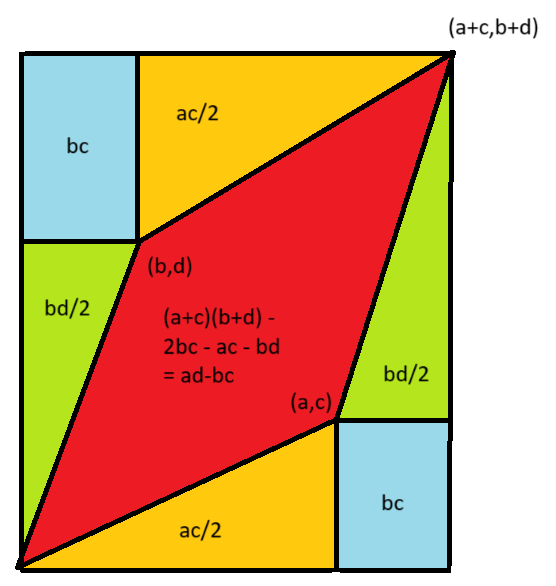
\includegraphics[width=100mm]{Images/img-2x2-det}
\caption{Visual proof of the area of a parallelogram made by vectors $\begin{pmatrix} a \\ c\end{pmatrix}$ and $\begin{pmatrix} b \\ d \end{pmatrix}$}
\label{fig-2x2-det}
\end{figure}

 In Figure \ref{fig-2x2-det}, the area of the red parallelogram is given by 
\[ (a+ b)(c+d)- 2bc-ac-bd=ad-bc\]

The \textit{sign} of $\det A$ is a bit mysterious, but what it does is tell us whether the area created by $u,v$ has been mirrored or not\footnote{With regards to our section about transformations of the plane, this means has the region been reflected in such a way that text is now backwards}. Specifically, if $\det A$ is negative, then the volume has been mirrored, and if $\det A>0$ then it has not. Taking absolute values $|\det A|$ tells you \textit{just} the area of this parallelogram\footnote{If you've taken Calc 3 this interpretation of the determinant should be familiar: Given a ``change of variables'' function $r=(x(u,v),y(u,v))$ the appropriate rescaling function for the double integral is the (absolute value of the determinant of the) Jacobian matrix \[ J=\begin{pmatrix} x_u & x_v \\ y_u & y_v\end{pmatrix}\] $|\det J|$ gives the amount that area has been skewed from $u,v$ coordinates into $x,y$ coordinate--for instance, the polar coordinate transformation $x(r,\theta) =  r\cos \theta, y(r,\theta)= r\sin \theta$ has Jacobian determinant of $r$}. 
%\begin{figure}
%	\[\includegraphics[width=120mm]{parallelogram}\]
%\end{figure}



\subsection{Determinants of $3\times 3$ matrices} You may recall the following formula for computing the determinant of a $3\times 3$ matrix\footnote{Perhaps from one interpretation of the calculation of the cross product of vectors $x,y\in\mathbf{R}^3$}
\begin{align} \label{eq-3x3-det} \det \begin{pmatrix} a & b & c \\ d & e & f \\ h & i & j\end{pmatrix} &= a\det \begin{pmatrix} e & f \\ i & j \end{pmatrix} - b \det \begin{pmatrix} d & f \\ h & j \end{pmatrix} + c \det\begin{pmatrix} d & e \\ h & i \end{pmatrix} \nonumber \\
&= a (ej-fi) - b(dj-fh)+c(di-eh) \nonumber \\
&= aej -afi +bfh-bdj +cdi -ceh
\end{align}
This funny looking expression tells us the same information for this $3\times 3$ matrix as it does for a $2 \times 2$ matrix. More specifically, \eqref{eq-3x3-det} computes the signed volume of the  formed by the column vectors \[ u=\begin{pmatrix} a \\ d \\ h \end{pmatrix}, \;  v=\begin{pmatrix} b \\ e \\ i \end{pmatrix},\;  w=\begin{pmatrix} c \\ f \\ j \end{pmatrix}\] in $\mathbf{R}^3$. If this volume is not 0, then the vectors $u,v,w$ must be linearly independent, and therefore the matrix $A$ represents a one-to-one function. Moreover, three linearly independent vectors must span $\mathbf{R}^3$, therefore the transformation represented by $A$ is also onto, and so $A$ must be invertible. 


\begin{terminology}
There's a funny word lurking in the previous example--\textbf{parallelepiped}. This is a real word, meaning ``sheared box of dimension $n$''. More specifically, a parallelepiped is the $n$-dimensional region created by ``closing up'' the box formed by $n$ vectors in $\mathbf{R}^n$. A specific example of a parallelepiped in $\mathbf{R}^3$ is given in Figure \ref{fig-piped}.

\begin{figure}[h!]
\centering 
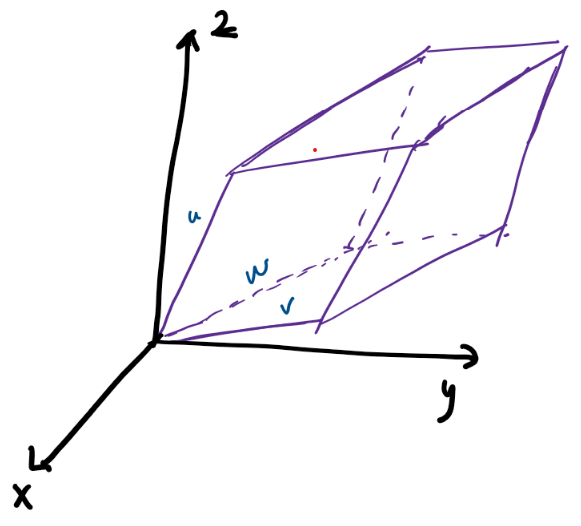
\includegraphics[width=70mm]{Images/img-piped}
\caption{The parallelepiped in $\mathbf{R}^3$ formed by vectors $u,v,w$}
\label{fig-piped}
\end{figure}

\end{terminology}

\subsection{Determinants in general}
Though there are some speedier algorithms for special cases, the most typical construction of the determinant of an $n\times n$ matrix is by an inductive process. That is to say, you can compute the determinant of an $n\times n$ in terms of determinants of its $(n-1)\times (n-1)$ submatrices, whose determinants are in turn computed by the determinants of their $(n-2)\times (n-2)$ matrices and so on\footnote{If you care about such things, the number of individual calculations needed to take the determinant is on the order of $n^3$ for an $n\times n$ matrix, the same as the number of calculations needed for row reduction to reduced echelon form.}. Eventually you get down to the $2\times 2$ submatrices, and just use equation \eqref{det-2x2}.

Let's start with the following geometric \textit{definition} of the determinant. 

\begin{defn}
	Let $A$ be an $n\times n$ matrix and $a_1,\cdots, a_n$ be the column vectors of $A$. Then $\det A$ is the real number equal to the signed hypervolume of the parallelopiped formed by vectors $a_1,\cdots,a_n\in \mathbf{R}^n$.
\end{defn}

\begin{remark}$\det$ then defines a function \begin{equation} \det \colon \{ \text{$n\times n$ matrices}\} \to \mathbf{R}\end{equation}
You may also see people write $|A|$ for the determinant of $A$. Since these kind of vertical bars are already vastly overused, we'll stick with $\det$. \end{remark}
Note that this definition doesn't necessarily give us the means to compute the determinant just yet. That comes into play in the following section. I leave it to you to convince yourself of the following: 

\begin{thm}
	Let $A$ be an $n\times n$ matrix. Then $A$ is invertible if and only if $\det A\neq 0$ 
\end{thm}
\begin{remark}This is another thing to add to the list from Theorem \ref{thm-inv-matrix-1}.\end{remark}

\subsection{Computing the determinant}
The most common algorithm for computing the determinant of a matrix is called \textit{cofactor expansion}. We need some definitions: 

\begin{defn}For an $n\times n$ matrix $A$, let $A_{i.j}$ denote the $(n-1)\times (n-1)$ matrix obtained from $A$ by deleting row $i$ and column $j$ from $A$. This matrix $A_{i,j}$ is called the \textbf{cofactor} to the entry $a_{i,j}$ in $A$.
\end{defn} 

Let's let $S$ be the $n\times n$ ``matrix of signs" as follows
\begin{equation} S=\begin{pmatrix} 
+ & - & + & - & \cdots & \\ 
- & + & + & \ddots && \\
+ & - & \ddots &&& \\
- & \ddots &&&& \\
\vdots &&&&\\
&&&&&
\end{pmatrix}\end{equation}
Note that the $i,j$ entry of $S$ is just $(-1)^{i+j}$. The \textbf{cofactor expansion} of $\det A$ along row\footnote{You can also calculate the determinant by cofactor expansion along a \textit{column} of $A$} $i$ is then the sum
\begin{equation} \label{eqn-cof-i}
	 \sum_{j=1}^n (-1)^{i+j} a_{i,j} \det A_{i,j} 
\end{equation}

\begin{thm}
	For $A$ an $n\times n$ matrix, $\det A$ is computed by cofactor expansion \eqref{eqn-cof-i} along any row of $A$. 

\end{thm}

A good strategy for computing the determinant of a big matrix $A$ is to use cofactor expansion along the row which contains the most zeros. 

Note that if $n=3$ this exactly the computation from \eqref{eq-3x3-det}. Moreover, computing the determinant of a matrix (in this way at least) is an inductive process: you repeatedly apply cofactor expansion until you reduce your calculation to $2\times 2$ matrices, then use equation \eqref{det-2x2}. There are other ways of calculating the determinant, but this is the simplest to describe and needs the least additional terminology\footnote{One such way to calculate the determinant is as a sum over the elements of the $n$-th symmetric group (the collection of all permutation of the set $\{1,2,3,\cdots, n\}$), another (much more sophisticated way) is as an alternating $n$ form, they all do the same thing.}.

\subsection{Properties of the determinant}
We've now introduced a new tool, the determinant, to our world of matrices. It remains to see how this interacts with the operations on matrices we've already seen. A useful proposition is the following:

\begin{prop}
Let $A,B$ be $n\times n$ matrices. Then the following hold:
\begin{enumerate}
	\item $\det(AB)=\det(A)\det(B)$
	\item $\det(A^T)=\det A$
	\item If $A$ is invertible, $\det(A^{-1})=1/\det A$
\end{enumerate}
\end{prop}
\begin{proof}[``Proof"]
Part a. is proved by showing that elementary row operations are (i) represented by matrices and (ii) have the multiplicative property on determinants. This is what is shown in Proposition \ref{prop-elm-mat}, to really show this rigorously requires a technique called \textit{mathematical induction}. Part b. follows in that cofactor expansion along a \textit{column} also calculates the determinant (you can check this). For part c., note that $AA^{-1}=I$. Using part a we have \[\det(A)\det(A^{-1})=\det(AA^{-1})=\det(I)=1\] so that $\det (A^{-1})=1/\det A$. 
\end{proof}

In general, you do not expect that the determinant should respect addition of matrices, that is: \[ \det (A+B)\neq \det A+\det B\]
A good thing to check is how elementary row operations interact with the determinant. I leave it to you to check the following (there are some exercises that show this in special cases):

\begin{prop}[Row operations and the determinant] \label{prop-elm-mat} Let $A$ be a square matrix. Then the following hold:
\begin{enumerate}
	\item If $B$ is obtained by multiplying a row of $A$ by $k$ then $\det B=k\det A$
	\item If $B$ is obtained by adding a row to another row within $A$ then $\det B=\det A$
	\item If $B$ is obtained by permuting $\ell$ rows of $A$ then $\det B=(-1)^{\ell}\det A$. 
\end{enumerate}
\end{prop}







\subsection{Exercises}
\begin{enumerate}[label=\arabic*.]

\item Compute the determinant of the following matrices
\begin{enumerate}
	\item $\begin{pmatrix} 3 & 0 & 4 \\ 2 & 3 & 2 \\ 0 & 5 & -1  \end{pmatrix}$
	\item $\begin{pmatrix} 1 & -2 & 4 & 2 \\ 0 & 0 & 3 & 0 \\ 2 & -4 & -3 & 5 \\ 2 & 0 & 3 & 5\end{pmatrix}$
	\item $\begin{pmatrix} 3 & 0 & 0 & 0 \\ 7 & -2 & 0 & 0 \\ 2 & 6 & 3 & 0 \\ 3 & -8 & 4 & -3  \end{pmatrix}$
	\item $\begin{pmatrix} 6 & 0 & 2 & 4 & 0 \\ 9 & 0 & -4 & 1 & 0  \\ 8 & -5 & 6 & 7 & 1 \\ 2 & 0 & 0 & 0 & 0 \\ 4 & 2 & 3 & 2 & 0 \end{pmatrix}$
\end{enumerate}

\item An (upper\footnote{There are also lower triangular matrices, a matrix is \textit{lower triangular} if its transpose is upper triangular.}) \textbf{triangular matrix} is any $n\times n$ matrix of the form \[ A=\begin{pmatrix} a_{1,1} & * & * & \cdots & * \\
0 & a_{2,2} & * & \cdots & * \\
0 & 0 & a_{3,3} & \cdots & * \\
\vdots & \vdots  & \vdots & \ddots & \vdots \\
0 & 0 & 0 & \cdots & a_{n,n} \end{pmatrix}\]
where the diagonal entries $a_{i,i}\neq 0$, 0s below the main diagonal, and the entries marked $*$ are any real number. Show that the determinant of a triangular matrix is given by \[ \det A= a_{1,1} a_{2,2} \cdots a_{n,n}\]
Are triangular matrices invertible? 

\item Let $R_{\theta}=\begin{pmatrix} \cos \theta & -\sin\theta \\ \sin \theta & \cos \theta\end{pmatrix}$. Show that $\det R_{\theta}=1$. 
\item Let $B=\begin{pmatrix} 1 & 0 & 1 \\ 1 & 1 & 2 \\ 1 & 2 & 1 \end{pmatrix}$, compute $\det(B^4)$. 
\item Show that $\det (kA)=k^n \det A$ for $A$ an $n\times n$ matrix and $k$ a scalar. Is $\det$ a linear transformation $\mathbf{R}^{n^2}\to\mathbf{R}$?

\item Show that $\det(A+B)\neq \det A+\det B$ by producing a pair of matrices for which the equation does not hold.
 
\item A matrix $A$ is called \textbf{symmetric} if $A^TA=I$. Show that $\det A=\pm 1$ for any symmetric matrix $A$.

\item Compute the determinants of the following $3\times 3$ matrices in terms of $k$
\begin{enumerate}
	\item $\begin{pmatrix} 1 & 0 & 0 \\ 0 & 1 & 0 \\ 0 & k & 1\end{pmatrix}$
	\item $\begin{pmatrix} 0 & 1 & 0 \\ 1 & 0 & 0 \\ 0 & 0 & 1\end{pmatrix}$
	\item $\begin{pmatrix} 0 & 1 & 0 \\ 0 & 0 & 1 \\ 1 & 0 & 0\end{pmatrix}$
	\item $\begin{pmatrix} k & 0 & 0 \\ 0 & 1 & 0 \\ 0 & 0  & 1\end{pmatrix}$

\end{enumerate}

\item \textit{True or False}. Determine if the following statements are true or false. Justify your answer
\begin{enumerate}
	\item If $A=(a_1 \cdots a_n)$ such that the collection of vectors $a_1, \cdots, a_n\in\mathbf{R}^n$ is linearly dependent, then $\det A=0$
	\item If $A=\begin{pmatrix} a & b \\ c & d\end{pmatrix}$ such that $a,b,c,d$ are all real numbers in the interval $[-1,1]$, then it is not possible that $\det A=3$. 
	\item If $A$ is an $n\times n$ matrix such that $\det(A^3)=0$ then $A$ is not invertible
	\item For any invertible matrix $P$, $\det(PAP^{-1})=\det(A)$. 
	\item If $A=\begin{pmatrix} a & b \\ c & d\end{pmatrix}$ such that $a,b,c,d\geq 0$ then $\det A\geq 0$.
	\end{enumerate}

\item *The notation $\GL{n}$ is often used to denote the set\footnote{It's actually a \textit{group}, actually it's a \textit{Lie group}} of $n\times n$ invertible matrices (with real coefficients), and $\SL{n}$ is used to denote the subset of such matrices $A\in \GL{n}$ with $\det A=1$. Show that if $A,B\in \SL{n}$ then $A^{-1}\in \SL{n}$ and $AB\in \SL{n}$. 

Some terminology:  ``GL'' means \textit{general linear}, and ``SL'' means \textit{special linear}.

\item *Recall the matrix representations of the elementary row operations from 
\begin{enumerate}
	\item Show that $\det E_{i,j}=1, \det R(i,k)=k$ and $\det S(i,j)=(-1)^{i+j}$
	\item Conclude that an elementary row operation applied to $A$ does not affect whether or not $A$ is invertible 
	\item If the rows of $A$ are linearly independent then $\det(A)\neq 0$.
	\end{enumerate}
\end{enumerate}

Additional suggested exercises: \textit{Lay} sections 3.1, 3.2



\section{Vector spaces} 

So far, we've been using our intuition of vectors as ``arrows'' in $n$-dimensional (Euclidean) space. However, math is built on abstraction, and linear algebra is a great example of a subject where the tools we build apply in a much more general setting. 

\begin{defn}A \textbf{vector space}\footnote{In this class, all of our vector spaces are over $\mathbf{R}$, but more correct is to say ``vector space over $\mathbf{R}$" here. This means the scalars come from the \textit{field} $\mathbf{R}$. Sometimes it's necessary to consider vector spaces over $\mathbf{C}$, the field of complex numbers,  $\mathbf{Q}$ the field of rational numbers, or \textit{finite fields} like the integers modulo a prime number $p$} is a set $X$ whose elements are things called \textit{vectors} and which act like vectors that we've been working with so far. That is to say, the following axioms are all satisfied
\begin{enumerate}
	\item If $x,y\in X$ then there is a vector $x+y\in X$
	\item For all $x,y,z\in X$; $x+y=y+x$ and $(x+y)+z=x+(y+z)$
	\item If $x\in X$, $k\in\mathbf{R}$ a scalar there is a vector $kx\in X$
	\item There is a vector $\vec{0}\in X$ such that $x+\vec{0}=\vec{0}+x=x$ for all $x\in X$
	\item Given $x\in X$ there is a vector $-x\in X$ such that $x+(-x)=\vec{0}$
	\item For any vectors $x,y\in X$, scalars $k\in\mathbf{R}$; $k(x+y)=kx+ky$
	\item For any vector $x\in X$ and scalar $k,\ell\in\mathbf{R}$; $(k+\ell)x=kx+\ell x$ and $(k\ell)x=k(\ell x)$
	\item For any vector $x\in X$, $0x=\vec{0}$. 
\end{enumerate}
\end{defn}

\begin{example} Examples are always necessary: 

\begin{itemize}
\item The space $\mathbf{0}$ consisting of a single vector $\vec{0}$ (the zero vector) is a vector space. We call this the \textbf{trivial vector space}. You could also \textit{define} $\mathbf{R}^0$ to be this space. 

\item An assuring fact is that the sets $\mathbf{R}^n$ for $n\geq 1$ we've been working with so far are vector spaces. You can think of these as the ``geometric'' vectors, in that elements in $\mathbf{R}^n$ \textit{can} (but don't have to) be interpreted as arrows in $n$-dimensional space. 

\item Let $C(\mathbf{R})$ denote the set of continuous functions $f\colon\mathbf{R}\to\mathbf{R}$. Then $C(\mathbf{R})$ is a vector space, with operations defined as \[ (f+g)(x)=f(x)+g(x), \quad (kf)(x)=kf(x)\] for $f,g\in C(\mathbf{R})$ and $k$ a scalar. The difference with this function space is that is it not a finite-dimensional vector space, therefore understanding elements of this vector space is more nuanced\footnote{For instance, if you recall Taylor series from calculus, this is essentially asking what functions can be represented in terms of the basis $\{x^k\}_{k\geq 0}$ of monomials. A similar idea underlies Fourier analysis where you seek to represent (periodic) functions in terms of $\sin(kx)$ and $\cos(kx)$. Not to mention that linear transformations are no longer necessarily given by matrices.}. 

\item Let $M(m,n)$ be the set of $m\times n$ matrices. Then $M(m,n)$ is a vector space with operations defined as in \eqref{eq-add-mat}. $M(m,n)$ is an $mn$ dimensional vector space, a choice of basis would be the collection of all matrices with just one entry of 1, and all other entries 0\footnote{Something worth checking is that such a matrix is the \textit{external product} of basis vectors $e_ie_j^T$}. Note that as a set $M(m,n)$ is just $\mathbf{R}^{mn}$, the difference is in how we choose to interpret such objects. 

%\item 

\end{itemize}
\end{example}

\subsection{Subspaces and bases}
We've used words like \textit{span} and \textit{spanning set} a lot so far. More general is to talk about subspaces and bases. 

\begin{defn} Given a vector space $X$ a \textbf{subspace} is a subset $V\subset X$ such that: 
\begin{enumerate}
	\item If $u,v\in V$ then $u+v\in V$
	\item If $v\in V$ and $k$ a scalar, then $kv\in V$
\end{enumerate}
\end{defn}

Said differently, a subspace $V\subset X$ is just another vector space which lives naturally inside the bigger space $X$. Any span of vectors in $\mathbf{R}^n$ is a subspace of $\mathbf{R}^n$. Note as well that this means the zero vector $\vec{0}=0v$ must be contained in any subspace of $X$. Any vector space $X$ has the two $\{\vec{0}\}$ and the whole space $X$. We call $\{\vec{0}\}$ the \textbf{trivial} subspace. 

The main fact about subspaces is that they must always be given as the span of a (finite) collection of vectors. Given a subspace $V\subset\mathbf{R}^n$ we use the term \textit{basis} to refer to any linearly independent spanning set of $V$, as follows:

\begin{defn}Let $X$ be a vector space and  $V\subset X$ be a subspace of $X$. A collection of vectors $v_1,\cdots,v_k\in V$ is called a \textbf{basis} of $V$ if following two conditions are met
\begin{enumerate}
	\item The vectors $v_1,\cdots,v_k$ are linearly independent
	\item $\Span{v_1,\cdots, v_k}=V$
\end{enumerate}
\end{defn}

Note that a subspace $V\subset X$ may have many bases, but they must all consist of the same number of vectors. A subspace $V$ is said to have \textbf{dimension} $k$ if it has a basis consisting of $k$ vectors. In particular, since $\mathbf{R}^n$ has the standard basis $e_1,\cdots,e_n$, $\mathbf{R}^n$ is a vector space of dimension $n$. For a vector space $X$ let's write $\dim X$ for the dimension of $X$. 



\subsection{Canonical subspaces of a marix/linear transformation}

Given a linear transformation $T\colon \mathbf{R}^n\to\mathbf{R}^m$ represented by $m\times n$ matrix $A$, there are many canonical subspace of the domain and range associated to $T$. 

\begin{itemize}
	\item The \textbf{nullspace} of $A$, written $\nul{A}$, is the set of vectors $x\in\mathbf{R}^n$ such that $Ax=\vec{0}$. This is the same as the \textbf{kernel} of $T$, i.e., the set $\ker T$ of vectors $x\in\mathbf{R}^n$ such that $T(x)=\vec{0}$.
	\item The \textbf{column space} of $A$, written $\col{A}$, is the set of vectors $b\in\mathbf{R}^m$ such that $Ax=b$ for some $x \in \mathbf{R}^n$. Note that $\col{A}$ is the same as the span of the columns of $A$, and so is the same as the image of the transformation $T$.
	\item The \textbf{row space} of $A$, written $\row{A}$, is the span of the rows of $A$. 
\end{itemize}

\begin{prop}
	Given $m\times n$ matrix $A$, the sets $\nul{A}$ and $\row{A}$ are subspaces of $\mathbf{R}^n$, the set $\col{A}$ is a subspace of $\mathbf{R}^m$. Moreover, $\col{A^T}=\row{A}$ and $\row{A^T}=\col{A}$.
\end{prop}

\begin{proof}
	We'll show that $\nul{A}\subset \mathbf{R}^n$ is a subspace. Suppose that $x,y\in \nul{A}$, then $Ax=Ay=\vec{0}$. So, $A(x+y)=Ax+Ay=\vec{0}+\vec{0}=\vec{0}$. Similarly, if $x\in \nul{A}$ and $k$ a scalar, then $A(kx)=k(Ax)=k\vec{0}=\vec{0}$. Therefore $\nul{A}$ is a subspace.
	
	Next let's show that $\col{A}$ is a subspace of $\mathbf{R}^m$. Suppose that $u,v\in \col{A}$. Then there are $x,y\in\mathbf{R}^n$ with $Ax=u$ and $Ay=v$. Therefore $u+v=Ax+Ay=A(x+y)$, and so $u+v\in \col{A}$. Further, if $k$ a scalar then $ku=k(Ax)=A(kx)$ so that $ku\in \col{A}$. 
	
	The remainder is left as an exercise. 
\end{proof}

\begin{example}[A basis for the nullspace of $A$]
	Using the techniques of Section \ref{sec-hom} we can produce a canonical basis for the nullspace of $A$. First, find the matrix $B$ such that $A\sim B$ and $B$ is in reduced echelon form. Then you can read off the vectors associated to any free variable in the solution set of $Bx=\vec{0}$. Since $A\sim B$ if and only if $A=EB$ for $E$ some product of elementary matrices. Since $E$ is then invertible, $E^{-1}$ exists and so the solution sets to $Ax=\vec{0}$ and $Bx=E^{-1}\vec{0}=\vec{0}$ must be the same.

\end{example}


\begin{terminology} 
	The dimensions of these canonical spaces also have names associated to them: 
	\begin{itemize}
		\item The dimension of $\nul{A}$ is called the \textbf{nullity} of $A$.
		\item The dimension of $\col{A}$ is called the \textbf{column rank} of $A$. We denote by $\rank{A}$ the \textit{column} rank of matrix $A$. The unadjectivized word "rank" typically refers to column rank of a matrix.
		\item The dimension of $\row{A}$ is called the \textbf{row rank} of $A$.
	\end{itemize}
	If $A$ is a matrix representation of a linear transformation $T$ then these words just as well apply to $T$: for instance, the nullity of $T$ is the dimension of $\nul{A}$. 
\end{terminology}

\subsection{Rank-nullity theorem} 
The big theorem for this section is something that we've seen before but haven't yet written down fully. 

\begin{thm}[Rank-nullity theorem]
	Let $A$ be an $m\times n$ matrix. Then \begin{equation} \dim(\col{A})+\dim(\nul{A})=n\end{equation}
\end{thm}

Said differently, the dimension of the domain of a linear transformation represented by an $m\times n$ matrix $A$ is always the sum of the dimension of the nullspace of $A$ plus the dimension of the column space of $A$. 

\begin{proof}
This theorem follows from the general fact that any matrix is row equivalent to one of reduced echelon form: If $A$ is in reduced echelon form then a column of $A$ 
\begin{itemize}
	\item Contains a leading 1, in which case it is counts toward the dimension of the column space
	\item Does not contain a leading 1, in which case it will count toward a free variable when parametrizing the nullspace of $A$.
\end{itemize}
Here's the trick though: Suppose $A$ not in echelon form and write $B$ for its reduced echelon form. Then the column spaces of $A$ and $B$ need not be the same. They are, however, isomorphic\footnote{If $A=EB$ for $E$ a product of elementary matrices, then $Ax=b$ if and only if $Bx=E^{-1}b$. Since $E$ is invertible, the map $b\mapsto E^{-1}b$ from $\col{A}\to\col{B}$ is an isomorphism.}, and so $\dim{\col{A}}=\dim{\col{B}}$. 
\end{proof}

In terms of the transformation $T$ between (finite dimensional) vector spaces $T\colon X\to Y$, that \[ \dim X=\dim (\ker T)+\dim(\img T)\]


\subsection{Isomorphisms}
Consider the subspace $V=\Span{ \begin{pmatrix} 1 \\ 2 \\ 0 \end{pmatrix}, \begin{pmatrix} -1 \\ 0 \\ 3\end{pmatrix}}$ of $\mathbf{R}^3$. Since geometrically, $V$ is a plane through the origin, it's tempting to say that $V$ is ``$\mathbf{R}^2$" sitting inside of $\mathbf{R}^3$---but that's not correct. When talking about subspaces (or vector spaces in general) that functionally are the same as something more canonical, the right term to use is \textit{isomorphic}\footnote{\textit{Iso}- from Greek meaning ``same", \textit{morph} from Greek meaning ``shape"}. 

\begin{defn}Let $X,Y$ be vector spaces. A linear transformation $T\colon X\to Y$ is called an \textbf{isomorphism} if it is both one-to-one and onto. \end{defn}
If $X,Y$ are vector spaces such that there is an isomorphism $T\colon X\to Y$ then $X$ and $Y$ are called \textbf{isomorphic}. In notation we write $X\cong Y$. 

\begin{fact}
If $V\subset \mathbf{R}^n$ is a subspace then $V\cong \mathbf{R}^k$ for some $k\in \{0,1,2,\cdots,n\}$\footnote{An even more general fact is that if $V$ is \textit{any} vector space then $V\cong \mathbf{R}^{\alpha}$ for some cardinal number $\alpha$. For instance if the vector space $C(\mathbf{R})$ of continuous functions is isomorphic to $\mathbf{R}^{\infty}$ where $\infty$ denotes the smallest infinite cardinal number (sometimes called ``countable infinity"). There's an (easy) proof of this using the most controversial axiom in all of mathematics---\textit{the axiom of choice}. While this result seems underwhelming it basically tells you that you are free to think of vector spaces as always coming equipped with a choice of basis, sometimes we need to change this basis, but existence of a basis can always be assumed}.
\end{fact}

\begin{remark}
	Using the term \textit{isomorphic} is an important distinction for vector spaces. Addressing the question from earlier, the subspace \[V=\Span{ \begin{pmatrix} 1 \\ 2 \\ 0 \end{pmatrix}, \begin{pmatrix} -1 \\ 0 \\ 3\end{pmatrix}}\] is not \textit{equal} to $\mathbf{R}^2$ because the elements in the two are different. However, from the perspective of linear algebra, the distinction between them is purely semantic: they behave as the same object (you can think of $V$ as a ``copy" of $\mathbf{R}^2$ inside $\mathbf{R}^3$ with coordinates given by the basis). The way to express this mathematically is to that $V$ is isomorphic to $\mathbf{R}^2$. Said differently, isomorphisms are the right notion of ``equality" for vector spaces\footnote{This might feel uncomfortable at first but you have some experience with this type of language already: for instance, are the numbers $\frac{1}{2}$ and $\frac{3}{6}$ the same? They can both be reduced to the same fraction so the answer must be yes, but they are not literally the same fraction. You can say that fractions $\frac{p}{q}$ and $\frac{r}{s}$ are ``equal" if and only if $sp=qr$.}. 
	
	In fact, any finite dimensional vector space is  isomorphic to $\mathbf{R}^n$ for some $n\geq 0$, therefore, we're really not losing any generality by just looking at such vector spaces. 
\end{remark}

\subsection{Exercises}
\begin{enumerate}[label=\arabic*.]
	\item Let $A$ be the following matrix \[ A=\begin{pmatrix} 1 & 4 & 8 & -3 & -7 \\ -1 & 2 & 7 & 3 & 4\\ -2 & 2 & 9 & 5 & 5 \\ 3 & 6 & 9 & -5 & -2\end{pmatrix}\] 
	Write a basis for $\nul{A}$ and for $\col{A}$. 
	
	\item Write a basis for the subspace of $\mathbf{R}^n$ 
	\begin{enumerate}
		\item  $\Span{ \begin{pmatrix} 1 \\ -1 \\ -2 \\ 5\end{pmatrix}, \begin{pmatrix} 2 \\ -3 \\ -1 \\ 6 \end{pmatrix}, \begin{pmatrix} 0 \\ 2 \\ -6 \\ 8 \end{pmatrix}, \begin{pmatrix} -1 \\ 4 \\ -7 \\ 7 \end{pmatrix}, \begin{pmatrix} 3\\ -8 \\ 9 \\ -5 \end{pmatrix}}$
		\item The set of vectors $v\in \mathbf{R}^7$ such that $v_1=0$
		\item The set of vectors $v\in \mathbf{R}^5$ such that $Av=\vec{0}$ for $A$ the matrix \[ A=\begin{pmatrix} 1 & 1 & 1 & 0 & 0 \\ 0 & 0 & 0 & 1 & 1\end{pmatrix}\]
	\end{enumerate}	
	\item Let $V\subset \mathbf{R}^3$ be the subset of vectors $\begin{pmatrix} x \\ y \\z\end{pmatrix}$ such that $x+y+z=0$
	\begin{enumerate}
		\item Show that $V$ is a subspace of $\mathbf{R}^3$.
		\item Show that $\left\{ \begin{pmatrix} 1 \\ -1 \\ 0 \end{pmatrix} , \begin{pmatrix} 0 \\ 1 \\ -1\end{pmatrix}\right\}$ is a basis for $V$
		\item Let $W$ be the subset of vectors of $\mathbf{R}^3$ such that $x+y+z=1$. Is $W$ still a subspace of $\mathbf{R}^3$? Explain why or why not. 	
	\end{enumerate}
	
	\item Determine if the following is a subspace of the given vector space
	
	\begin{enumerate}
		\item The set of matrices $A\in M(m,n)$ such that $\det A=0$.
		\item The set of continuous functions $f\in C(\mathbf{R})$ such that $f(0)=0$.
		\item The set of continuous functions $f\in C(\mathbf{R})$ such that $f(0)=1$
		\item The set of continuous functions $f\in C(\mathbf{R})$ such that $\lim_{x\to \infty} f$ exists.
	\end{enumerate}
	
	\item The \textbf{trace} of an $n\times n$ matrix $A$, denoted $\tr{A}$, is the sum of the diagonal entries from $A$. That is, \[ \tr{A}=a_{1,1}+a_{2,2}+\cdots+a_{n,n}.\]
		Show that the set of matrices $A\in M(n,n)$ of trace $0$ is a subspace of $M(n,n)$.
	
	\item  Here are even \textit{more} entries to the invertible matrix theorem (Theorem \ref{thm-inv-matrix-1}). Show that the following are equivalent to a matrix $A$ being invertible \begin{enumerate}\setcounter{enumii}{14}
		\item The columns of $A$ form a basis for $\mathbf{R}^n$
		\item $\col{A}\cong \mathbf{R}^n$.
		\item $\rank{A}=n$
		\item $\dim \nul{A}=0$
		\item $\nul{A}\cong \mathbf{0}$. 
	\end{enumerate}
	
	\item Let $u=\begin{pmatrix} 1 \\ -4 \end{pmatrix}, v=\begin{pmatrix} -2 \\ 7\end{pmatrix}$.
	\begin{enumerate}
		\item Show that $\{u,v\}$ is a basis for $\mathbf{R}^2$. 
		\item Let $B=\begin{pmatrix} u & v\end{pmatrix}$. Determine $B^{-1}$.
		\item Let $T$ be the linear transformation given by $Te_1=\begin{pmatrix} 1 \\ 3\end{pmatrix}, Te_2=\begin{pmatrix} 0 \\ -3\end{pmatrix}$. Then the standard matrix representation of $T$ is given by $A=\begin{pmatrix} 1 & 0 \\ 3 & -3\end{pmatrix}$. The matrix $BAB^{-1}$ is called the \textit{conjugate} of $A$ by $B$, and represents the transformation $T$ with respect to the basis $\{u,v\}$. Use this to evaluate $T(3u+2v)$
	\end{enumerate}

	\item Give an example of a $4\times 3$ matrix $A$ with $\rank{A}=1$, or explain why no such matrix exists. 

	\item Is the following a basis for $M(2,2)$? Explain why or why not (if not, describe the subspace of $M(2,2)$ formed by $\mathcal{B}$)\[\mathcal{B}= \left\{T= \begin{pmatrix} 1 & 1 \\ 0 & 0 \end{pmatrix}, B=\begin{pmatrix} 0 & 0 \\ 1 & 1 \end{pmatrix}, L=\begin{pmatrix} 1 & 0 \\ 1 & 0 \end{pmatrix}, R=\begin{pmatrix} 0 & 1 \\ 0 & 1 \end{pmatrix}\right\}\] 


	

	
	\item True or False. Determine if the following statements are true or false. Justify your answer.
	\begin{enumerate}
		\item If $A$ is in reduced echelon form $\rank{A}$ is equal to the number of columns with leading 1s
		\item If $A\sim B$ by row operations then $\nul{A}\cong \nul{B}$ and $\col{A}\cong \col{B}$
		\item There is a $3\times 4$ matrix $A$ with both nullity and (column) rank 2
		\item If $A$ is a $5\times 7$ matrix then $\nul{A}$ can have dimension $0$	
		\item If $\{v_1,\cdots,v_n\}$ is a basis of $\mathbf{R}^n$ and $T\colon \mathbf{R}^n\to\mathbf{R}^n$ an invertible linear transformation then $\{Tv_1,\cdots,Tv_n\}$ is also a basis of $\mathbf{R}^n$. 
		\item If $\{v_1,\cdots,v_n\}$ is a basis of $\mathbf{R}^n$ and $T\colon \mathbf{R}^n\to\mathbf{R}^m$ \textit{any} linear transformation then $\{Tv_1,\cdots,Tv_n\}$ is a basis of $\mathbf{R}^m$. 
		\item *For $A$ an $m\times n$ matrix, $\dim(\row A)=\dim(\null A)$
	\end{enumerate}
	
	
	\item Let $T\colon M(2,2)\to M(2,2)$ (the collection of $2\times 2$ matrices) be given by $T(A)=A+A^T$. 
	\begin{enumerate}
		\item Show that $T$ is a linear transformation
		\item Describe the kernel and image of $T$
	\end{enumerate}
	
		\item *Define $T\colon C(\mathbf{R})\to C(\mathbf{R})$ by $T_f$ is the function given by \[ T_f(x)=\int_0^x f(t)\,dt\]
	\begin{enumerate}
		\item Show that $T$ is a linear transformation
		\item Describe the kernel of $T$
	\end{enumerate}
	

	\item *Let $P_n$ denote the set of (real) polynomials of degree at most $n$
	\begin{enumerate}
		\item Show that $P_n$ is a subspace of $C(\mathbf{R})$. 
		\item Show that $P_n\cong \mathbf{R}^{n+1}$
		\item Is $\{1+x^2, 1-x^2\}$ a basis for $P_2$? Explain why or why not (if not, give an example of another element that must be added to make it a basis).  
		\item Show that $D\colon P_n\to P_{n-1}$ given by $D(f)=f'$ (the derivative) is a linear transformation, and describe $\ker D$.
	\end{enumerate} 
	
\end{enumerate}

Suggested additional exercises: \textit{Lay} sections 4.1, 4.2, 4.3



\section{Eigenvalues and eigenvectors}

To understand a linear transformation $T$ on $\mathbf{R}^n$, it's often useful to understand what (if any) features of the domain are unchanged by $T$. Historically, this idea comes (in part) from studying rotations of a solid object in $\R^3$. Any such rotation must have a fixed axis\footnote{This is sometimes called Euler's rotation theorem}, which is also the axis of rotation. Knowing this fixed axis gives information about the rotation, and vice verse. More generally, linear transformations have what are called \textit{eigenvalues} and \textit{eigenvectors}, which characterize the transformation independent of choice of basis.   %For instance, one observation is that any linear transformation $T$ on $\mathbf{R}^3$ has a dimension one subspace (line) which is unchanged by $T$ (see Exercise \ref{princ-axis}). As it turns out, understanding such ``fixed axes" of $T$, gives us deep insight into the structure of linear transformations. Let's begin with a definition.


\begin{defn}[Eigenvalue and eigenvector]Let $T$ be a linear transformation $\mathbf{R}^n\to\mathbf{R}^n$. A number $\lambda\in\mathbf{R}$ is called an \textbf{eigenvalue}\footnote{This somewhat funny looking word comes from the root \textit{eigen}- in German, which means ``own'' or ``self".} of $T$ if there is a nonzero vector $x\in\mathbf{R}^n$ such that \begin{equation} \label{eigenvalue} T(x)=\lambda x\end{equation}
Given an eigenvalue $\lambda$ of $T$, any vector $x$ such that equation \eqref{eigenvalue} holds is called an \textbf{eigenvector} (for that {eigenvalue}) of $T$. 
\end{defn}


\subsection{The characteristic polynomial} 
Let's determine how to find eigenvalues of a linear transformation. Note that if $\lambda$ is an eigenvalue of $T$ then there is nonzero vector $x$ such that 
\begin{equation} T(x)-\lambda x=(T-\lambda I)x=\vec{0} \end{equation}
(recall that $I$ is the identity function on $\mathbf{R}^n$.) That is to say, that $\lambda$ is a number such the linear transformation $T-\lambda I$ has a nonzero vector in its kernel, therefore is not one-to-one, and so is not invertible. This is the same as any matrix representation of $T-\lambda I$ not being an invertible matrix. Suppose that $T(x)=Ax$ for some $n\times n$ matrix, $A$. If $\lambda$ is an eigenvalue of $T$, then the matrix $A-\lambda I$ must not be invertible. Since one (of many) equivalent condition for a matrix to be noninvertible is to have determinant of zero, we have the following observation: 

\begin{fact}
	If $T\colon\mathbf{R}^n\to\mathbf{R}^n$ is given by $T(x)=Ax$ for some $n\times n$ matrix $A$. Then $\lambda$ is an eigenvalue for $T$ if and only if $\det(A-\lambda I)=0$.
\end{fact}

\begin{example}\label{ex-eigen}Let's consider the transformation $T\colon\mathbf{R}^2\to\mathbf{R}^2$ given by $T(x)=Ax$ for $A$ the matrix \begin{equation} A=\begin{pmatrix} 3 & 1 \\ 6 & -2\end{pmatrix}\end{equation} 
Calculating, we have \[ \det(A-\lambda I)=\det \begin{pmatrix} 3 -\lambda & 1 \\ 6 & -2-\lambda \end{pmatrix} = (3-\lambda)(-2-\lambda)-6=\lambda^2-\lambda -12\]


Since $\lambda^2-\lambda -12=(\lambda -4)(\lambda+3)$ we've found that $A-\lambda I$ is not invertible if and only if $\lambda=4$ or $\lambda=-3$. 

\end{example}
In the above example, we found that $\det(A-\lambda I)$ was a polynomial in the variable $\lambda$. It's worth convincing yourself that this will generally be true. Since it contains information about eigenvalues, let's give this polynomial a name.

\begin{defn}
	Let $T\colon \mathbf{R}^n\to\mathbf{R}^n$ be a linear transformation with standard matrix representation given by $n\times n$ matrix $A$. The \textbf{characteristic polynomial} of $T$, denoted $\chi$ is the polynomial given by \begin{equation} \chi(\lambda)= \det(A-\lambda I)\end{equation}
\end{defn}

It's appropriate to call $\chi$ the characteristic polynomial of the matrix $A$ as well, and often more useful since this is how we calculate $\chi$. If possible unclear, we'll write $\chi_A$ to denote that $\chi$ is the characteristic polynomial of the $n\times n$ matrix $A$. Note that since $\lambda$ is a eigenvalue of $T$ if and only if $\det(A-\lambda I)=0$, we have the following fact: 

\begin{fact} $\lambda$ is an eigenvalue of the transformation $T\colon x\mapsto Ax$ if and only if $\lambda$ is is a root of the characteristic polynomial of $A$. 
\end{fact}

\begin{remark}
	Note that $\det(A-\lambda I)$ is a polynomial in $\lambda$ of degree at most $n$. A fact you may recall from algebra is that any degree $n$ polynomial (with coefficients that are real numbers) has at most $n$ distinct roots\footnote{This is a corollary of the \href{https://en.wikipedia.org/wiki/Fundamental_theorem_of_algebra.}{Fundamental theorem of algebra}}. In particular, any such polynomial will factor as a product of (i) linear factors, or (ii) irreducible quadratic factors. That is to say, a linear transformation on $\mathbf{R}^n$ can have at most $n$ different eigenvalues. 
	
	%It's useful the to understand how this fact about polynomials, when applied to the characteristic polynomial of a linear transformation, can give us information about the transformation itself.
\end{remark}	


\subsection{Eigenspaces}
Note that if $\lambda$ is an eigenvalue for $T$, and $x$ a corresponding eigenvector, then $T$ ``fixes'' the subspace of $\mathbf{R}^n$ given by the span of $x$. That is, since $T$ acts by scalar multiplication on this subspace, the action of $T$ on this subspace is particularly simple.

\begin{prop} Let $T\colon\mathbf{R}^n\to\mathbf{R}^n$ be a linear transformation and $\lambda$ an eigenvalue of $T$. Then the collection of vectors $x$ such that $T(x)=\lambda x$ is a (nontrivial) subspace of $\mathbf{R}^n$.
\end{prop}
\begin{proof}
	This is doable\footnote{Actually it's trivial, since this just the nullspace of $T-\lambda I$}. Let's call the set of such vectors $E_{\lambda}$. If $x,y\in E_{\lambda}$ then $T(x+y)=T(x)+T(y)=\lambda x+\lambda y=\lambda (x+y)$ so $x+y\in E_{\lambda}$. Similarly, if $k$ is a scalar then $T(k x)=\lambda (kx)=k(\lambda x)$ so $kx\in E_{\lambda}$ as well. Therefore $E_{\lambda}$ is a subspace of $\mathbf{R}^n$.
\end{proof}

This subspace $E_{\lambda}$ is called the \textbf{eigenspace} of the eigenvalue $\lambda$ (of $T$). Said differently, the eigenspace of $\lambda$ is the subspace of all eigenvectors associated to $\lambda$. 

\begin{example}
With the same transformation from Example \ref{ex-eigen}, we'll now describe the eigenspaces of the eigenvalues $\lambda=-3$ and $\lambda =4$. To find the corresponding eigenvectors, we need only describe the nullspaces of the matrices $A-4I$ and $A+3I$. We have \[ A-4I =\begin{pmatrix} -1 & 1 \\ 6 & -6\end{pmatrix}, \qquad \qquad A+3I = \begin{pmatrix} 6 & 1 \\ 6 & 1 \end{pmatrix}\] which have nullspaces spanned by vector $x_4 = \begin{pmatrix} 1 \\ 1 \end{pmatrix}$ and $x_{-3}=\begin{pmatrix} 1 \\ -6 \end{pmatrix}$ respectively. 

Therefore, we have \[ E_4= \Span{\begin{pmatrix} 1 \\ 1 \end{pmatrix}}, \quad E_{-3}=\Span{ \begin{pmatrix} 1 \\ -6 \end{pmatrix} }\]are the two eigenspaces of $T$. Note further that these two vectors $\begin{pmatrix} 1 \\ 1 \end{pmatrix}$ and $ \begin{pmatrix} 1 \\ -6 \end{pmatrix}$ are linearly independent, and so form a basis for $\mathbf{R}^2$, the domain of $T$. 
\end{example} 




\subsection{Exercises} \label{sec-ex-eig} 
\begin{enumerate}[label=\arabic*.]

	\item For each of the following matrices, (i) find all eigenvalues, (ii) describe the eigenspace for each eigenvalue as a span of linearly independent eigenvectors
	\begin{enumerate}
		\item $\begin{pmatrix} 3 & 2 \\ 3 & 8\end{pmatrix}$
		\item $\begin{pmatrix} 2 & 1 \\ 1 & 4\end{pmatrix}$
		\item $\begin{pmatrix} 0 & 1 & 0 \\ -1 & 0 & 0 \\ 0 & 0 & 1 \end{pmatrix}$
		\item $\begin{pmatrix} 5 & -2 & 3 \\ 0 & 1 & 0 \\ 6 & 7 & -2 \end{pmatrix}$
		\item $\begin{pmatrix} 4 & -7 & 0 & 2 \\
		0 & 3 & -4 & 6 \\
		0 & 0 &3 & -8\\
		0 & 0 & 0 & 1\end{pmatrix}$
	\end{enumerate}
	\item Recall that an (upper) triangular matrix is anything of the form \[ A=\begin{pmatrix} a_{1,1} & * & * & \cdots & * \\
0 & a_{2,2} & * & \cdots & * \\
0 & 0 & a_{3,3} & \cdots & * \\
\vdots & \vdots & \vdots & \ddots & \vdots \\
0 & 0 & 0 & \cdots & a_{n,n} \end{pmatrix}\]
where $*$ denotes some arbitrary real number. Show that if $A$ is an upper triangular matrix, then the eigenvalues of $A$ are the entries $a_{1,1},a_{2,2},\cdots, a_{n,n}$ from the main diagonal. 

	\item Let $S_x(k)$ be the shear matrix along the $x$-axis given by \[S_x(k)= \begin{pmatrix} 1& k\\ 0 & 1\end{pmatrix} \]
	\begin{enumerate}
		\item Show that $1$ is the only eigenvalue of $S_x(k)$.
		\item Show that eigenspace $E_1$ has dimension $1$, find a vector which spans this space
	\end{enumerate}
	\item \label{rotation-matrices} Given an angle $\theta$, the following matrix $A$ represents the linear transformation which rotates the $xy$-plane by an angle of $\theta$ counterclockwise: \[A=\begin{pmatrix} \cos \theta & -\sin\theta \\ \sin\theta & \cos \theta \end{pmatrix}\] Show that if $\theta$ is not a multiple of $\pi$, then  $A$ has no (real) eigenvalues
	\item \label{princ-axis} Show that any linear transformation of $\mathbf{R}^3$ has at least one (real) eigenvalue. (\textit{Hint: any real polynomial of degree $3$ must have a root, why is this?})
	
	\item Let $A=\begin{pmatrix} 0 & 0 & 1 \\ 1 & 0 & 0 \\ 0 & 1 & 0 \end{pmatrix}$. Show that $A$ has exactly one eigenvalue $\lambda=-1$. Describe the eigenspace of this eigenvalue. Can you describe the effect of this matrix on the space $\mathbf{R}^3$?
	\item Let $A$ be an $n\times n$ matrix and $P$ an invertible matrix. Show that $\lambda$ is an eigenvalue of $A$ if and only if $\lambda$ is an eigenvalue of $PAP^{-1}$.
	
	\item \label{ex-transpote} Let $A$ be a square matrix. Show that $A$ and $A^T$, the transpose of $A$, have the same set of eigenvalues. 
	
	\item Let $A$ be a square matrix. Show that if $A^2=0$ (the zero matrix), then $A$ has no nonzero eigenvalues. 
	
	\item Let $T$ be a linear transformation of $\R^n$ and $\lambda$ and $\lambda'$ be distinct eigenvalues of $T$. Let $v$ and $v'$ be eigenvectors for $\lambda$ and $\lambda'$ respectively. Show that $v$ and $v'$ are linearly independent. 
	\item \textit{True or False}. Determine if the following statements are true or false. Give a brief justification of your answer. 
	\begin{enumerate}
		\item If an $n\times n$ matrix $A$ has $0$ as an eigenvalue, then $A$ is not invertible
		\item If $A$ is an $n \times n$ which is not invertible, then $0$ is an eigenvalue of $A$
		\item Any invertible $2\times 2$ matrix has  two  linearly independent eigenvectors.
		\item If $A$ is any matrix of the form \[A=\begin{pmatrix} a & x & y \\ 0 & b & 0 \\ z & 0 & c\end{pmatrix}\] for constants $a,b,c,x,y,z$, then $a,b$ and $c$ are all eigenvalues of $A$.
		\item If $T$ is the linear transformation $\mathbf{R}^2\to\mathbf{R}^2$ given by reflection about the line $y=2x$ then $\begin{pmatrix} 1 \\ 2\end{pmatrix}$ is an eigenvalue of $T$.
		\end{enumerate}
		
		\item *Let $D(\R)$ be the vector space of (infinitely differentiable) functions $f\colon \R \to \R$, and $T\colon D(\R)\to D(\R)$ the linear transformation given by $T(f)=f'$, the derivative of $f$. Show that any real number $k\in \R$ is an eigenvalue for $T$ and has corresponding eigenvector (sometimes called \textit{eigenfunction}) given by $e^{kx}$. 
		
		(Note: this is why when solving linear ODEs you always get solutions that are linear combinations of exponentials)
\end{enumerate}

Additional suggested exercises: \textit{Lay} sections 5.1, 5.2


\section[Diagonalization]{Change of basis and diagonalization}

At its core, a basis for $\R^n$ is just a coordinate system. So far we've been working with the \textit{standard basis} $\mathcal{E}=\{e_1,\cdots,e_n\}$ as our starting point for a basis of $\R^n$. This is built into our notation for vectors, where writing \[x= \begin{pmatrix} x_1 \\ \vdots\\x_n\end{pmatrix} \in \R^n\] means exactly that \[x=x_1e_1+\cdots+x_ne_n\] and that if $T\colon \R^n\to\R^n$ is a linear transformation then $T$ is represented by the standard matrix \[ A=\begin{pmatrix} Te_1 & \cdots & Te_n\end{pmatrix}\] which acts on such vectors. 

However, in many instances, this is not the most natural basis in which to view some operation. The first topic of this section concerns the algebra of translating between different bases of $\R^n$, which will then be applied to discuss diagonalization of matrices. 

\subsection{Change of basis}
 Recall that a basis $\mathcal{B}$ for $\R^n$ is just a collection of $n$ linearly independent vectors in $\R^n$. Let's fix a basis $\mathcal{B}=\{b_1,\cdots,b_n\}$ and let $P$ be the matrix \[ P=\begin{pmatrix} b_1  & \cdots & b_n\end{pmatrix}\] (Note that since the vectors $b_i$ came from a basis, the matrix $\begin{pmatrix} b_1 & \cdots & b_n \end{pmatrix}$ must be invertible). 
 We call such a matrix $P$ a \textbf{transition matrix}\footnote{This is potentially contentious: both $P$ and $P^{-1}$ are transition matrices here. In discussing changing bases as we'll see soon, you want to specify the bases you're transitioning ``from'' and ``to'' }. Now, given $x\in \R^n$, we have \[ Px=x_1b_1 +\cdots +x_nb_n\] That is, $Px$ is a linear combination of the basis elements from $\mathcal{B}$, with weights given by the vector $x$. 
 %We can then think of the transformation $x\mapsto Px$ as ``reparametrizing'' $\R^n$ by sending each of the standard basis elements $e_i$ to the ``new basis element'' $Pe_i=b_i$. That is,

\begin{notation} 
Let $x= \begin{pmatrix} x_1 \\ \vdots\\x_n\end{pmatrix} \in \R^n$ and $\mathcal{B}=\{ b_1, \cdots, b_n\}$ be a basis for $\R^n$. We write $x_{\mathcal{B}}$ to denote the $n\times 1$ matrix representing the coordinate of the vector $x$ with respect to the basis $\mathcal{B}$. Said differently, writing \begin{equation} x_{\mathcal{B}}=\begin{pmatrix} x_1'  \\ \vdots \\ x_n'\end{pmatrix}_{\mathcal{B}}\end{equation} means precisely that $x_1' b_1 + \cdots +x_n'b_n=x=x_1e_1+\cdots+x_ne_n$. 
\end{notation}

To rewrite a vector $x$ from the standard basis to the $\mathcal{B}$ basis, we must solve for these coefficients $x'_i$, i.e., we must solve for $x_i'$ in the equation \[ P\begin{pmatrix} x_1' \\ \vdots \\ x_n'\end{pmatrix}_{\mathcal{B}} =\begin{pmatrix} x_1 \\ \vdots \\ x_n\end{pmatrix}\] 
Since $P$ is invertible, we must then have $\begin{pmatrix} x_1' \\ \vdots \\ x_n'\end{pmatrix}_{\mathcal{B}} =P^{-1}\begin{pmatrix} x_1 \\ \vdots \\ x_n\end{pmatrix}$. 

Said differently, The transition between these coordinate systems $x_{\mathcal{B}}=P^{-1}x$ and $x=Px_{\mathcal{B}}$. That is, 
\begin{equation} 
\begin{tikzcd} \R^n \arrow{d}{P^{-1}} & \R^n  & \text{Standard basis} \\ 
\R^n & \R^n \arrow{u}{P}  & \text{$\mathcal{B}$-basis} 
\end{tikzcd} 
\end{equation}

\begin{remark}Given bases $\mathcal{A}=\{a_1,\cdots,a_n\}$ and $\mathcal{B}=\{b_1,b\cdots,b_n\}$ the transition from a vector $x\in\mathbf{R}^n$ written in coordinates with respect to $\mathcal{A}$ (i.e., $x_{\mathcal{A}}$) to a vector written with respect to $\mathcal{B}$ (i.e., $x_{\mathcal{B}}$) is given by \begin{equation} \label{eq-change-basis} x_{\mathcal{B}}=P^{-1}Qx_{\mathcal{A}}\end{equation} where $Q$ is the transformation matrix $Q=\begin{pmatrix} a_1 & \cdots & a_n\end{pmatrix}$ and $P=\begin{pmatrix} b_1 & \cdots & b_n\end{pmatrix}$. Seen differently, the following give the transformations between $\R^n$ with respect to different bases. 
\begin{equation}
 \begin{tikzcd} \R^n \arrow[bend left]{d}{Q} & \text{$\mathcal{A}$-basis} \\ 
 \R^n \arrow[bend left]{d}{P^{-1}} \arrow[bend left]{u}{Q^{-1}} & \text{Standard basis} \\  
 \R^n  \arrow[bend left]{u}{P} & \text{$\mathcal{B}$-basis} 
 \end{tikzcd} \end{equation}
\end{remark}

\subsection{Conjugate matrices}

Matrices $A$ and $B$ are called \textbf{conjugate}\footnote{You may know of the conjugate of a \textit{surd} such as $a+\sqrt{b}$ being $a-\sqrt{b}$, or the conjugate of a complex number $a+bi$ being $a-bi$. This is actually the same use of the word conjugate. Generally, the word conjugate in algebra applies to things which are the same up to some underlying choice, that choice here is a basis for $\R^n$. } (also called \textit{similar}) if there is an invertible matrix $P$ such that $PAP^{-1}=B$. The term $PAP^{-1}$ is called the \textbf{conjugation of $A$ by $P$}. Note as well that $PAP^{-1}=B$ is the same thing as $A=P^{-1}BP$.

\begin{fact} \label{fact-conj} If $T$ is a linear transformation of $\R^n$ with standard matrix representation $A$, and $\mathcal{B}=\{b_1,\cdots,b_n\}$ a basis for $\mathbf{R}^n$. Then the matrix representation of $T$ with respect to the basis $\mathcal{B}$ is given by $P^{-1}AP$, where $P$ is the transition matrix $P=\begin{pmatrix} b_1  & \cdots & b_n\end{pmatrix} $
\end{fact}
Since $P=(P^{-1})^{-1}$, this is the same as saying that the matrix representation of $T$ with respect to the basis $\mathcal{B}$ is the conjugation of $A$ by $P^{-1}$ (note that $P^{-1}$ represents the transformation that takes vectors in the standard basis and outputs vectors in the basis $\mathcal{B}$)
\begin{equation}
\begin{tikzcd}
\R^n \arrow{r}{A}&  \R^n \arrow{d}{P^{-1}} & \text{Standard basis} \\
\R^n \arrow{u}{P} \arrow[dashed]{r}{\Mat_{\mathcal{B}}T} & \R^n & \text{$\mathcal{B}$-basis}
\end{tikzcd} 
\end{equation}

\begin{notation}
In notation, we'll write $\Mat_{\mathcal{B}}T$ for the matrix representation of $T$ with respect to the basis $\mathcal{B}$. 
\end{notation}
Another corollary from Fact \ref{fact-conj} is the following.

\begin{fact}Let $A,B$ be $n\times n$ matrices.  $A$ and $B$ are conjugate if and only if there is a linear transformation $T\colon\R^n\to\R^n$ and bases $\mathcal{A}$ and $\mathcal{B}$ of $\R^n$ such that $A=\Mat_{\mathcal{A}}T$ and $B=\Mat_{\mathcal{B}}T$. Moreover, if $A,B$ are conjugate then using the notation from \eqref{eq-change-basis} $B$ is the conjugation of $A$ by $P^{-1}Q$.
\end{fact}

This is why it's important to specify the basis when referring to a matrix representation of $T$: different bases produce different matrices, but represent the same transformation.
\subsection{Diagonalization}

An $n\times n$ matrix is called a \textbf{diagonal matrix} if $a_{i,j}=$ for all $i\neq j$. Said differently, a \textbf{diagonal matrix} is one of the form 
\begin{equation}  A=\begin{pmatrix} a_{1,1} & 0 &  \cdots & 0 \\
0 & a_{2,2} & \cdots & 0 \\
\vdots &  \vdots & \ddots & \vdots \\
0 & 0 &  \cdots & a_{n,n} \end{pmatrix}\end{equation}
where the terms $a_{i,i}\in\R$ (including $0$) for $i=1,\cdots,n$. We will very tactfully use $D$ to denote a generic diagonal matrix. 


\begin{thm}[Diagonalization theorem] \label{thm-diag}
	Let $A$ be an $n\times n$ matrix. Then there is a diagonal matrix $D$ and invertible matrix $P$ such that $A=PDP^{-1}$ if and only if $A$ has $n$ linearly independent eigenvectors. Moreover, if $A=PDP^{-1}$ then the entries of $D$ are the eigenvalues of $A$ and the columns of $P$ are corresponding eigenvectors for those eigenvalues. 
\end{thm}

That is, if $D$ is the diagonal matrix \[D=\begin{pmatrix} \lambda_1 & 0 & \cdots & 0 \\
0 & \lambda_2 & \cdots & 0 \\
\vdots & \vdots & \ddots & \vdots \\
0 & 0 & \cdots & \lambda_n \end{pmatrix}\]
and $P=\begin{pmatrix} v_1 & v_2 & \cdots & v_n \end{pmatrix}$ such that $A=PDP^{-1}$, then  for $i=1,\cdots,n$  $\lambda_i$ is an eigenvalue of $A$ (note: you can have repeated entries of the same eigenvalue) and $v_i$ is an eigenvector for $\lambda_i$. Since eigenvalues of a matrix are uniquely determined, the matrices $D$ and $P$ are determined up to the enumeration of the eigenvalues of $A$ and choice of eigenvectors. 

Note as well that if $A=PDP^{-1}$, then $D=P^{-1}AP$. So $D$ the matrix for the transformation $x\mapsto Ax$ written with respect to a basis of $\R^n$ consisting of the eigenvectors of $A$. 


\begin{terminology}The process of starting with a matrix $A$ and producing a diagonal matrix $D$ and invertible matrix $P$ such that $A=PDP^{-1}$ is called \textbf{diagonalization}. A matrix $A$ for which this process creates a diagonal matrix $D$ such that $A=PDP^{-1}$ is called \textbf{diagonalizable}. It is straightforward but time consuming: you first find all eigenvalues of $A$, then produce bases for each of the eigenspaces of those eigenvalues. This process is reversible, which essentially gives a proof of Theorem \ref{thm-diag} (see also problem \ref{ex-diag}).
\end{terminology}

\begin{remark}Depending on the matrix $A$, it's possible that the diagonalization process fails for a few different reasons. You may have a matrix which does not have any (real) eigenvalues. Or, your matrix may have some (real) eigenvalues, but  the dimensions of the eigenspaces don't add up to the number of columns (and so no invertible matrix $P$ can be made). To better understand these outcomes we need a bit more terminology.\end{remark}

\subsection{Algebraic multiplicity} 
Recall that for an $n\times n$ matrix $A$, the \textit{characteristic polynomial} of $A$, written $\chi_A$, is given by \[ \chi_A(\lambda)=\det(A-\lambda I)\]
This polynomial $\chi_A$ has degree $n$, and thus therefore has at most $n$ roots\footnote{For now we are only considering \textit{real} roots of $\chi_A$, but it could of course have complex roots. We'll discuss this later.} (i.e., values of $\lambda$ for which $\chi_A(\lambda)=0$). Suppose that $\lambda_0$ is a root of $\chi_A$, then $(\lambda-\lambda_0)$ must divide $\chi_A(\lambda)$. The \textbf{multiplicity} (also called \textit{algebraic multiplicity}) of $\lambda$ is the largest power $p$ such that \begin{equation} \chi_A(\lambda)=(\lambda-\lambda_0)^p q(\lambda)\end{equation} where $q(\lambda)$ is some other polynomial such that $q(\lambda_0)\neq 0$ (i.e., $\lambda_0$ is not a root of $q$).

\begin{fact}[Some general facts about diagonalization and eigenvectors]
Let $A$ be an $n\times n$ matrix and $\lambda_1,\cdots,\lambda_k$ be the unique eigenvectors of $A$. Then \begin{itemize}
	\item For $i=1,\cdots, k$ let $E_{\lambda_i}$ denote the eigenspace for $\lambda_i$. Then $\dim(E_{\lambda_i})$\footnote{This is sometimes called the \textit{geometric multiplicity} of $\lambda_i$. This fact then says that algebraic multiplicity is always larger than (or equal to) geometric multiplicity} is less than or equal to the multiplicity of $\lambda_i$ (in the characteristic polynomials of $A$).
	\item $A$ is diagonalizable if and only if \[ \sum_{i=1}^k \dim(E_{\lambda_i})=n\] The latter occur precisely when either (i) $k=n$ and all eigenvalues of $A$ are distinct, or (ii) the dimension of $E_{\lambda_i}$ equals the multiplicity of $\lambda_i$ for all $i$. 
%	\item If $A$ is diagonalizable and $\mathcal{B}_i$ is a basis for the eigenspace $E_{\lambda_i}$ for $i=1,\dots,k$, then $\mathcal{B}=\mathcal{B}_1 \cup \mathcal{B}_2 \cup \cdots \cup \mathcal{B}_k$ is a basis for $\mathbf{R}^n$
\end{itemize}
\end{fact}

\begin{remark} 
	If the geometric multiplicity of any eigenvalue is strictly less than its algebraic multiplicity, then $A$ is not strictly diagonalizable. It's not game over though, every matrix is what's called \textit{almost diagonalizable}: that is, every (square) matrix has a basis of \textit{generalized eigenvectors}, and is conjugate to an \textit{almost diagonal} matrix\footnote{That is, a diagonal matrix which may have an entry of 1 above any diagonal entry. This is related to the \href{https://en.wikipedia.org/wiki/Jordan_normal_form}{Jordan decomposition} of matrices. }. We may do more with this later. 

\end{remark}

\subsection{Exercises} 

\begin{enumerate}[label=\arabic*.]
	\item Diagonalize the following matrices, if possible. 
		\begin{enumerate}
			\item $\begin{pmatrix} 1 & 0 \\ 6 & -1 \end{pmatrix}$	
			\item $\begin{pmatrix} 2 & 3 \\ 4 & 1 \end{pmatrix}$	
			\item $\begin{pmatrix} -1 & 4 & -2 \\ -3 & 4 & 0 \\ -3 & 1 & 3 \end{pmatrix}$	
			\item $\begin{pmatrix} 4 & 0 & 2 \\ 2 & 3 & 4 \\ 0 & 0 & 3 \end{pmatrix}$	
			\item $\begin{pmatrix} 2 & 0 & 0 & 0 \\ 0 & 2 & 0 & 0 \\ 0 & 0 & 2 & 0 \\ 1 & 0 & 0 & 2 \end{pmatrix}$	
		\end{enumerate}
	
	\item Let $A=\begin{pmatrix} 3 & 4 \\ -1 & -1\end{pmatrix}$ and $\mathcal{B}$ the basis of $\R^2$ \[\mathcal{B}=\left\{ \begin{pmatrix} 1 \\ 2 \end{pmatrix}, \begin{pmatrix} 1 \\ -1\end{pmatrix}\right\}.\] Write a matrix $B$ which represents the linear transformation $x\mapsto Ax$ in the basis $\mathcal{B}$.
	\item Let's write $A\simeq B$ to mean that matrix $A$ is conjugate to $B$, i.e., that there exists an invertible matrix $P$ such that $A=PBP^{-1}$. Show that the following hold	
	\begin{enumerate}
		\item If $A\simeq B$ then $B\simeq A$
		\item For any $A$, $A\simeq A$
		\item If $A\simeq B$ and $B\simeq C$ then $A\simeq C$
	\end{enumerate}
	Note: these properties show that conjugacy of matrices forms an \textit{equivalence relation}.
	
	\item Construct a $2\times 2$ matrix which is invertible but not diagonalizable, or explain why no such matrix exists. Do the same for a $2\times 2$ matrix which is diagonalizable but not invertible.
	
	\item Show that if $A$ is an $n\times n$ diagonalizable matrix with eigenvalues $\lambda_1, \cdots, \lambda_n$ that $\det A=\lambda_1 \lambda_2 \cdots \lambda_n$ (the product of the eigenvalues). 
	
	
	
	\item Let $A$ be an $n\times n$ matrix and $P$ be an invertible matrix. 
	\begin{enumerate}
		\item For $\lambda\in\R$, explain why $P(A-\lambda I)P^{-1}=PAP^{-1}-\lambda I$ 
		\item Use part a. to show that the characteristic polynomials  $\chi_A$ and $\chi_{PAP^{-1}}$ are the same. 	
	\end{enumerate}
	That is, the characteristic polynomial is a property of a \textit{linear transformation}, not just of any particular matrix representation of that transformation. 
	
		\item \textit{True or False}. Determine if the following statements are true or false. Justify your answer
		
		\begin{enumerate}
			\item If $A$ is diagonalizable then $A$ must be invertible
			\item If $A$ and $B$ are conjugate then any eigenvector of $A$ is an eigenvector of $B$
			\item If $A$ is conjugate to $B$, then $A^2$ is conjugate to $B^2$.
			\item If $A$ is invertible and $A$ is conjugate to $B$, then $A^{-1}$ is conjugate to $B^{-1}$.
			\item If $A$ and $B$ are conjugate then the rank of $A$ equals the rank of $B$
		\end{enumerate}
	
	\item Recall that the \textit{trace}, $\tr A$, of a matrix $A$ is the sum of its diagonal entries. Show that if $A$ is a diagonalizable matrix and $A$ is conjugate to $B$ then $\tr{A}=\tr{B}$. (Harder: show that this is still true even if $A$ is not diagonalizable).
	
	\item Let $\mathbf{P}_3$ be the vector space of cubic polynomials and define $T\colon \mathbf{P}_3\to \mathbf{P}_3$ by \[ T(p)=p(0)-p(1)t-p(1)t^2+p(0)t^3\]  Determine $T(1+t+t^2+t^3)$ and $T(1+t^2)$. Are either of these inputs eigenvectors for $T$?
	
	\item Let $\mathbf{P}_2$ be the vector space of quadratic polynomials and $T\colon \mathbf{P}_2\to\mathbf{P}_2$ given by \[ T(a+bt+ct^2)=3a+(5a-c)t+(3a-b+2c)t^2\]
	Write a matrix which represents $T$ with respect to the basis $\mathcal{B}=\{1,t,t^2\}$ of $\mathbf{P}_2$. 
	
	\item \label{ex-diag} Let $A$ be a $2\times 2$ matrix such that $A=PDP^{-1}$ for $D$ and $P$ of the form: \[ D=\begin{pmatrix} \lambda & 0 \\ 0 & \mu \end{pmatrix}, \qquad P=\begin{pmatrix} u & v \end{pmatrix}\] (here, $\lambda,\mu\in\R$ and $u,v\in \R^2$ such that  $P$ is invertible). Show that $\lambda$ and $\mu$ are eigenvalues of $A$ with eigenvectors $u,v$ respectively. 
	
	Note: this same argument can be made for $n\times n$ matrices, completing the proof of Theorem \ref{thm-diag}.
\end{enumerate}


	%\item *Recall that the complex number $a+bi$ can be thought of as represented by the $2\times 2$ matrix $\begin{pmatrix} a & -b \\ b & a \end{pmatrix}. Let $P$ be the matrix $\begin[pmatrix} 1 & 1 \\ -i & i\end{pmatrix}$. Show that conjugation by $P$ sen
Suggested additional exercises: \textit{Lay} sections 5.3, 5.4





\section{Markov chains}

Markov chains are extremely useful modeling tools for predicting long term behavior of a discrete time probabilistic system. Named in honor of the Russian mathematician Andrey Markov, Markov chains have found uses all over fields of mathematics, statistics, physics, economics, chemistry and beyond. One notable example is Google's PageRank algorithm\footnote{Created by Google founders Sergey Brin and Larry Page while they were graduate students at Stanford. A good writeup from a course taught at Cornell can be found \href{https://pi.math.cornell.edu/~mec/Winter2009/RalucaRemus/Lecture3/lecture3.html}{here}, we will very likely spend some time in class working through this as an example.} which was a novel use of Markov chains in improving search results in the early days of the internet. 

\subsection{Stochastic matrices}
The word \textit{stochastic} is used in mathematics to refer a system which is probabilistically determined. No real expertise in probability theory is required here, but we do need some terminology: 

\begin{defn}A vector $x\in \R^n$ is called a \textbf{probability vector} if the components of $x$ are nonnegative and sum to $1$. \end{defn}

\begin{defn}A \textbf{stochastic matrix} is an $n\times n$ matrix $A$ such that each column\footnote{It's evidently more common in the literature of Markov chains to discuss how stochastic matrices act on \textit{row} vectors instead of \textit{column} vectors (as is typical in our course). That to say, if you look up the definition of stochastic matrices you may see that each \textit{row} is required to add to 1 without restriction on the columns. These two definitions are equivalent, it's just a matter of convention (and transposition). } of $A$ is a probability vector. 
\end{defn}

Think of a stochastic matrices are matrix of probabilities. That is, given an ``experiment" with $n$ states which operates in discrete time intervals. The entry $A_{i,j}$ is the probability of transitioning from state $i$ to state $j$ in one time period. 

\begin{example} \label{ex-redbull}
Each week, a student receives a dozen bottles of a beverage of their choosing: diet Red Bull, spring water, or lime seltzer. A student who choses diet Red Bull has a 30\% of choosing diet Red Bull the next week, a 50\% chance of switching to spring water, and a 20\% chance of switching to lime seltzer. Similarly, spring water drinkers are 15\% likely to switch to diet Red Bull, stick with spring water 60\% of the time, and have a 25\% chance of switching to the lime seltzer. Last, lime seltzer drinkers switch to diet Red Bull 10\% of the time, spring water 20\% of the time, and remain lime seltzer fans 70\% of the time. 

This is modeled by the stochastic matrix \begin{equation} A=\begin{pmatrix} 0.3 &0.15  & 0.1 \\ 0.5 & 0.6 & 0.2 \\ 0.2 & 0.25 & 0.7\end{pmatrix}\end{equation} where the first, second, and third columns respectively are diet Red Bull, spring water, and lime selzter; and the entry in position $i,j$ is the probability of switching from beverage $i$ to beverage $j$.
\end{example}

\begin{prop} \label{prop-pv} If $x$ is a probability vector and $A$ a stochastic matrix, then $Ax$ is a probability vector. \end{prop}
\begin{proof}
Let $x=\begin{pmatrix} x_1 \\ \vdots \\ x_n\end{pmatrix}$ be a probability vector and $A$ a stochastic matrix. Since the $i$-th coordinate of $Ax$ is given by $ \sum_{i=1}^n A_{i,j} x_j$, the sum of all coordinates of $Ax$ must be \[ \sum_{i=1}^n \sum_{j=1}^n A_{i,j}x_j = \sum_{j=1}^n \sum_{i=1}^n A_{i,j}x_j=\sum_{j=1}^nx_j \left( \sum_{i=1}^n A_{i,j}\right)=\sum_{j=1}^n x_j=1\] 
(note the first equation holds since the order of summation for a \textit{finite} sum does not change the result)\end{proof}

Since the columns of a stochastic matrix are probability vectors the following corollary is immediate. 
\begin{corr} If $A$ and $B$ are stochastic matrices then so is $AB$. \end{corr}
In particular, the sequence $A^2, A^3,\cdots$ of all positive integer powers of $A$ are all stochastic matrices. 

\subsection{Markov chains} A \textbf{Markov chain} is a sequence of probability vectors obtained by repeated application of a stochastic matrix $A$ to an ``initial state" vector $x_0$. That is, a Markov chain is a a sequence $\{x_k\}_{k\geq 0}$  such that for all $k\geq 0$
\begin{itemize} \item $x_k\in \R^n$ is a probability vector
\item $  x_{k+1}=Ax_{k}$
\end{itemize}
(Note that here we're using subscripts to denote a sequence of vectors, not the components of a vector). Moreover, by the above, if $\{x_k\}$ is a Markov chain based on stochastic matrix $A$ then we must have \[ x_k=Ax_{k-1}=A^2x_{k-2}=\cdots=A^kx_0\] for all $k$. Each vector $x_k$ is called a \textbf{state vector} of the Markov chain. Given a Markov chain, we say $\{x_k\}$ \textbf{converges} to a vector $s\in \R^n$ if  \begin{equation} \lim_{k\to \infty} x_k=s\end{equation} (which is to say, the limiting value of each coordinate of $x_k$ equals the corresponding coordinate of $s$.)


\subsection{Steady-state solutions}

Suppose that $A$ is a stochastic matrix. A \textbf{steady-state vector} is a probability vector $s\in \R^n$ such that $As=s$. That is, it is an arrangement of probabilities unaffected by $A$. However, this is just to say that $s$ is an eigenvector for $A$ with eigenvalue $1$. The following proposition tells us that every stochastic matrix has such an eigenvector.

%Said differently, a steady-state vector is a vector in the eigenspace $E_1$ of $A$ (which we know is nonempty from Prop \ref{prop-1-eig}). In fact, with some mild conditions on $A$, this eigenspace will always have dimension $1$, and therefore there will be a unique probability vector which is a steady-state solution for $A$.

\begin{prop} \label{prop-1-eig}
	If $A$ is a stochastic matrix, then $1$ is an eigenvalue of $A$. 
\end{prop}

\begin{proof}
	Recall that $A$ and $A^T$ have the same set of eigenvalues (see section \ref{sec-ex-eig} exercise \ref{ex-transpote}). So, it will be enough if we show that $A^T$ has an eigenvalue of $1$. Let $\vec{1}$ denote the vector \[\vec{1}=\begin{pmatrix} 1 \\ \vdots \\ 1\end{pmatrix}\] We claim that $\vec{1}$ is an eigenvector for $A^T$ with eigenvalue $1$. Note that the rows of $A^T$ are the columns of $A$, and since $A$ is stochastic, the \textit{rows} of $A^T$ must therefore be probability vectors.  Let's look at the first row of $A^T$ and call the elements of this row $a_1, \cdots, a_n$. Then the first entry of $A^T \vec{1}$ is given by \[ \begin{pmatrix} a_1 & \cdots & a_n\end{pmatrix} \begin{pmatrix} 1 \\ \vdots \\ 1\end{pmatrix}=a_1+\cdots +a_n=1\] By a similar argument, all other entries of $A^T\vec{1}$ must also be $1$. But that is to say, $A^T \vec{1}=\vec{1}$. So, $\vec{1}$ is an eigenvector of $A^T$ with eigenvalue $1$.
\end{proof}

Since $1$ is an eigenvalue of any stochastic matrix it follows that the eigenspace $E_1$ must have dimension at least one. A general fact is that all ``nice enough" stochastic matrices have a unique steady-state solution (Theorem \ref{thm-PF}). Let's call a stochastic matrix \textbf{regular} if all of its entries are strictly positive. 

\begin{thm}[Perron-Frobenius Theorem] \label{thm-PF}
	Let $A$ be a regular\footnote{This is actually overkill, you just need that \textit{some} power $A^k$ of $A$ has all strictly positive entries, see exercise. \ref{ex-regular-stoch}} stochastic matrix. Then
	\begin{itemize}
	\item $1$ is an eigenvalue of $A$
	\item The eigenspace $E_1$ has dimension $1$, and any nonzero vector in this space has components which all have the same sign, and so there is a unique probability vector $s\in E_1$
	\item For any initial state probability vector $x_0$, the Markov chain $\{x_k\}_{k\geq 0}$ given by  $x_k=A^kx_0$  converges to $s$ 
	\end{itemize}
	\end{thm}
\begin{proof}
	The first claim comes from Proposition \ref{prop-1-eig}. To show that $\dim E_1=1$ and convergence of any Markov chain is a bit beyond the scope of our class\footnote{The idea is that every other eigenvalue (real or not) has size strictly less than one (for complex numbers this means complex norm). So, by writing a state vector with respect to this basis of eigenvectors, repeatedly application of $A$ will ``shrink" all components not coming from $1$ down to $\vec{0}$, leaving just the steady state solution.}. 
	
	It's also worth pointing out that $\dim E_1=1$ does not necessarily mean there is a probability vector $s\in E_1$. This comes from the fact that the components of any nonzero vector in $E_1$ have all the same sign (which again is a bit beyond the scope of our class to prove). Given this, however, the desired steady state solution $s$ is the \textit{unique} probability vector in $E_1$, i.e., the one whose components add to $1$. 	
	%Separately, we would need to prove that the eigenspace of $1$ has dimension 1 (so that the steady-state solution is unique). Both of these are bit beyond our class' scope to prove. 
\end{proof}

Let's return to the silly beverage example and see how Theorem \ref
{thm-PF} helps us.

\begin{remark}[Example \ref{ex-redbull} continued] Returning to our scenario from before, let's suppose due to a supply issue the lime seltzer does not arrive, and students split the supply of diet Red Bull and spring water evenly.  We then have an initial state vector of \[x_0=\begin{pmatrix} 0.5 \\ 0.5 \\ 0 \end{pmatrix}\] (here the entries reflect the proportions of students selecting each beverage). Following the probabilities from $A$, the next weeks selections will be \[ x_1 =Ax_0=\begin{pmatrix} 0.3 &0.15  & 0.1 \\ 0.5 & 0.6 & 0.2 \\ 0.2 & 0.25 & 0.7\end{pmatrix} \begin{pmatrix} 0.5 \\ 0.5 \\ 0 \end{pmatrix}=\begin{pmatrix} 0.225 \\ 0.55 \\ 0.225\end{pmatrix} \] If we assume a student population of 3,000, this would mean in the next week that 1,650 are drinking spring water, and 675 each drinking diet Red Bull and lime seltzer. 
 
 The long term behavior of this system is then determined by finding the unique probability vector in the $E_1$ eigenspace. That is, we find a vector $v$ with $(A-I)v=\vec{0}$ and ``normalize" it to be a probability vector. The matrix \[ A-I=\begin{pmatrix} -0.7 &0.15  & 0.1 \\ 0.5 & -0.4& 0.2 \\ 0.2 & 0.25 & -0.3\end{pmatrix} \] has nullspace spanned by the probability vector  \[s= \begin{pmatrix} 0.150538 \\ 0.408602 \\ 0.44086 \end{pmatrix}\] which therefore is the steady state solution. That is to say, with the same student population of 3000, we'd have (approximately) 452 diet Red Bull drinkers, 1226 spring water drinkers, and 1323 lime seltzer drinkers (these are rounded so they may not add up to 3000).
\end{remark}



\subsection{Exercises}

\begin{enumerate}[label=\arabic*.]
	\item Find the steady state vectors for the following stochastic matrices (you can use a calculator)
	
	\begin{enumerate}
		\item $\begin{pmatrix} 0.1 & 0.6 \\ 0.9 & 0.4 \end{pmatrix}$
		\item $\begin{pmatrix} 0.7 & 0.1 & 0.1 \\ 0.2 & 0.8 & 0.2 \\ 0.1 & 0.1 & 0.7 \end{pmatrix}$
		\item $\begin{pmatrix} 0.3355 & 0.3682 & 0.3067 & 0.0389 \\ 0.2663 & 0.2723 & 0.3277 & 0.5451 \\ 0.1935 & 0.1502 & 0.1589 & 0.2395 \\ 0.2047 & 0.2093 & 0.2067 & 0.1765 \end{pmatrix}$
	\end{enumerate}
	
	\item On any given day, the weather on Planet $X$ is either (i) dangerously windy, (ii) frighteningly cold, or (iii) sunny and pleasant. On a dangerously windy day, there is a 30\% chance tomorrow will also be dangerously windy, a 40\% chance tomorrow will be frighteningly cold, and a 30\% chance that tomorrow will be sunny and pleasant. On a frighteningly cold day, there's a 10\% chance tomorrow will be dangerously windy, an 85\% chance tomorrow will be frighteningly cold, and a paltry 5\% chance that tomorrow will be sunny and pleasant. On a sunny and pleasant day, there's a 45\% chance tomorrow will be dangerously windy, a 45\% chance that tomorrow will be frighteningly cold, and a 10\% chance that tomorrow will be sunny and pleasant.
	
	\begin{enumerate}
		\item Write a stochastic matrix $A$ that models the weather on Planet $X$
		\item A week on Planet $X$ has 5 days: Onesday, Twosday, Threesday, Foursday, and Partyday. Today is Onesday and it's sunny and pleasant. What is the probability it will be sunny and pleasant on Partyday? What about the \textit{following} Partyday?
		\item A year on Planet $X$ last exactly 1000 days. In an average year, how many days will it be frighteningly cold, dangerously windy, and sunny and pleasant. 
	
	
	\end{enumerate} 
	
	\item The following diagram models a system with 5 states $A,B,C,D,E$. An arrow from state $i\to j$ is marked with the probability that in one time interval you move from position $i$ to $j$ (the probability of remaining at position $i$ is 1 minus the probability of moving to any of the other states). \[ \begin{tikzcd} A \arrow[bend left]{r}{0.3} \arrow[bend left=100]{ddrr}{0.7} & B \arrow[bend left]{d}{0.4} \arrow[bend left]{l}{0.4} \\ C \arrow{u}{0.25} \arrow[bend right]{drr}{0.75} & D  \arrow[bend right]{l}{0.1} \arrow[bend left]{dr}{0.6} \\ && E\end{tikzcd}\]
	
	\begin{enumerate}
		\item Write a stochastic matrix $P$ which models the system described by the diagram above
		\item If you start at position $D$ what is the probability that you will end up at position $B$ after 10 moves have passed?
		\item Describe what a steady-state solution to $P$ models in terms of the system given by this diagram.
	\end{enumerate}
	
	
	\item Let $A$ be the stochastic matrix \[ A=\begin{pmatrix} 0.9 & 0.01 & 0.09 \\ 0.01 & 0.9 & 0.01 \\ 0.09 & 0.09 &0.9 \end{pmatrix}\]
	\begin{enumerate} 
		\item Show that $A$ has three real eigenvalues $\lambda_1=1$ and $\lambda_2,\lambda_3$ which both are less than $1$ in absolute value. 
		\item Determine the steady-state solution $s$ for $A$
		\item Diagonalize $A$
		\item Let $x_0=\begin{pmatrix} 0.8 \\ 0 \\ 0.2\end{pmatrix}$. Write $x$ with respect to the basis of probability eigenvectors of $A$ and explain why the Markov chain $x_k=A^k x_0$ must  converge to $s$. 
	\end{enumerate}
	\item In general, a $2\times 2$ regular stochastic matrix has the following form \begin{equation} A=\begin{pmatrix} \alpha & 1-\beta \\ 1-\alpha & \beta\end{pmatrix} \end{equation} for $\alpha,\beta$ real numbers in the interval $(0,1)$. Determine the steady state solution of $A$, your answer will be in terms of $\alpha,\beta$. 
	
	\item The requirement that $A$ be regular in Theorem \ref{thm-PF} is critical to determine a unique steady state solution. Let $A$ be the stochastic matrix \[ A=\begin{pmatrix} 0.5 & 0.5 & 0 & 0  \\ 0.5 & 0.5 & 0 & 0 \\ 0 & 0 & 0.8 & 0.3 \\ 0 & 0 & 0.2 & 0.7\end{pmatrix}\] Show that $A$ is stochastic, but that there is not a unique steady state solution for $A$. 
	\item \label{ex-regular-stoch} Let's call a stochastic matrix \textit{almost regular} if there is a positive integer $k\geq 1$ such that $A^k$ has all strictly positive entries. Determine if the following are almost regular or not
	\begin{enumerate}
		\item $\begin{pmatrix} 0.2 & 1 \\ 0.8 & 0 \end{pmatrix}$
		\item $\begin{pmatrix} 1 & 0.2 \\ 0 & 0.8\end{pmatrix}$
	\end{enumerate}
\end{enumerate}

Suggested additional exercises: \textit{Lay} section 5.9



\section{Inner products and orthogonality}
So far we've dealt with vectors and vector spaces and learned about transformations between vector spaces. This is purely ``algebraic" in nature. But, when thinking about vectors in $\R^n$ we know that vectors (i.e., arrows) also have \textit{length}, and that pairs of arrows which start at the same point must form an \textit{angle} between them. 

This additional structure (i.e., the geometric structure of length and angles) must be imposed on vector spaces: the tool that allows us to this is called an \textit{inner product} (more familiarly, one instance of an inner product is the usual dot product of vectors). 


\begin{defn} Let $V$ be a vector space. An \textbf{inner product} is an a number $\ip{u}{v}\in \R$ assigned to each pair of vectors $u,v\in V$ such that the following properties hold: For all vectors $u,v,w\in V$ and scalars $c\in \R$
\begin{enumerate}
	\item $\ip{u}{v}=\ip{v}{u}$
	\item $\ip{u+v}{w}=\ip{u}{w}+\ip{v}{w}$
	\item $\ip{cu}{v}=\ip{u}{cv}=c\ip{u}{v}$
	\item $\ip{u}{u}\geq 0$ with $\ip{u}{u}=0$ if and only if $u=\vec{0}$.
\end{enumerate}
\end{defn}
Said differently, an inner product is a function $V\times V\to \R$ given by $(u,v)\mapsto \ip{u}{v}$ that satisfies the above axioms. A vector space $V$ equipped with an inner product $\ip{\,}{}$ on $V$ is called an \textbf{inner product space}.

\begin{example}
	For vectors $x,y\in \R^n$ let $\ip{x}{y}=x^Ty$. This is the usual \textit{dot product} of vectors, also written $x\cdot y$. In coordinates, \begin{equation} x\cdot y=x_1y_1+x_2y_2+\cdots+x_ny_n\end{equation} It is a good exercise to check that this dot product satisfies all the axioms of being an inner product. When referring to the dot product of vectors $x,y\in \R^n$ we'll use $x\cdot y$ instead of $\ip{x}{y}$. 
	
	In fact, given any positive numbers $c_1,\cdots,c_n>0$  there is an inner product given by\footnote{Each of these examples is an inner product represented by a diagonal matrix. In general, if $A$ is an $n\times n$ \textit{symmetric} matrix (i.e., $A^T=A$) with $n$ positive eigenvalues (this is sometimes called \textit{positive definite}), then there is an inner product on $\R^n$ given by $\ip{x}{y}_A=x^TAy$, and all inner products on $\R^n$ must have this form. The dot product is represented by the identity matrix, and the ``$c$-weighted" dot product is represented by the diagonal matrix with entries $c_i$ down the diagonal.} \[ \ip{x}{y}_c= c_1x_1y_1+\cdots+c_nx_ny_n\]
	
	 
\end{example}

\subsection{What an inner product allows}
You're probably familiar with the dot product: it shows up as a useful tool in calculus, physics and more. What maybe is not so clear is that the existence of an inner product on a vector space is what's needed to ``create geometry'' on that space. That is, an inner product gives us a notion of \textbf{length} of vectors and \textbf{angles} between vectors, as follows:

\begin{defn}
Let $V$ be a vector space and $\ip{\,}{}$ an inner product on $V$. Then
\begin{itemize}
	\item For any $v\in V$, the \textbf{length} of $v$ is given by $\sqrt{\ip{v}{v}}$. We write $|v|$ for the length of $v$\footnote{Sometimes you'll also see $\|v\|$ for the length of $v$, use this if you like, but the single bars are just fine}. 
	\item For any vectors $u,v\in V$ the \textbf{angle} (in radians) between $u$ and $v$ is the real number $\theta\in [0,\pi]$ given by \begin{equation} \label{eq-vec-angle} \cos \theta = \dfrac{ \ip{u}{v}}{|u||v|}\end{equation}
\end{itemize}
\end{defn}


\begin{terminology}
	A vector $v\in V$ is called a \textbf{unit vector} if $|v|=1$. A pair of vectors $u,v\in V$ are called \textbf{orthogonal} (alternatively, \textbf{perpendicular}) if $\ip{u}{v}=0$. Note from \eqref{eq-vec-angle} that if $u,v$ are \textit{nonzero} vectors then they are orthogonal if and only the angle between them is $\pi/2$.
\end{terminology}

\begin{prop}[Law of cosines]
	Let $u,v\in V$ be vectors. Then \begin{equation} 
		|u-v|^2=|u|^2+|v|^2-2\ip{u}{v} 
	\end{equation}
\end{prop}
\begin{proof}
Expand $|u-v|^2=\ip{u-v}{u-v}$: \[ \ip{u-v}{u-v}=\ip{u}{u}-\ip{u}{v}-\ip{v}{u}+\ip{-v}{-v}=|u|^2 -2\ip{u}{v}+|v|^2\]

\textit{picture here}
\end{proof}

Using the above, we also find that $|u+v|^2=|u|^2+|v|^2+2\ip{u}{v}$. Therefore, vectors $u,v$ are orthogonal if and only if $|u+v|^2=|u|^2+|v|^2$ (this is essentially the Pythagorean theorem). 


\subsection{Orthogonal complement} 

Let $V$ be a vector space with inner product $\ip{\,}{}$, and suppose that $W\subset V$ is a subspace of $V$. Let's define the \textbf{orthogonal complement of $W$ in $V$} to be the set $W^{\perp}$ given by \begin{equation} W^{\perp} =\{ x\in V : \ip{x}{v}=0 \text{ for all $v\in W$}\} \end{equation}
\begin{prop}
	 If $W$ is a subspace of $V$, then $W^{\perp}$ is also a subspace of $V$
\end{prop}
\begin{proof}
	Let $x,y\in W^{\perp}$ and $v\in W$. Then \[ \ip{x+y}{v}=\ip{x}{v}+\ip{y}{v}=0+0=0\] and for any scalar $k\in\R$ we also have $\ip{kx}{v}=k\ip{x}{v}=k0=0$
\end{proof}


\begin{prop}
	Let $A$ be an $n\times n$ matrix. Then $(\row A)^{\perp}=\nul A$ and $(\col A)^{\perp}=\nul{A^{\perp}}$
\end{prop}

\begin{proof}
We'll show the first one. Since the $i$-th entry of $Ax$ is given by the dot product of the $i$-th row of $A$ and $x$, it immediately follows that $x\in \nul{A}$ if and only each row of $A$ and the vector $x$ have a dot product of $0$. That is to say, $x\in \row{A}^{\perp}.$ The other case is an exercise.
\end{proof}


\subsection{Orthogonal sets in $\R^n$}
Since our main focus will be on real vectors spaces with finite dimension, we'll now write everything in terms of vectors in $\R^n$ and use the dot product for the inner product on $\R^n$. %However, none of this is specific to this particular choice of vector space and inner product. 

Let's say that a (finite) set of vectors $S=\{v_1,\cdots,v_k\}$ in $\R^n$ is called an \textbf{orthogonal set} if \begin{equation} v_i\cdot v_j=0 \qquad \text{whenever $i\neq j$}\end{equation} Orthogonal sets (of nonzero vectors) are always linearly independent, as shown in the following.

 \begin{prop} \label{prop-orth-li}
	If $S=\{v_1,\cdots,v_k\}$ is an orthogonal set of nonzero vectors in $\R^n$ then $S$ is a linearly independent collection of vectors. 
\end{prop}
\begin{proof}
	Suppose that we're given coefficients $c_i$ such that \[ \vec{0}=c_1v_1+c_2v_2+\cdots c_kv_k\] Take this equation and dot with vector $v_i$, this gives: \[ 0 =\vec{0}\cdot v_i = (c_1 v_1+\cdots +c_k v_k)\cdot v_k= c_i v_i\cdot v_i.\] Therefore, $c_i |v_i|^2=0$, and since $|v_i|\neq0$ this must mean that $c_i=0$. Since $i$ was arbitrary, this shows $c_i=0$ for all $i=1,\cdots,n$; that is that $S$ a linearly independent set of vectors.
\end{proof}
 
\begin{terminology} An \textbf{orthogonal basis} of $\R^n$ is a basis $\mathcal{B}=\{ b_1,\cdots , b_n\}$ which is also an orthogonal set (note from Prop \ref{prop-orth-li} that any orthogonal set of $n$ vectors in $\R^n$ is an orthogonal basis). Furthermore, an orthogonal basis is called an \textbf{orthonormal basis} if each vector $b_i\in \mathcal{B}$ satisfies $|b_i|=1$ (i.e., if each basis vector is also a unit vector).
\end{terminology}

\begin{prop}
	Let $V\subset \R^n$ be a subspace and $\mathcal{B}=\{b_1,\cdots,b_k\}$ be an orthogonal basis for $V$. Let $v \in V$ and suppose that \[ v= c_1 b_1 + \cdots c_k b_k\] for some scalars $c_1,\cdots,c_k$. Then \begin{equation} 
		c_i = \dfrac{v\cdot b_i}{b_i \cdot b_i}, \qquad \text{for $i=1,\cdots,k$}
	\end{equation}
	In particular, if $\mathcal{B}$ is an orthonormal basis for $V$, then $c_i=v\cdot b_i$.
\end{prop}
Said differently, it's very easy to find the coefficients of a vector written with respect to an orthogonal/orthonormal basis. 

\subsection{Orthogonal matrices}

\begin{defn}
	An $n\times n$ matrix $A$ is called \textbf{orthogonal} if $A^TA=I$. 
\end{defn}

Note since $I^T=I$, this is the same as requiring that $AA^T=(A^TA)^T=I$. Geometrically, any rotation matrix is an orthogonal matrix, as are reflection matrices (infact, this describes all orthogonal matrices). One thing to note about orthogonal matrices is the following

\begin{prop} An $n\times n$ matrix $A$ is orthogonal if and only if the columns of $A$ form an orthonormal basis of $\R^n$. 
\end{prop}
\begin{proof}
	Suppose that $A=\begin{pmatrix} v_1 & \cdots & v_n\end{pmatrix}$. Then \[A^TA=\begin{pmatrix} 
	v_1 \cdot v_1 & v_2 \cdot v_1 & \cdots & v_n \cdot v_1 \\ 
	v_1 \cdot v_2 & v_2 \cdot v_2 & \cdots & v_n \cdot v_2 \\
	\vdots & \vdots & \ddots & \vdots \\
	v_1 \cdot v_n & v_2 \cdot v_n & \cdots & v_n \cdot v_n \\
	\end{pmatrix}\]
	Therefore, $A^TA=I$ if and only if (i) for each $i=1,\cdots,n$, $v_i\cdot v_i=1$ (and so $|v_i|=1$), and (ii) for each $i\neq j$, $v_i\cdot v_j=0$. That is so say, $S=\{v_1,\cdots,v_n\}$ is an orthogonal set of unit vectors, which must span $\R^n$, and so is an orthonormal basis.   
\end{proof}

One important role of orthogonal matrices is that they represent \textit{isometries}\footnote{\textit{Iso}- meaning ``same'', and \textit{metry} coming from ``measure'': both come from Greek} of $\R^n$. That is to say, an orthogonal matrix always preserves lengths of vectors, and angles between vectors. Even differentlier, linear transformations represented by orthogonal matrices can only act on $\R^n$ by rotation and reflection. 
\subsection{Exercises}

\begin{enumerate}[label=\arabic*.]

\item Determine if the following is an orthogonal set of vectors (with respect to the usual dot product of vectors in $\R^n$).
\begin{enumerate}
	\item $\begin{pmatrix}  -1 \\ 4 \\ -3\end{pmatrix}, \begin{pmatrix} 5 \\ 2 \\1\end{pmatrix},\begin{pmatrix}   3 \\ -4 \\ -7\end{pmatrix}$
	\item  $\begin{pmatrix}  2 \\ -7 \\ 1\end{pmatrix}, \begin{pmatrix}-6 \\ -3 \\ 9\end{pmatrix},\begin{pmatrix}   3 \\ 1 \\ -1\end{pmatrix}$
	\item  $\begin{pmatrix} 5 \\ -4 \\ 0 \\ 3\end{pmatrix}, \begin{pmatrix}  -4 \\ 1 \\ -3 \\ 8\end{pmatrix},\begin{pmatrix}   3 \\ 3\\ 5 \\ -1\end{pmatrix}$
\end{enumerate}

\item Let $A$ be the matrix \[ A=\begin{pmatrix} 5 & -2 & 0\\ -2 & 3 & 2 \\ 0 & 2 & 3 \end{pmatrix}\] 
and for $x,y\in \R^3$ define an inner product by: $\ip{x}{y}_A= x^TAy$
\begin{enumerate}
	\item Let $x=\begin{pmatrix} 1\\0\\3\end{pmatrix}, y=\begin{pmatrix} 4 \\ -1 \\2\end{pmatrix}$. Compute $\ip{x}{y}_A$.
	\item Show that $\ip{x}{y}_A=\ip{y}{x}_A$
	\item Give an example of vectors $x,y\in \R^3$ such that $\ip{x}{y}_A\neq x\cdot y$ (the dot product)
	\item Show that $\ip{x}{x}_A\geq 0$ for all vectors $x\in \R^3$ (\textit{Hint: write a vector $x$ with respect to a basis of eigenvectors of $A$}).
\end{enumerate}

\item Let $\mathcal{B}$ be the collection of vectors \[ \mathcal{B}=\left \{ \begin{pmatrix} 1 \\  0 \\1\end{pmatrix}, \begin{pmatrix} -1 \\ 4 \\ 1\end{pmatrix}, \begin{pmatrix} 2 \\ 1 \\ -2\end{pmatrix}\right\}\] 
\begin{enumerate}
	\item Show that $\mathcal{B}$ is an orthogonal basis for $\R^3$.
	\item Determine the coordinates of $x=\begin{pmatrix} 8 \\ -4 \\-3\end{pmatrix}$ with respect to $\mathcal{B}$. 

\end{enumerate}



\item Find a third vector $w$ so that $\{u,v,w\}$ forms an orthonormal basis of $\R^3$ for \[u=\begin{pmatrix} -2/3 \\ 1/3\\2/3\end{pmatrix}, \qquad v=\m{ 1/3 \\ 2/3\\ 0}\]
\item Let $V\subset \R^4$ be the subspace with basis $\begin{pmatrix} 1 \\ 3 \\ 0 \\ -2\end{pmatrix}, \begin{pmatrix} 4 \\ 3\\ 1 \\ 0\end{pmatrix}$. Determine a basis for $V^{\perp}$.

\item Let $V$ be a subspace of $\R^n$. 
	\begin{enumerate}
		\item Show that if $x\in V$ and $x\in V^{\perp}$ then $x=\vec{0}$. 
		\item Show that if $V$ has dimension $k$ then $V^{\perp}$ has dimension $n-k$.
	\end{enumerate}
\item Let $A$ be an $n\times n$ orthogonal matrix and $x,y\in \R^n$
\begin{enumerate}
	\item Show that $(Ax)\cdot (Ay)=x\cdot y$
	\item Use part a. to show that $|Ax|=|x|$. That is to say, orthogonal matrices preserve lengths. 

\end{enumerate}

\item Show that if $A,B$ are orthogonal matrices that $AB$ is orthogonal. 

\item Let $x,y\in \R^n$, show that $|x-y|^2+|x+y|^2=2|x|^2+2|y|^2$



\item Determine if the following statements are true or false. Justify your answer
\begin{enumerate}
	\item If $S=\{v_1,\cdots,v_n\}$ is a linearly independent set of vectors then $S$ is an orthogonal set
	\item If $S=\{u,v,w\}$ is an orthogonal set of vectors in $\R^5$ then $S$ is a linearly independent set of vectors
	\item If $A,B$ are orthogonal $2\times 2$ matrices then $AB=BA$
	\item Any orthogonal set of vectors in $\R^n$ must have finitely many elements
	\item If $U$ is an orthogonal matrix then $U^{-1}=U^T$
\end{enumerate}

\item Let $\On{n}$ be the collection of $n\times n$ orthogonal matrices, and let $\SO{n}$ be the collection of matrices $A\in \On{n}$ such that $\det A=1$. The set $\SO{n}$ is called the \textbf{special orthogonal group}, matrices $A\in\SO{n}$ are rotations of $n$-dimensional space.
\begin{enumerate}
	\item Show that for any $\theta\in \R$, that $R_{\theta}=\m{\cos\theta & -\sin\theta \\ \sin\theta & \cos \theta}$ is in $\SO{2}$. 
	\item Produce a matrix $B\in \On{n}$ which is not in $\SO{n}$.
	\item *Prove that $\SO{2}=\{R_{\theta} : \theta\in \R\}$
\end{enumerate}

\item *Let $x\in \R^n$. Use the Pythagorean theorem to show that $|x|=\sqrt{x\cdot x}$ is equal the length of $x$ as a line segment from the origin to point $x\in \R^n$. 

\item Let $C([-\pi,\pi ])$ denote the vector space of continuous functions $f\colon[-\pi,\pi ]\to\R$. For $f,g\in C([-\pi,\pi ])$ define $\ip{f}{g}$ to be the real number given by \[\ip{f}{g}= \int_{-\pi}^{\pi} f(x)g(x)\,dx\] 

\begin{enumerate}
	\item *Show that $\ip{f}{g}$ is an inner product
	\item Show that $f(x)=\sin(x)$ and $g(x)=\cos(x)$ are orthogonal, as vectors in $C([-\pi,\pi ])$.
	\item Are $f(x)=\sin(x)$ and $g(x)=\sin(2x)$ orthogonal?
	\item Let $I\colon[-\pi,\pi ]\to [-\pi,\pi ]$ be given by $I(x)=x$ and $f_k(x)=\sin(kx)$. Compute $\ip{I}{f_k}$. (\textit{Note: these are the components of the ``pure sine waves'' of frequency $1,2,3,4,\cdots$ in the sawtooth wave $I$})
\end{enumerate}

\end{enumerate}
Additional suggested exercises: \textit{Lay} sections 6.1, 6.2


\section[Orthogonal projection]{Orthogonal projection and Gram-Schmidt}

Let's say you have a vector $x\in \R^n$ and want to know some component(s) of $x$ with respect to a particular subspace\footnote{This is no so far-fetched of a problem: for instance your vector may be a waveform and you want to understand some particular harmonic content of this waveform (i.e., the component of the it with respect to a particular frequency).}. One solution would be to write a basis for $V$, extend this basis to all of $\R^n$, write $x$ with respect to this basis, and select only the components that come from basis elements of $V$. This is doable, but fairly time consuming. A more efficient calculation relies on \textit{projections}, which come from geometrical information gained by the dot product on $\R^n$ (or more generally, an inner product). 



\begin{defn}
	Given a subspace $V\subset \R^n$, orthogonal basis $\{v_1,\cdots,v_k\}$ of $V$, and vector $x\in\R^n$, the \textbf{orthogonal projection of $x$ onto $V$} is the vector $\proj{V}{x}\in V$ given by \begin{equation}
		\proj{V}{x}=\left( \dfrac{x\cdot v_1}{v_1\cdot v_1}\right) \,v_1 + \cdots + \left( \dfrac{x\cdot v_k}{v_k\cdot v_k}\right) \,v_k
	\end{equation}
\end{defn}
	In particular, any vector $x\in \R^n$ then has a unique decomposition as \begin{equation} x=x_V+x_{V^{\perp}} \end{equation}  where $x_V\in V$ and $x_{V^{\perp}} \in V^{\perp}$. In this case, $x_V=\proj{V}{x}$ and $x_{V^{\perp}}=x-\proj{V}{x}$. It should be clear that if $x\in V$ then $\proj{V}{x}=x$. 
	
	The benefit to orthogonal projections is that it only relies on knowing an orthogonal basis for $V$, the calculations needed to determine $\proj{V}{x}$ then are relatively simple dot product calculations. 
	
\begin{remark}Furthermore, if $\{v_1,\cdots,v_k\}$ is an ortho\textit{normal} basis, then each vector $v_i$ has $|v_i|=1$ and so %Let $V\subset \R^n$ be a subspace and $\{v_1,\cdots,v_k\}$ an orthonormal basis for $V$. Then for any $x\in\R^n$, 
the projection of $x$ onto $V$ is given by \begin{equation} 
		\proj{V}{x}=(x\cdot v_1)v_1+\cdots+(x\cdot v_k)v_k\end{equation}
That is to say, the coordinate of $\proj{V}{x}$ in basis direction $v_i$ is just $x\cdot v_i$, for $i=1,\cdots,k$. A useful calculation is the following:
\end{remark}
\begin{prop}
\label{prop-proj}
Let $V$ a subspace of $\R^n$, $\{v_1,\cdots,v_k\}$ an orthonormal basis of $V$, and $U$ is the matrix of column vectors $U=\m{v_1 & \cdots & v_k}$, then: \begin{equation}
		\proj{V}{x}=UU^Tx
	\end{equation}
\end{prop}

\subsection{The Gram-Schmidt algorithm}
The formulas above for projecting a vector onto a subspace all required that the subspace had an orthogonal or orthonormal basis. Since not as bases are orthogonal, it's useful to have a general approach algorithm for turning a basis into an orthogonal one. This is called the \textit{Gram-Schmidt} process.

\begin{thm}Let $V$ be a subspace of $\R^n$ and $\mathcal{B}=\{v_1,\cdots,v_k\}$ be \textit{any} basis for $V$. Then $\mathcal{B}$ can be made into an orthogonal basis $\{u_1,\cdots,u_k\}$ given as follows
\begin{align}
	u_1 &= v_1 \nonumber \\
	u_2 &= v_2- \dfrac{v_2\cdot u_1}{u_1\cdot u_1}u_1 \nonumber\\
	u_3 &= v_3 -\dfrac{v_3\cdot u_1}{u_1\cdot u_1}u_1-\dfrac{v_3\cdot u_2}{u_2\cdot u_2}u_2 \nonumber \\
	& \;\vdots \nonumber\\
	u_k &= v_k -  \dfrac{v_k\cdot u_1}{u_1\cdot u_1}u_1 - \cdots - \dfrac{v_k\cdot u_k}{u_k\cdot u_k}u_k 
\end{align}
\end{thm}

Note that this is the same as writing
\begin{align}
	u_1 &= v_1 \nonumber \\
	u_2 &= v_2- \proj{u_1}{v_2} \nonumber\\
	u_3 &= v_3 -\proj{u_1}{v_3}-\proj{u_2}{v_3} \nonumber \\
	& \;\vdots \nonumber\\
	u_k &= v_k - \proj{u_1}{v_k} - \cdots -\proj{u_{k-1}}{v_{k-1}}
\end{align}
or starting with $u_1=v_1$ and inductively defining $V_i=\Span{u_1,\cdots,u_i}$ and defining $u_{i+1}=v_{i+1}-\proj{V_i}{v_{i+1}}$

 \begin{remark} It's immediate that any orthogonal basis $\{u_1,\cdots,u_k\}$ can be further refined to an ortho\textit{normal} basis $\mathcal{U}=\{u'_1,\cdots,u'_k\}$ of $V$ by setting $u'_i=u_i/|u_i|$ for each $i=1,\cdots,k$. 
 \end{remark}

\subsection{$QR$ factorization}

A useful application of the Gram-Schmidt process is what's called the $QR$-factorization of a square matrix $A$. This matrix factorization underlies several algorithmic solutions to common problems in linear algebra, in particular, it can be used to compute the eigenvalues of $A$ (Example \ref{ex-QR}) and to solve Least squares problems (see Section \ref{sec-LS}).
\begin{thm} \label{thm-QR}Let $A$ be an $m\times n$ matrix with linearly independent columns. Then $A$ can be written as \begin{equation} A=QR\end{equation} where $Q$ is an $m\times n$ matrix whose columns form an orthonormal basis for $\col{A}$ and $R$ is and $n\times n$ upper triangular matrix with positive entries along the diagonal.\end{thm}

\begin{proof} This is constructive: let's let $A=\m{a_1 & a_2 & \cdots & a_n}$ be given as a matrix of column vectors, $a_i\in \R^m$. Applying the Gram-Schmidt to the collection $\{a_1,\cdots,a_n\}$ we produce an orthonormal basis $\{u_1,\cdots,u_n\}$ (note: the columns of $A$ were linearly independent so their span has dimension $n$) for $\col{A}$ such that 
\begin{align}
	a_1&=(u_1 \cdot a_1)\, u_1 \nonumber \\
	a_2 & =(u_1 \cdot a_2)\,u_1 + (u_2 \cdot a_2)\, u_2 \nonumber \\
	& \vdots\nonumber \\
	a_n&= (u_1 \cdot a_n)\, u_1 + (u_2 \cdot a_n)\, u_2+\cdots+ (u_n \cdot a_n)\, u_n 
\end{align}
Let $Q=\m{u_1 & u_2 & \cdots & u_n}$ and $R$ be the triangular matrix given by \begin{equation}
	\m{ u_1 \cdot a_1 & u_1 \cdot a_2 & u_1\cdot a_3 & \cdots & u_1 \cdot a_n \\
	0 & u_2 \cdot a_2 & u_2\cdot a_3 & \cdots & u_2 \cdot a_n \\
	0 & 0 &  u_3\cdot a_3 & \cdots & u_3 \cdot a_n \\
	\vdots & \vdots & \vdots & \ddots & \vdots \\
	0 & 0 & 0 & \cdots & u_n \cdot a_n}
\end{equation}
Without loss of generality, it can be arranged so that $R$ has positive entries along the diagonal (if not and, say, $u_i\cdot a_i\leq 0$ then go back and replace $u_i$ with $-u_i$). It then follows that $A=QR$\end{proof}



\begin{example}[$QR$-algorithm for computing eigenvalues] \label{ex-QR}
	Let $A$ be a square matrix. Then the eigenvalues of $A$ are just the roots of the characteristic polynomial $\chi_A$.  In general, computing these roots relies on factoring a degree $n$ polynomial, a problem which gets prohibitively difficult as the size of $n$ gets large. One useful application of the $QR$ factorization is to compute (or even approximate) the eigenvalues of a matrix $A$, without having to factor $\chi_A$. 
	
	Here's the idea: let $Q_1$ be an orthogonal matrix and $R_1$ upper triangular so that $A=Q_1R_1$. Set $A_1=R_1Q_1$. Since $Q_1$ is orthogonal, $Q_1^T=Q_1^{-1}$ and therefore \[ Q_1 A_1 Q_1^{-1}=Q_1 R_1 Q_1Q_1^T=Q_1R_1=A
	\] But that is to say, that $A$ and $A_1$ are conjugate, and so have the same eigenvalues. Here's the key: we can repeat this process, and for each $k\geq 2$ find an orthogonal matrix $Q_k$ and upper triangular matrix $R_k$ such that $A_{k-1}=Q_kR_k$. Then set $A_k=R_kQ_k$ and continue. This produces $A_1,A_2,A_3,\cdots$ of matrices which are all conjugate to $A$.
	
	Moreover, under some very mild conditions on $A$, the sequence of matrices $\{A_k\}$ converges to a diagonal matrix $S$ whose diagonal entries are the eigenvalues of $A$. The eigenvalues of $A$ can then be approximated by taking the diagonal entires of $A_k$ for some ``large enough'' value of $k$. %Specifically, \[ A= Q_1 Q_2 \cdots Q_k A_k (Q_1 Q_2 \cdots Q_k)^T\] 
\end{example}

\subsection{Exercises}

\begin{enumerate}[label=\arabic*.]
	\item Let $\mathcal{V}=\{v_1,v_2,v_3,v_4\}$ be the basis of $\R^4$ given by \[ v_1=\m{0 \\ 1\\ -4 \\ -1}, \quad v_2=\m{3 \\ 5 \\ 1 \\1}, \quad v_3=\m{1\\0\\1\\-4}, \quad v_4=\m{5 \\ -3 \\ -1 \\1}\]

\begin{enumerate}
	\item Show that $\mathcal{V}$ is an orthogonal basis
	\item Let $x=\m{10 \\ -8 \\ 2 \\ 0}$. Write $x$ in the basis $\mathcal{V}$. 
	\item Determine an orthonormal basis $\mathcal{U}=\{u_1,u_2,u_3,u_4\}$ such that $u_i$ is parallel to $v_i$ for each $i=1,2,3,4$.
\end{enumerate}

\item Let $u_1=\m{2/3 \\ 1/3 \\ 2/3}, u_2=\m{-2/3 \\ 2/3 \\ 1/3}$ and $x=\m{4 \\ 8 \\ 1}$. 
\begin{enumerate}
	\item Let $U=\m{ u_1 & u_2}$. Compute $U^TU$ and $UU^T$
	\item Compute $\proj{\Span{u_1,u_2}}{x}$ and $UU^Tx$. Should these be the same vector? 
\end{enumerate}
	
\item Apply the Gram-Schmidt process to produce an orthogonal basis from the following bases of the given vector space
\begin{enumerate}
	\item $\m{2 \\ -5 \\1},\m{4 \\ -1 \\2}$
	\item $\m{3 \\ -1 \\ 2 \\ -1}, \m{-5 \\ 9 \\ -9 \\ 3}, \m{ 1\\ 0 \\  0 \\ 1}$
	\item $\m{-10\\2\\-6\\16\\2}, \m{13 \\ 1\\ 3\\-16\\1}, \m{7\\-5\\13\\-2\\-5}, \m{-11\\3\\-3\\5\\-7}$
\end{enumerate}

\item Determine the $QR$ factorization of the following matrices:
\begin{enumerate}
	\item $A=\m{1 & 0 & \\ 1 & 1 & 0 \\ 1 & 1 & 1 \\ 1 & 1 & 1}$
	\item $B=\m{5 & 9 \\ 1 & 7 \\ -3 & -5 \\ 1 & 5}$
	\item $C=\m{-1 & 13 & 7 & -11 \\ 2 & 1 & -5 & 3\\ -6 & 3 & 13 & -3 \\ 16 & -16 & -2 & 5 \\ 2 & 1 & -5 & -7}$
\end{enumerate}

\item Use the method from Example \ref{ex-QR} to approximate the eigenvalues of the matrix
\[ A=\begin{pmatrix} 1 & 5 & 3 & -2 \\ 7 & 2 & 4 & 3 \\ -8 & 3 & 1 & 9 \\ 10 & 9 & -5 & -2\end{pmatrix}\] 
\item Let $A$ be an $m\times n$ matrix. Show that every $x\in R^n$ can be uniquely written as $x=p+u$ where $p\in \row{A}$ and $u\in \nul{A}$.

\item \textit{True or false}. Determine if the following statements are true or false. Justify your answers.
\begin{enumerate}
	\item If $V\subset \R^n$ is a subspace and $x\in V$ then $\proj{V^{\perp}}{x}=\vec{0}$.
	\item If $V\subset \R^n$ is a subspace and $x\in\R^n$ such that  $\proj{V^{\perp}}{x}=\vec{0}$ then $x\in V$
	\item If $U$ is an $m\times n$ matrix with orthogonal columns then $UU^Tx=x$ for all $x\in \R^n$. 
	\item If $V\subset \R^n$ is a subspace, $\mathcal{B}_1$ is a basis of $V$ and $\mathcal{B}_2$ is a basis of $V^{\perp}$ then $\mathcal{B}=\mathcal{B}_1\cup \mathcal{B}_2$ is a basis of $\R^n$.

\end{enumerate}
\end{enumerate}
Additional suggested exercises: \textit{Lay} sections 6.3, 6.4




\section{Least squares problems}
\label{sec-LS}

%Linear regression

%Least squares solutions

Recall that the existence of an inner product $\ip{\,}{}$ allows us to define a notion of \textit{length} of vectors via \begin{equation} |v|=\sqrt{\ip{v}{v}}\end{equation} Similarly to length, is the notion of \textit{distance} between vectors (i.e., points in $\R^n$). Let $x,y\in \R^n$ be vectors (thought of as points in $\R^n$). The \textbf{distance} from $x$ to $y$ is given by \begin{equation} \mathrm{dist}(x,y)=|x-y|\end{equation}
Note that $\mathrm{dist}(x,y)=\mathrm{dist}(y,x)$ and that $\mathrm{dist}(x,y)=0$ if and only if $x=y$\footnote{The function $\mathrm{dist}$ also satisfies $\mathrm{dist}(x,z)\leq \mathrm{dist}(x,y)+\mathrm{dist}(y,z)$ for all $x,y,z\in \R^n$ making it into a \textit{metric}}. As far as this section goes, we'll only be considering the dot product as our inner product, but everything works just as well in general. 

\subsection{Curves of best fit}
One common problem that linear algebra techniques can help in solving is that of minimizing distance in $\R^n$, in particular in minimizing distance to a given subspace of interest. A common (and useful) example is finding a line of best fit as follows:

\begin{example}[Linear regression] \label{ex-lin-reg}
Here is a \href{https://www.desmos.com/calculator/r9rxyjpbs4}{Desmos graph} for this problem. Consider the points $(1,1), (5,2), (7,3)$ and $(8,3)$ in the $xy$-plane. Let's determine how to find a line of best fit for this collection of points. We need to be careful in what this means. Specifically, we're going to find real numbers $m_0,m_1$ such that  \begin{equation} y=m_0+m_1x\end{equation} ``best predicts" the data given. Think of the term $m_1x+m_0$ as ``predicting" the $y$ value, as follows: \[\begin{tabular}{l | l}
 Predicted & Actual \\ \hline
$m_0+m_1\cdot 1$ & 1\\
$m_0+m_1\cdot 5 $ & 2\\
$m_0+m_1\cdot 7$ & 3\\
$m_0+m_1\cdot 8$ & 3\\
\end{tabular}\]
The above table can be turned into an $Ax=b$ problem as follows: Set $A$ and $b$ to be the following: \[A=\m{1 & 1\\1& 5 \\ 1& 7 \\ 1 & 8}, \qquad b=\m{1\\2\\3\\3}\] 
What we're looking for is a vector $m=\m{m_0\\m_1}\in \R^2$ such that $Am$ is closest to $b$, i.e., which minimizes the value of $|Am-b|$. Such a vector is called a \textit{least squares\footnote{Least squares here comes from the fact that when using the ordinary dot product of vectors the term $|Ax-b|$ is a sum of squares} solution} to the $Ax=b$ problem.

\end{example}

\begin{defn}
	Let $A$ be an $m\times n$ matrix and $b\in \R^m$. A vector $\bar{x}\in \R^n$ is called a \textbf{least squares solution} to the $Ax=b$ problem if \begin{equation} |A\bar{x}-b|\leq |Ax-b| \qquad (\text{for all $x\in \R^n$})
	\end{equation}
\end{defn}

\subsection{General solution for least-squares problems}

Let $A$, an $m\times n$ matrix, be given along with a vector $b\in \R^m$. The idea in finding a least squares solution is that $\bar{x}$ yields the closest point $A\bar{x}$ in $\col{A}$ (which is a subspace of $\R^m$) to a given point $b\in \R^m$. If $b\in \col{A}$, then $\bar{x}$ should simply be a vector such that $A\bar{x}=b$. The goal here to produce a solution analytically when $b$ is a vector outside of $\col{A}$. 

Set $\bar{b}=\proj{\col{A}}{b}$. Then since $\bar{b}\in \col{A}$ there must be at least one vector  $x\in \R^n$ such that $Ax=\bar{b}$, let $\bar{x}$ be such a vector. Then, since $b-\bar{b}$ is orthogonal to the column space of $A$, it must be that $A^T(b-\bar{b})=\vec{0}$ (Why?). That is to say, $A^Tb=A^T\bar{b}$, or more specifically: \begin{equation} \label{eq-ls} A^Tb =A^T A\bar{x}\end{equation}Note that $A$ is not necessarily invertible (it's not even necessarily a square matrix), so that the $A^T$s on the left hand side of \eqref{eq-ls} cannot necessarily be canceled.
The first claim is the following:

\begin{prop}
Let $A$ be an $m\times n$ matrix and $b\in \R^m$. Any vector $\bar{x}\in \R^n$ that satisfies \eqref{eq-ls} is a least-squares solution to the $Ax=b$ problem.
\end{prop}

\begin{proof}
	With the right picture this should be geometrically clear: Given a vector $\bar{x}$ which satisfies $\eqref{eq-ls}$, $A\bar{x}$ is a vector in $\col{A}$ such that $b-A\bar{x}$ meets $\col{A}$ at a right angle. Then, by the Pythagorean theorem, this must be a point in $\col{A}$ which minimizes the distance to $b$ (see picture).
\end{proof}

The problem then becomes determining when the \eqref{eq-ls} can be solved, and how. There's a few ways to express this, but one observation is that if, for instance, $A^TA$ were an invertible matrix then \eqref{eq-ls} would result in $\bar{x}=(A^TA)^{-1}A^Tb$, which produces an explicit least-squares solution. A sufficient condition for this to occur is that the columns of $A$ be linearly independent. This is summarized in the following (I leave the proof to you).


\begin{thm}
	Let $A$ be an $m\times n$ matrix. The following are equivalent
	\begin{itemize}
		\item There is a unique least-squares solution $\bar{x}$ for any $b\in \R^m$.
		\item The columns of $A$ are linearly independent
		\item The matrix $A^TA$ is invertible. 
	\end{itemize}
Furthermore, in any of the cases above the unique least squares solution $\bar{x}$ to the $Ax=b$ problem is given by \begin{equation} \bar{x}=(A^TA)^{-1}A^Tb \label{eq-ls-s} \end{equation}
\end{thm}
\begin{proof}
From the discussion before if $A^TA$ is invertible then \eqref{eq-ls-s} must be the unique least squares solution. What's maybe not clear is that $A^TA$ is invertible if and only if the columns of $A$ are independent. This follows from the claim that $Ax=\vec{0}$ if and only if $A^TAx=\vec{0}$. Indeed, if $Ax=\vec{0}$ then obviously $A^T(Ax)=A^T\vec{0}=\vec{0}$. What's less obvious is the other way around. If $A^TAx=\vec{0}$, then it must be that $(Ax)\cdot(Ax)=0$ since \[ (Ax)\cdot(Ax) =x^TA^TAx=x^T\vec{0}=x\cdot \vec{0}=0\] But then $|Ax|^2=0$, which is to say that $|Ax|=0$, and so $Ax=\vec{0}$ (since only $\vec{0}$ has 0 length). 
\end{proof}

\subsection{Example \ref{ex-lin-reg} continued}

Continuing with the example from above we have \[ A=\m{1 & 1\\ 1 & 5 \\ 1 & 7 \\ 1 & 8}\] It's clear that the columns of $A$ are linearly independent, so there must be a unique line of best-fit to the given data. We can compute the least-squares solution $\bar{m}$ as follows:  First, note $A^TA=\m{4 & 21 \\ 21 & 139}$. So \[\bar{m}=(A^TA)^{-1}A^T b= \m{4 & 21 \\ 21 & 139}^{-1} \m{1 & 1 & 1 & 1 \\ 1 & 5 & 7 & 8} \m{1 \\ 2\\3\\3}=\m{15/23\\7/23}\]
That is to say, the line of best fit for the data is given by $y=\dfrac{15+7x}{23}$.


Similar ideas can be used to fine curves of best fit to data using other ``base shapes" than just lines (i.e., quadratics, sine or cosine curves, etc.)

\subsection{$QR$-factorization and least squares}

\begin{thm}Given an $m\times n$ matrix $A$ with linearly independent columns let $A=QR$ be a $QR$-factorization of $A$ (see Theorem \ref{thm-QR}). Then for each $b\in \R^m$ there is a unique least squares solution to the $Ax=b$ problem given by \begin{equation} \bar{x}=R^{-1}Q^Tb\end{equation}
\end{thm}

\begin{proof}
	If $\bar{x}=R^{-1}Q^Tb$ then \[ A\bar{x}=QRR^{-1}Q^Tb=QQ^Tb\] But $Q$ has columns which form an orthonormal basis of $\col{A}$ and so $QQ^T$ is the projection of $b$ onto $\col{A}$ (See Proposition \ref{prop-proj}). That is, $A\bar{x}=\proj{\col{A}}{b}$ and so $\bar{x}$ must be the least-squares solution (the solution is unique since $A$ has linearly independent columns by assumption). 
\end{proof}

\begin{remark}
In practice it's much easier to compute $Q^Tb$ and then back-solve for $\bar{x}$ by solving the equation \[ R\bar{x}=Q^Tb\] 
(this is easy to do since $R$ is triangular)
\end{remark}
\subsection{Exercises}

\begin{enumerate}[label=\arabic*.]
\item Determine a least squares solution to the $Ax=b$ problem for the $A$ and $b$ the following. Is your solution unique?
\begin{enumerate}
	\item $A=\m{-1 & 2\\ 2 & -3 \\ -1 & 3}, b=\m{4\\1\\2}$
	\item $A=\m{1 & 3 \\ 1 & -1 \\ 1& 1}, b=\m{5\\1\\0}$
	\item $A=\m{1 & 1 & 0 \\1 & 0 & -1 \\ 0 & 1 & 1 \\ -1 & 1 & -1}, b=\m{2 \\ 5\\ 6\\6 }$
\end{enumerate}

\item Use the same idea from Example \ref{ex-lin-reg} to produce the line of best fit for the data $(-1,0),(0,1),(1,2)$ and $(2,4)$

\item Determine the best curve of the form $y=m_1x+m_2x^2$ which fits the data \[(1,1.8),(2, 2.7), (3,3.4), (4, 3.8), (5, 3.9)\]

\item Determine the sinusoid of the form $y=A\cos x+B \sin x $ which best fits the data $(1, 7.9), (2, 5.4), (3, -0.9)$

\item Let $A$ be an $m\times n$ matrix. Show that $\rank{A}=\rank{A^TA}$

\item *Let $(x_1,y_1), \cdots, (x_n,y_n)$ be a collection of points in the $xy$-plane and suppose that $m_0,m_1$ are such that $y=m_0+m_1x$ is the line of best fit to the given points. Set \[ \bar{x}=\dfrac{x_1+\cdots+x_n}{n}, \quad \bar{y}=\dfrac{y_1+\cdots+y_n}{n}\] Show that $\bar{y}=m_0+m_1 \bar{x}$, that is, the average of a collection of points always passes through the line of best fit. 


\end{enumerate}

Additional suggested exercises: \textit{Lay} sections 6.5, 6.6


\section{Singular value decomposition}
This rather dense section concerns the \textit{Singular value decomposition} of an arbitrary matrix $A$. We'll have to start with some features of symmetric matrices. Recall first that  an $n\times n$ matrix $A$ is called \textbf{symmetric} if $A=A^T$. 

\subsection{Spectral decomposition of symmetric matrices}
First, some features of symmetric matrices.
\begin{prop}
	Let  $A$ be a symmetric matrix.  Then:
	\begin{enumerate}
	\item If $\lambda, \mu$ are \textit{distinct} eigenvalues of $A$ with eigenvectors $x$ and $y$ respectively, then $x$ and $y$ are orthogonal. 
	\item All eigenvalues of $A$ are real numbers
	\end{enumerate}
	
\end{prop}
\begin{proof}
	Let's start with a. Let $\lambda,\mu$ be distinct eigenvalues of $A$ with eigenvectors $x,y$ respectively. Then \begin{equation} \lambda x\cdot y= (\lambda x)^T y=(Ax)^Ty=x^TA^Ty=x^TAy=x^T(\mu y)=\mu x^Ty=\mu x\cdot y\end{equation} That is, $(\lambda- \mu)x\cdot y=0$. Since $\lambda$ and $\mu$ were assumed to be distinct, $\lambda-\mu\neq 0$ and so $x\cdot y=0$, which is to say that $x$ and $y$ are orthogonal. 

	For b. suppose that $\lambda$ is such that $Ax=\lambda x$ for some nonzero $x$. Then \[ (Ax)\cdot (Ax)=(Ax)^TAx=x^T A^TAx=x^T A^T \lambda x=\lambda x^T Ax=\lambda^2 x^Tx=\lambda^2x\cdot x\]
	Therefore, $\lambda^2=|Ax|^2/|x|^2$, which is to say that $\lambda^2$ is a positive (possibly $0$) real number. Thus $\lambda\in \R$.\end{proof}

In addition to the above, a symmetric matrix always has ``enough" eigenvectors in that if $A$ is an $n\times n$ symmetric matrix then there is a basis of $\R^n$ consisting of eigenvectors of $A$\footnote{This is a bit harder to show, but the idea is the following. If $A$ is symmetric and $\lambda$ an eigenvalue with eigenvector $v$, then $A$ restricts to a transformation on $\R^n \setminus\Span{v}$. Said differently, if $u$ is such that $u\cdot v=0$ then $Au\cdot v=0$ still since \[ (Au)\cdot v=u^TA^Tv=u^TAv=u^T\lambda v=\lambda u^T=\lambda u\cdot v=\] Thus, if you have an eigenvalue $\lambda$ of $A$ with algebraic multiplicity $m>1$, you can find vector $v_1 \in E_{\lambda}$, then $v_2\in E_{\lambda}\setminus \Span{v_1}, v_3\in E_{\lambda} \setminus \Span{v_1,v_2}$, etc. until you have a basis of eigenvectors $\{v_1,\cdots,v_m\}$ of $E_{\lambda}$.}. From the above, we know this basis can be arranged to be orthogonal (by, for instance, applying Gram-Schmit to each eigenspace). Therefore, if $A$ is an $n\times n$ symmetric matrix, then there is an \textit{orthonormal} basis of $\R^n$ consisting of eigenvectors for $A$ (we'll call this feature that is \textbf{orthogonally diagonalizable}). The following theorem summarizes the above and tells us that in fact \textit{only} symmetric matrices have this propoerty.

\begin{thm}[Spectral theorem for symmetric matrices] \label{thm-sym-matrix}
	Let $A$ be an $n\times n$ symmetric matrix. Then $A$ has $n$ (real) eigenvalues (perhaps including repetitions) and  there is an orthonormal basis of $\R^n$ consisting of eigenvectors of $A$. Moreover, any $n\times n$ matrix which admits an orthonormal basis of $\R^n$ consisting of its eigenvectors must be symmetric.
\end{thm}

In particular, let $A$ be a given $n\times n$ symmetric matrix with eigenvalues $\lambda_1,\cdots,\lambda_n$ then we can find an orthonormal basis $\{u_1,\cdots,u_n\}$ of $\R^n$ such that $A=UDU^{-1}$, where $D$ is the diagonal matrix \[ D=\m{\lambda_1 && \\ & \vdots & \\ && \lambda_n}\] and $U=\m{u_1 & \cdots & u_n}$ is orthogonal. But if $U$ is orthogonal, then $U^{-1}=U^T$ and so:  \begin{equation} \label{eq-spec0} A=UDU^T=\m{u_1 & \cdots & u_n} \m{\lambda_1 u_1^T \\  \vdots \\  \lambda_n u_n^T}=\lambda_1 u_1u_1^T + \cdots + \lambda_n u_nu_n^T\end{equation}

\begin{terminology} The collection of eigenvalues for a matrix $A$ is called the \textbf{spectrum} of $A$ and the expression $\lambda_1 u_1u_1^T + \cdots + \lambda_n u_nu_n^T$\footnote{It's worth here emphasizing that if $v\in \R^n$ is a (column) vector that $vv^T$ is an $n\times n$ matrix. Given vectors $u,v\in \R^n$ this term $uv^T$ is sometimes called the \textit{outer product} of $u,v$. As opposed to the \textit{inner product} $u^Tv$ (which is a scalar quantity) the outer product is an $n\times n$ matrix} in \eqref{eq-spec0} is called the \textbf{spectral decomposition}\footnote{Recall that the collection of $n\times n$ matrices is an $n^2$ dimensional (real) vector space. You can think of this spectral decomposition as writing $A$ with respect to the ``basis'' of vectors ($n\times n$ matrices) $u_iu_i^T$ with coordinates given by the eigenvalues of $A$} of the matrix $A$.\end{terminology}

If we agree to enumerate the eigenvalues of $A$ in order of decreasing magnitude  (i.e., $|\lambda_1|\geq |\lambda_2|\geq \cdots\geq |\lambda_n|\geq 0$) then the equation \begin{equation}\label{eq-spec} A=\lambda_1 u_1u_1^T + \cdots + \lambda_n u_nu_n^T\end{equation} 
expresses the matrix is $A$ in ``order of importance". In particular, if it's known that some of the eigenvalues are very small, then terms corresponding to them can be ``ignored" if only an approximation of $A$ is desired. 


\subsection{Singular values}
Let $A$ be an $m\times n$ matrix. Since $A$ is not necessarily square things like eigenvalues and diagonalization are not necessarily defined for $A$. However, we can still get similar type of information from such a matrix in the form of \textit{singular values}

The first observation is the following. 
\begin{prop} If $A$ is any $m\times n$ matrix, then $A^TA$ is a symmetric matrix 
\end{prop}
\begin{proof} This is basically trivial: $(A^TA)^T=A^T(A^T)^T=A^TA$.
\end{proof}

That is to say that given any matrix $A$, even if $A$ is not square, the matrix $A^TA$ is orthogonally diagonalizable (see Theorem \ref{thm-sym-matrix}). Let $\{v_1,\cdots,v_n\}$ be an orthonormal basis of $\R^n$ consisting of eigenvectors of $A^TA$ with corresponding eigenvalues $\lambda_1,\cdots,\lambda_n$. 
Note that for each $i=1,\cdots,n$ \begin{equation}
	|Av_i|^2=(Av_i)^T(Av_i)=v_i^T(A^TAv_i)=v_i^T(\lambda_iv_i)=\lambda_i v_i^Tv_i=\lambda_i
\end{equation}
Therefore, each eigenvalue is positive, and without loss of generality we can arrange them as follows $\lambda_1 \geq \lambda_2\geq \cdots \geq \lambda_n\geq 0$. The \textit{singular values} of $A$ are defined as the square roots of these values as follows:

\begin{defn} For an $m\times n$ matrix $A$ such that $A^TA$ has eigenvalues $\lambda_1\geq \lambda_2\geq\cdots\geq \lambda_n\geq0$, the \textbf{singular values} of a matrix $A$ are given by \begin{equation} \sigma_i=\sqrt{\lambda_i} \qquad  (i=1,\cdots,n)\end{equation}
\end{defn}
Note that if $\sigma=\sqrt{\lambda}$ is a singular value of $A$ then there is unit vector $v$ such that $|Av|^2=\lambda$ and so $|Av|=\sigma$. Such a vector $v$ behaves like a ``principle axis'' for the domain of $A$ as we'll see. First a proposition

\begin{prop}\label{prop:symrank}
	Let $A$ be an $m\times n$ matrix and $\{v_1,\cdots,v_n\}$ be an orthonormal basis of $\R^n$ of eigenvectors for $A^TA$ so that the corresponding eigenvalues satisfy $\lambda_1\geq \cdots \geq \lambda_n\geq 0$. Let $r=\rank{A}$. Then, $\sigma_1=\sqrt{\lambda_1},\cdots,\sigma_r=\sqrt{\lambda_r}$ are the only nonzero singular values of $A$ and $\{Av_1,\cdots,Av_r\}$ is an orthogonal basis for $\col{A}$.

\end{prop}

\begin{proof} Left as an exercise\end{proof}
The main idea is that for \textit{any} matrix $A$, the nonzero singular values of $A$ essentially characterize $A$, in that $A$ can be ``diagonalized'' by its nonsingular values as follows.

\begin{thm}[Singular value decomposition]Let $A$ be an $m\times n$ matrix with singular values $\sigma_1\geq \sigma_2\geq \cdots\sigma_n\geq 0$ and set $r$ be the integer such that $\sigma_{r+1}=\sigma_{r+2}=\cdots=\sigma_n=0$ (if all singular values are strictly positive then $r=n$). Let $D$ be the diagonal matrix of \textit{nonzero} singular values of $A$, \[D=\m{ \sigma_1 & & \\  & \ddots & \\ && \sigma_r}\] and define $\Sigma$ to be the $m\times n$ matrix $\Sigma= \m{ D & \mathbf{0} \\ \mathbf{0} & \mathbf{0}}$ (here $\mathbf{0}$ denotes the matrix of the appropriate size with all entries of $0$). Then there are orthogonal matrices $U$ ($m\times m$) and $V$ ($n\times n$) such that \begin{equation} A=U\Sigma V^T\label{eq-svd} \end{equation}
\end{thm}
\begin{remark}[Computing $U$ and $V$ from the singular value decomposition] The matrices from \eqref{eq-svd} are computed as follows: Set $V=\m{v_1, \cdots,v_n}$, where $v_1,\cdots,v_m$ is an orthonormal basis for $A^TA$ corresponding to the eigenvalues $\lambda_1\geq \cdots \geq \lambda_n\geq 0$ of $A^TA$. $U$ is found as follows. Suppose $A$ has rank $r$, then the first $r$ entries of $U$ are computed as \begin{equation} u_i=\dfrac{Av_i}{|Av_i|} \qquad 1\leq i\leq r\end{equation} If $r=m$ then we're done. Otherwise there is an $m-r$ dimensional subspace of $\R^m$ left over, pick \textit{any} orthonormal basis $u_{r+1},\cdots,u_m$ of this space and set $U=\m{ u_1 & \cdots & u_m}$.\end{remark}

Note that since $V$ is orthogonal, $V^T=V^{-1}$, and so \eqref{eq-svd} should bear resemblance to the usual diagonalization of $A$ (i.e., $A=PDP^{-1}$) albeit with a different matrix on the left and right. 

\begin{terminology} In the diagonalization case, the columns of $P$ are the eigenvectors of $A$: in this case we call columns of $U$ are called the \textbf{left singular vectors} of $A$ and the columns of $V$ are called the \textbf{right singular vectors}. The idea is that these vectors ``characterize" the transformation $A$ in the same way that eigenvectors do for a square matrix. 
\end{terminology}

\begin{remark}
There is an analogous formula to \eqref{eq-spec0} using singular values: If $A$ has nonzero singular values $\sigma_1,\cdots,\sigma_r$ and singular value decomposition $A=U\Sigma V^T$ with $U=\m{u_1 & \cdots & u_m}, V=\m{v_1 & \cdots & v_n}$ the matrices of left- and right- singular vectors of $A$; then \begin{equation}
	A=\sigma_1 u_1v_1^T+\cdots \sigma_r u_r v_r^T \label{eq-sing}
\end{equation}
\end{remark}




\subsection{Example of computing singular value decomposition}
An example feels welcome here. Let \[A=\m{ 4 & 11 & 14 \\ 8 & 7 & -2}.\] In this problem we will determine the singular value decomposition of $A$. First, $A^TA$ is given by \[ A^TA=\m{80 & 100 & 40 \\ 100 & 170 & 140 \\ 40 & 140 & 200}\] which has eigenvalues (arranged in decreasing order) of $\lambda_1=360, \lambda_2=90$ and $\lambda_3=0$ (note since $A$ does not have linearly independent columns that $A^TA$ cannot be invertible, so much have eigenvalue of $0$). Therefore, the singular values of $A$ are $\sigma_1=\sqrt{360}=6\sqrt{10}$, $\sigma_2=\sqrt{90}=3\sqrt{10}$ and $\sigma_3=0$. 

The right singular vectors for $A$ come from the corresponding eigenvectors for the eigenvalues $\lambda_1,\lambda_2,\lambda_3$ of $A^TA$. These are given by the eigenspaces \[ E_{360}=\Span{ \m{1/3 \\ 2/3\\2/3}}, \quad E_{90}=\Span{\m{-2/3 \\ -1/3 \\ 2/3}}, \qquad E_0=\Span{ \m{2/3 \\ -2/3 \\ 1/3}}\]
The bases above have already been normalized to have length one (and are orthogonal), so the orthonormal matrix $V$ guaranteed by the singular value decomposition of $A$ is \[V=\m{1/3 & -2/3 & 2/3 \\ 2/3 & -1/3 & -2/3 \\ 2/3 & 2/3 & 1/3}\] 
The matrix $\Sigma$ has the same dimensions as $A$ and the nonzero singular values of $A$ down its diagonal, so is given by \[ \Sigma=\m{ 6\sqrt{10} & 0 & 0 \\ 0 & 3\sqrt{10} & 0}\] 
Last we find $U$. The vectors in $U$ from the normalized output of $A$ on the eigenvectors from the nonzero eigenvalues of $A^TA$. Let's write $v_1=\m{1/3 \\ 2/3\\2/3}$ and $v_2=\m{-2/3 \\ -1/3 \\ 2/3}$ for the bases of $E_{360}$ and $E_{90}$ above. Then $U$ has columns $u_1,u_2$ defined by \[ u_1=\dfrac{Av_1}{|Av_1|}=\dfrac{1}{6\sqrt{10}} \m{18 \\ 6}, \quad u_2=\dfrac{Av_2}{|Av_2|}=\dfrac{1}{3\sqrt{10}}\m{3 \\ -9}\]
Note that $|Av_1|=\sigma_1$ and $|Av_2|=\sigma_2$. Therefore, \[ U=\m{ 3/\sqrt{10} & 1/\sqrt{10} \\ 1/\sqrt{10} & -3/\sqrt{10}}\] 
Putting it all together we get the desired singular value decomposition:\[
\underbrace{\m{ 4 & 11 & 14 \\ 8 & 7 & -2}}_A=\underbrace{\m{ 3/\sqrt{10} & 1/\sqrt{10} \\ 1/\sqrt{10} & -3/\sqrt{10}}}_U \underbrace{\m{ 6\sqrt{10} & 0 & 0 \\ 0 & 3\sqrt{10} & 0}}_{\Sigma} \underbrace{\m{1/3 & -2/3 & 2/3 \\ 2/3 & -1/3 & -2/3 \\ 2/3 & 2/3 & 1/3}^T}_{V^T}
\]

\subsection{Interpreting singular value decomposition}
A useful question is ponder what it is we just accomplished.
\begin{figure}[h]
	\centering
	
	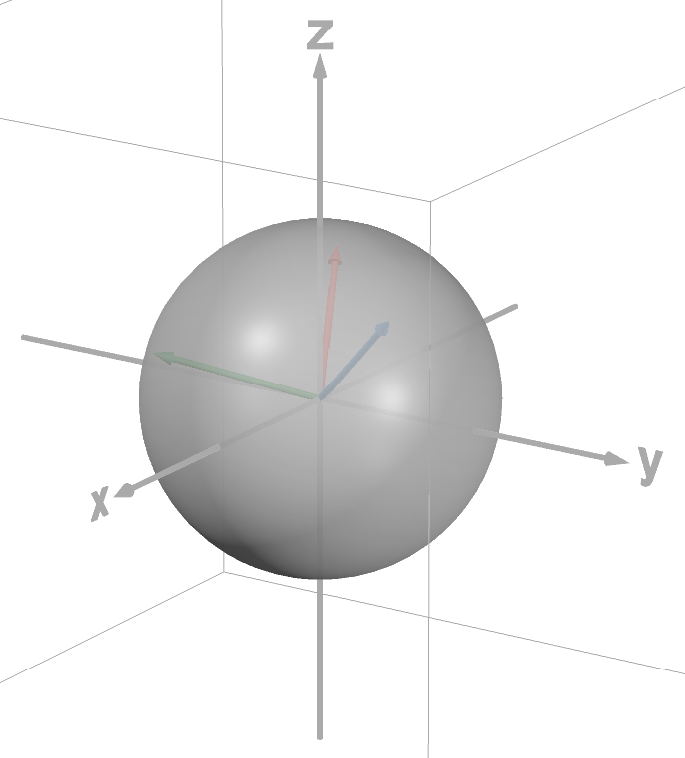
\includegraphics[width=60mm]{Images/S}  \qquad
	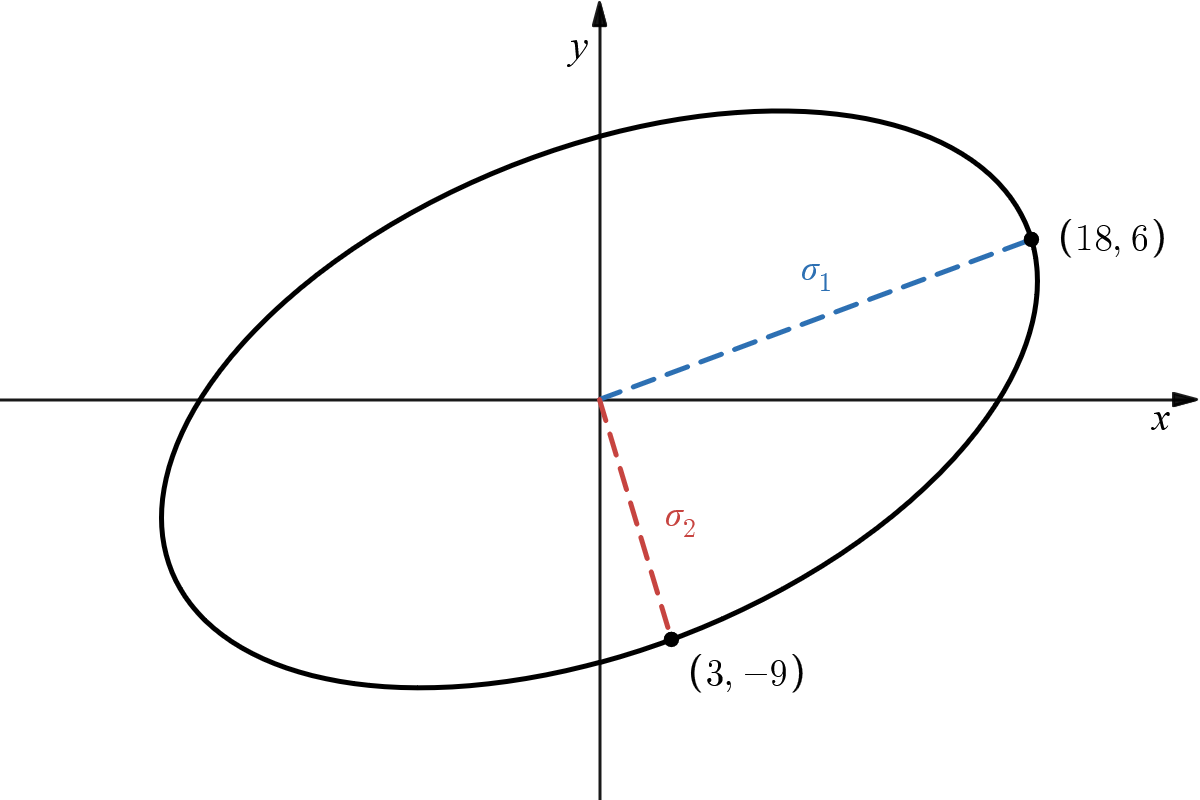
\includegraphics[width=90mm]{Images/AS}
\caption{Left: Right singular vectors of $A$ as seen as vectors landing on the unit sphere $S$ in $\R^3$ (see also \href{https://www.desmos.com/3d/rqqkklpdaj}{this} Desmos page). Red and blue vectors go to the red and blue axes in the picture to the right, green axis is sent to 0. 
Right: the image $AS$ of the unit sphere under $A$. The two principle directions of the ellipse are shown, the blue axis has $\sigma_1=6\sqrt{10}$ and points in direction $u_1$, red has length $\sigma_2=3\sqrt{10}$ and points in direction $u_2$.}
\label{fig:singval}
\end{figure}

 Suppose $A$ is the $3\times 2$ matrix \[ A=\m{4 & 11 & 14 \\ 8 & 7 & -2}\] from our previous example. Then $A$ represents a linear transformation $\R^3\to\R^2$. Let $S$ be the unit sphere in $\R^3$ (i.e., $x^2+y^2+z^2=1$) and \[AS =\{Av : v\in S\}\] be the image of the unit sphere under $A$ (as a region in $\R^2$). In this case, $AS$ is an ellipse: the major and minor radii are $6\sqrt{10}$ and $3\sqrt{10}$ respectively (the singular values of $A$), and occur along the axes in $\R^2$ given by the corresponding left singular values of $A$, the columns of the matrix $U$. The right singular values of $A$ denote the axes in the domain which get sent to each of these axes in $\R^2$: the first two columns of $V$ go to the major and minor axes of $AS$, respectively, and the third column (corresponding to singular value $\sigma_3=0$) gets ``crushed'' (note that a linear transformation $\R^3\to\R^2$ cannot be injective). This is all summarized in Figure \ref{fig:singval}.



In general, when finding the singular value decomposition of an $m\times n$ matrix $A$ you determine: 
\begin{itemize}
	\item The image of the unit ``sphere'' $S$ in $\R^n$ under the matrix $A$. This will always be an ``ellipsoid'' $AS$ of dimension $k=\rank{A}$ living in $\R^m$
	\item The principle axes of $AS$ along with the ``radii'' of the ellipse along these axes
	\item The axes in $\R^n$ which get sent to each principle axis of $AS$, along with all axes which get crushed by the transformation $A$
\end{itemize}
That's it. Since singular value decomposition can be applied to \textit{any} matrix $A$, this gives a canonical way to understand any given linear transformation. They takes spheres to ellipsoids, that's about it. See Appendix \ref{app-image} for an example of how singular value decomposition can be used in digital image processing. 


\subsection{Exercises} 

\begin{enumerate}[label=\arabic*.]
\item For each of the following symmetric matrices (i) compute an orthonormal basis of eigenvectors for the matrix, and (ii) determine the spectral decomposition of that matrix
\begin{enumerate}
	\item $\m{ 3 & 1 \\ 1 & 3}$
	\item $\m{1 & -6 & 4 \\ -6 & 2 & -2 \\ 4 & -2 & -3}$
	\item $\m{5 & 8 & -4 \\ 8 & 5 & -4 \\ -4&-4&-1}$
\end{enumerate}

\item Determine the singular value decomposition of the following matrices

\begin{enumerate}
	\item $\m{-1 & 1 \\ 6 & 2\\ 6 & 2}$
	\item $\m{1 & 1 \\ 0 & 1 \\ -1 & 1}$
	\item $\m{3 & 2 & 2 \\ 2 & 3 & -2}$
	\item *$\m{6 & -8 & -4 & 5 & -4 \\ 2 & 7 & -5 & -6 & 4 \\ 0 & -1 & -8 & 2 & 2 \\ -1 & -2 & 4 & 4 & -8}$
\end{enumerate}

\item Prove proposition \ref{prop:symrank}

\item Let $u\in \R^n$ be a unit vector and set $B=uu^T$. 
\begin{enumerate}
	\item Show that $Bx=\proj{u}{x}$ for any $x\in \R^n$.
	\item Show that $B$ is symmetric and $B^2=B$
	\item Show that $u$ is an eigenvector of $B$ and determine the corresponding eigenvalue

\end{enumerate}

\item Show that a matrix $A$ is symmetric if and only if $(Ax)\cdot y=x\cdot (Ay)$ for all vectors $x,y\in \R^n$\footnote{If a linear transformation $T$ on $\R^n$ satisfies $\langle Tx,y\rangle=\langle x,Ty\rangle$ (here, $\ip{\,}{}$ is some inner product on $\R^n$) for all $x,y\in \R^n$, then $T$ is called \textit{self-adjoint}. This problem shows that self-adjoint operators on $\R^n$ are represented by symmetric matrices, at least with the inner product of the dot product}.
\item Show that if $A$ is an $n\times n$ matrix, then the product of the singular values of $A$ is equal to $|\det A|$.

\item Show that if $P$ is orthogonal, then $PA$ and $A$ have the same set of singular values

\item Let $A$ have singular value decomposition $A=U\Sigma V^T$. Show that the columns of $V$ are eigenvectors of $A^TA$, and that the columns of $U$ are eigenvectors of $AA^T$. 




\item This problem concerns some computations with exterior products of vectors, in particular it will show in more detail why the spectral decomposition \eqref{eq-spec0} comes about.
\begin{enumerate}
\item Let $\{e_1,\cdots,e_n\}$ be the standard basis of $\R^n$ and define $E_{i,j}=e_ie_j^T$. Show that $\{ E_{i,j} : 1\leq i\leq n, 1\leq j\leq n\}$ is a basis for the vector space of $n\times n$ matrices. 
\item Let $A=\m{a_1 & \cdots & a_n}$ and $B=\m{b_1 & \cdots & b_n}$ be $n\times n$ matrices. Show that \begin{equation} AB^T=a_1b_1^T + \cdots + a_nb_n^T \end{equation}

(\textit{Hint}: Write $A=\m{a_1 & 0 & \cdots & a_n}+\m{0 & a_2 & \cdots & 0}+\cdots+\m{0 & 0 & \cdots & a_n}$ and then show for $i=1,\cdots,n$ that \[ \m{0 & \cdots & 0 & a_i & 0 & \cdots & 0} B^T=a_ib_i^T\]


\item Let $A$ be an $m\times n$ matrix with nonzero singular values $\sigma_1,\cdots,\sigma_r$ such that $A$ has singular value decomposition $A=U\Sigma V^T$ with $U=\m{u_1 & \cdots & u_m}, V=\m{v_1 & \cdots & v_n}$ the matrices of left- and right- singular values of $A$. Show that  
	\[A=\sigma_1 u_1v_1^T+\cdots \sigma_r u_r v_r^T\]
	as proposed in \eqref{eq-sing}.
\end{enumerate}
\end{enumerate}
Additional suggested exercises: \textit{Lay} sections 7.1, 7.4, 7.5



\newpage

 
\appendix



\section{Inverse matrix theorem} \label{ap-inv-mat-thm}

\begin{thm}[The invertible matrix theorem]
	Let $A$ be an $n\times n$ matrix. The following are equivalent
	\begin{enumerate}
		\item $A$ is invertible
		\item $A$ is equivalent by row operations to the identity matrix
		\item $A$ has $n$ leading 1s in its reduced echelon form
		\item The equation $Ax=\vec{0}$ has only the trivial solution
		\item The nullspace of $A$ is $\{\vec{0}\}$. 
		\item The columns of $A$ are linearly independent
		\item The linear transformation $x\mapsto Ax$ is one-to-one
		\item The equation $Ax=b$ has a solution for each $b\in\mathbf{R}^n$
		\item The columns of $A$ span $\mathbf{R}^n$
		\item The linear transformation $x\mapsto Ax$ is onto
		\item There is an $n\times n$ matrix $C$ such that $CA=I$
		\item There is an $n\times n$ matrix $D$ such that $AD=I$
		\item $A^T$ is invertible
		\item $\det{A}\neq 0$
		\item The columns of $A$ form a basis of $\mathbf{R}^n$
		\item The rows of $A$ form a basis of $\mathbf{R}^n$
		\item $\col{A}\cong \mathbf{R}^n$.
		\item $\rank{A}=n$
		\item $\dim \nul{A}=0$
		\item The nullity of $A$ is 0
		\item $0$ is not an eigenvalue of $A$
		\item $(\col{A})^{\perp}=\{\vec{0}\}$
		\item $(\nul{A})^{\perp}=\R^n$
		\item $\row{A}=\R^n$
		\item $A$ has $n$ nonzero singular values
	\end{enumerate}
\end{thm}


\section{Inverses and the adjugate matrix}\label{ap-adjugate}

\subsection{A general form of inverse matrices}
Let $A$ be an $n\times n$ matrix and assume that $\det{A}\neq 0$. Then we know that $A$ has an inverse. Recall that $A_{i,j}$ denotes the $i,j$ cofactor matrix of $A$---this is an $(n-1)\times (n-1)$ submatrix of $A$. The \textbf{cofactor matrix} of $A$ is the matrix $C_A$ given by \begin{equation} (C_A)_{i,j}= (-1)^{i+j} \det(A_{i,j})\end{equation}

For instance, $A$ is the $3\times 3$ matrix $A=\begin{pmatrix} a & b & c \\ d & e & f \\ g & h & i\end{pmatrix}$ then 
\[C_A=\begin{pmatrix} 
	\det \begin{pmatrix} e & f \\ h & i \end{pmatrix} & -\det \begin{pmatrix} d & f \\ g & i \end{pmatrix} & \det \begin{pmatrix} d & e \\ g & h \end{pmatrix} \\
	&&\\
	-\det \begin{pmatrix} b & c \\ h & i \end{pmatrix} & \det \begin{pmatrix} a & c \\ g & i \end{pmatrix} & -\det \begin{pmatrix} a & b \\ g & h \end{pmatrix}\\
	&&\\
	\det \begin{pmatrix} b & c \\ e & f \end{pmatrix} & -\det \begin{pmatrix} a & c \\ d & f \end{pmatrix} & \det \begin{pmatrix} a & b \\ d & e \end{pmatrix}
\end{pmatrix}\]
\begin{defn}Given an $n\times n$ matrix $A$, the \textbf{adjugate} of $A$, written $\adj{A}$, is the transpose of the cofactor matrix of $A$. That is, $\adj{A}=C_A^T$, or, in components \begin{equation} \adj{A}_{i,j}=(-1)^{i+j} \det{A_{j,i}}\end{equation}
\end{defn}
\begin{example}For the $2\times 2$ matrix $A=\begin{pmatrix} a & b \\ c & d\end{pmatrix}$ the adjugate of $A$ is given by: \[ \adj{A}=\begin{pmatrix} d & -b \\ -c & a\end{pmatrix}\]
You may recall that if $\det{A}\neq 0$, then $\dfrac{1}{ad-bc}\begin{pmatrix} d & -b \\ -c & a\end{pmatrix}$ gives a description of the inverse of $A$. This motivates the following theorem 
\end{example}

\begin{thm}\label{thm-adjugate-inv}
	Let $A$ be an $n\times n$ invertible matrix. Then $A^{-1}$ is given explicitly by \begin{equation} 
		A^{-1}=\dfrac{1}{\det A} \adj{A}
\end{equation}
\end{thm}


\begin{remark}
	While Theorem \ref{thm-adjugate-inv} does give an explicit method for calculating the inverse of $A$, it's often more efficient still to use row reduction to solve for $A^{-1}$ (in general, the adjugate computation takes twice the number of computations as row reduction). For small matrices, you may find it's easier to use the adjugate to calculate the inverse, however\footnote{Admittedly, I could never remember what the adjugate was and made my way through undergrad and grad school only ever  using row operations}
\end{remark}


\section{Application: Digital image processing}
\label{app-image}
	One nifty application of singular value decomposition is to digital image processing. Consider the following picture of my cat Leo sleeping on (one of) his favorite blankets.
	\begin{figure}[h]
	\centering
	 
\includegraphics[width=75mm]{Images/leo}
	\caption{Leo enjoying a nap}
	\end{figure}
	
	This image is made from a $719\times 592$ array of pixels, each determined by red, green, and blue values (usually integers between $0$ and $255$). These can turned into three $719\times 592$ matrices $R$, $G$, $B$ whose entries are the intensities of each of these colors. Suppose we look at the red matrix $R$. $R$ has $592$ singular values $\sigma_1,\cdots, \sigma_{592}$, some of which might be 0, which can be computed. If we arrange these in descending magnitude, we can compress the image by retaining the largest singular values while throwing away any that fall beneath some intensity threshold. This is a bit computationally taxing, the singular value decomposition needs to be applied three times (once to each matrix $R$, $G$ and $B$), but is in some sense the ``most optimal'' image compression you could hope for\footnote{JPEG compression works similarly, but the ``basis'' matrices are set at the beginning, rather than ``dictated'' by the matrix you're trying to compress. Still neat.}.
	
	In figure \ref{fig:leo} you can find several different compressed photos of leo, along with the number of singular values used and the compression ratio. In fact, the singular values ``importance'' generally follows an exponential decay, by using 50 singular values most of the information is retained and a pretty high compression ratio is achieved. 
	
	\begin{figure}[h]
	\centering
	
	
\includegraphics[width=75mm]{Images/leo3} \quad 
\includegraphics[width=75mm]{Images/leo10} 
	
	\vspace{5mm}
	
	
\includegraphics[width=75mm]{Images/leo50} \quad 
\includegraphics[width=75mm]{Images/leo20} 
	
	\caption{ Starting top left, moving clockwise: 3 singular values used, compression ratio 81.11; 10 singular values, compression ratio 32.44; 20 singular values, compression ratio 16.22; 50 singular values, compression ratio 6.49. Credit to \href{https://timbaumann.info/svd-image-compression-demo/}{Tim Baumann} for the tools to make these photos.}
	
	\label{fig:leo}
	\end{figure}
\end{document}
\section{Notation}
\begin{itemize}
	\item $\mathbf{R}$ the set of real numbers
	\item $\mathbf{0}$ the trivial vector space $\{\vec{0}\}$. 

\end{itemize}
